



\documentclass[12pt,a4paper]{book}



			% Packages Files
%----------------------------------%

	% Page Setttings
\usepackage[top = 1in, bottom = 1in, left = 1in, right = 1in]{geometry}

\parindent=0cm % to prevent the spacing in new paragraph or new line

\usepackage{fancyhdr}
\setlength{\headheight}{14.5pt} % needded for header and footer 

%-----------------------------------------------------------------%

\usepackage{amsmath} % needed for referencing thequation
\usepackage{amsfonts} % for maths symbols
\usepackage{graphicx}
\usepackage[export]{adjustbox}
\usepackage{nomencl} % must be loaded before caption (KOMA tocbasic conflict)
\usepackage{caption}
\usepackage{refstyle} % to reference a captioned figure


% To make hyperlinks

\usepackage[
	colorlinks=true
	,breaklinks
	]{hyperref} % needed for creating hyperlinks in the document, the option colorlinks=true gets rid of the awful boxes, breaklinks breaks lonkg links (list of figures),
	
\usepackage{xcolor}
\definecolor{c1}{rgb}{0,0,1} % blue
\definecolor{c2}{rgb}{0,0.3,0.9} % light blue
\definecolor{c3}{rgb}{0.3,0,0.9} % red blue
\hypersetup{
    linkcolor={c1}, % internal links
    citecolor={c2}, % citations
    urlcolor={c3} % external links/urls
}

	% For Code Writing
	
\usepackage{listings}

\usepackage{color}

\definecolor{mygreen}{rgb}{0 0.6 0}

\lstset{
% Set automatic Line breaking, in case we have long lines don't
% fit inside the frame or the page.
breaklines = true,
commentstyle = \color{mygreen},
breakatwhitespace = true,% don't show white space character
%numbers = left, % put line number in the code
title = \lstname
}

% ------------- For Writing Equations inisde a table and centering them ------------

\usepackage{array}

% Vertical Alignment inside the cells of the table
\newcolumntype{M}[1]{>{\centering\arraybackslash}m{#1}}

% Horizontal Alignment inside the cells of the table
\newcolumntype{P}[1]{>{\centering\arraybackslash}p{#1}}


% needed for todos liste
\usepackage{todonotes} 



% %---------- needed for long tables over pages-------
\usepackage{longtable} 

\usepackage[acronym]{glossaries}




% Macros File

% Macros Example
\def\labelaxes{Remember to include some suitable labeling for the axes and the units used in measurements.}

% 2nd way for defnining macros: the new command
% 1st parameter: name of the new command
% 2nd paramter: how many inputs this command needs, in this case only 1
% 3rd parameter: what this new command named \tbi do

\newcommand{\tbi}[1]{\textbf{\textit{#1}}}

% Command for Picture without a label

\newcommand{\pic}[3]{\begin{figure}[h]
\centering
\includegraphics[width = 0.7\textwidth, frame]{#1}
\caption{#2}
\end{figure}}








\DeclareMathOperator*{\argmax}{argmax} % thin space, limits underneath in displays

\DeclareMathOperator*{\argmin}{argmin}

\title{Signal Processing Simulations}
\author{Ranim Tom}


%******** Abbreviations **********

% to change the name of Nomenclature to list of abbreviation
\renewcommand{\nomname}{List of Abbreviations}

% for list of abbreviations and acronyms
\makenomenclature

%******** End Abbreviations **********

% to make the list of abbreviations and acronyms appear 
% in first pages of the report
\printnomenclature


\makeglossaries
\newacronym{dft}{DFT}{Discrete Fourier Transform}

\begin{document}

% downloaded template
%\input{content/title_page_1} 

\maketitle

\tableofcontents







% to make the todo list appear as a table of content
\listoftodos

% list of notation I use in DSP







\chapter*{List of Notations}

\begin{longtable}{c|c}
Notation & Description \\ \hline
$x(t)$ & Continuous time signal \\ \\
$x_s(t)$ & Sampled Signal \\ \\
$x[n]$ & Discrete time signal \\ \\
$x^{(i)}(t)$ & $i^{th}$ order derivative of $x(t)$ \\ \\
$F_s$ & Sampling Rate \\ \\
$T_s$ & Sampling Period \\ \\
$F$ & Analog Frequency in Hz \\ \\
$\Omega$ & Analog Angular Frequency in rad/s \\
& such that $\Omega \, = \, 2 \, \pi \, F $ \\ \\
$\omega$ & Normalized angular frequency in rad/sample \\
& such that $ -\pi \, \leq \, \omega \, \leq \, \pi$ \\ \\
$F_{s_{\text{ch}}} \, , \, T_{s_{\text{ch}}}$ & Sampling rate and sampling period per channel respectively \\ \\
$\tau$ & delay  \\ \\
$\alpha$ & scaling factor (can be $<$ or $>$ 1) \\ \\
$\star$ & convolution operation \\ \\
$K$ & Total Number of channels \\ \\
$\dagger$ & Pseudo Inverse Operation \\ \\
$\displaystyle\left\lfloor \frac{}{} \right\rfloor$ and $\displaystyle\left\lceil \frac{}{} \right\rceil$ & rounding down and up to the nearest integer respectively


\end{longtable}






\pagestyle{fancy}
\fancyhf{} % Clear header and footer
\rhead{\rightmark}
\lhead{Chapter \thechapter}
\rfoot{Page \thepage}




\chapter{Sampling and Reconstruction}
\label{Chap:Sampling_Reconstruction}

\todo{Sampling and Reconstruction}

\begin{itemize}

\item \textit{To work on some example with sinc interpolation}

\item \textit{Include simulation examples from papoulis for example}

\end{itemize}


\chapter{Fourier Transform}

\section{Introduction}

This chapter include simulation about spectral analysis using tools such as Discrete Fourier Transfrom (DFT) \nomenclature{DFT}{Discrete Fourier Transfrom} and Fast Fourier Transform (FFT) \nomenclature{FFT}{Fast Fourier Transform}.

\section{Reminder}

\subsection{Fourier Transform Relation}

\underline{Notation:} taken from chapter 4 in \cite{DSP_DimitrisManolakis}

\begin{table}[!h]
	\centering
\begin{tabular}{|c|c|c|} \hline

Time: Continuous or Discrete & Analysis (Frequency Domain) & Synthesis (Time Domain) \\ \hline
CTFS & $c_k \, = \, \displaystyle\frac{1}{T_0} \displaystyle\int_{T_0} x(t) \, e^{-j  \, k \, 2 \pi f_0 t} dt$ 	& $x(t) \, = \, \displaystyle\sum_{k \, = \, - \infty}^{+ \infty} c_k \, e^{j \, k \, 2 \pi F_0 \, t}$   \\ \hline
CTFT & $X(F) \, = \, \displaystyle\int_{-\infty}^\infty x(t) \, e^{-j 2\pi F t} dt $	& $x(t) \, = \, \displaystyle\int_{-\infty}^\infty X(F) \, e^{j 2\pi F t} dF $ \\ \hline
DTFS    & $c_k \, = \, \displaystyle\frac{1}{N} \displaystyle\sum_{n \, = \, 0}^{N \, - \, 1} x[n] \, e^{-j  \, \frac{2 \pi}{N} \, k \,n} $ & $x[n] \, = \, \displaystyle\sum_{k \, = \, 0}^{N \, - \, 1} c_k \, e^{j  \, \frac{2 \pi}{N} \, k \,n}$ \\ \hline
DTFT    & $X(\omega) \, = \, \displaystyle\frac{1}{N} \displaystyle\sum_{n \, = \, - \infty}^{\infty} x[n] \, e^{-j  \, \omega \,n} $ & $x[n] \, = \, \displaystyle\int_{2 \pi} X(\omega) \, e^{j  \, \omega \,n} d \omega$ \\ \hline
\end{tabular}
\caption{Fourier Formula}
\label{Tb:Fourier_Processing:Fourier_Relation}
\end{table} 


\newpage
\subsection{Frequency Variables}

\begin{itemize}

\item Relation between \textit{continous frequency} $F$ [Hz] and \textit{continous angluar frequency} $\Omega$ [rad/s]:

\begin{equation}
\Omega \, = \, 2 \pi \, F
\label{eq:Omega_Fs}
\end{equation}

\item Relation between \textit{normalized angular frequency} $\omega$ [rad/cycle] and \textit{continuous angular frequency} $\Omega$ [rad/s] \cite{DSP_DimitrisManolakis}
    
\begin{equation}
    \omega  = \displaystyle\frac{\Omega}{F} 
\end{equation}

\item Moving between Hz $\leftrightarrow$ [rad/cycle]

\begin{table}[!h]
	\centering
\begin{tabular}{|c|c|} \hline
radian/cycle $\rightarrow$  Hz & Hz $\rightarrow$ radian/cycle \\ \hline 
 $ F \, [\text{Hz}] \, = \, \omega [\text{radian/cycle}] \, \times \, \left( \, \displaystyle\frac{F_s}{2 \pi} \, \, \right)$ & $\omega \, [\text{radian/cycle}] \, = \, F [\text{Hz}] \, \times \, \left( \, \displaystyle\frac{2 \pi}{F_s} \, \right)$ \\ \hline
\end{tabular}
\caption{Fourier Formula}
\label{Tb:Fourier_Processing:frequency_variables}
\end{table} 

\item Diagram illustration of \autoref{Tb:Fourier_Processing:frequency_variables}\cite{DSP_DimitrisManolakis}



\begin{figure}[h]
\centering
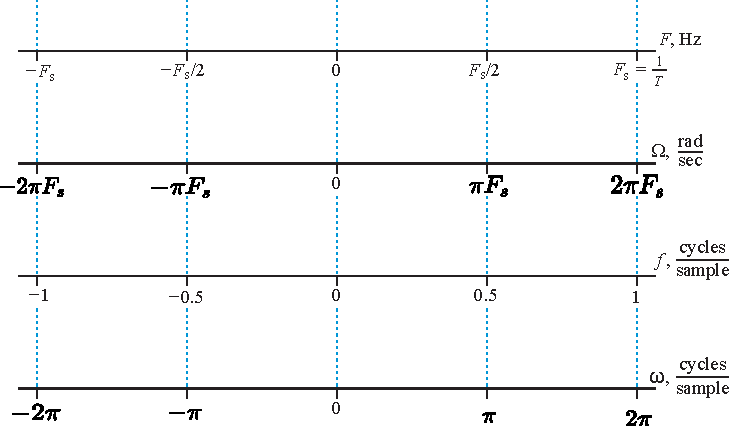
\includegraphics[scale = 1.2]{Figures/Fourier_Summary/frequency_variables}
\label{fig:Fourier_Summary:frequency_variables}
\caption{Frequency Variables illustration of \autoref{Tb:Fourier_Processing:frequency_variables}\cite{DSP_DimitrisManolakis}}
\end{figure}

\end{itemize}


\newpage
\subsection{DTFT-CTFT Relation}


See \cite{signal_processing_Lathi}.

\begin{equation}
\begin{array}{lll}
X_{\delta}(F) \, &=& \, \displaystyle\frac{1}{T_s} \displaystyle\sum\limits_{k \, = \, -\infty}^{+ \infty} X_c \left(\, F \, - \, k \,F_s  \,\right) \\ \\
                &=& \, X(\omega)
\end{array}
\label{Eq:DTFT-CTFT-Relation}
\end{equation}

\begin{itemize}
    \item $X(\omega)$ is an DTFT of $x[n] \leftrightarrow$ DTFT of a discrete signal
    
    \item $X_c(F)$: CTFT of the $x(t) \leftrightarrow$ CTFT of a analog continous signal
    
    \item $X_{\delta}(F)$: CTFT of $x(n \, T_s) \leftrightarrow$ CTFT of a sampled signal 
    
\end{itemize}

\autoref{Eq:DTFT-CTFT-Relation} states that DTFT and CTFT of a sampled signal are the same, and if we want to retrieve the CTFT of $x(t)$, we need to multiply by $T_s$

\todo{DTFT-CTFT Relation}: \textit{to insert a figure for \autoref{Eq:DTFT-CTFT-Relation}}.


\subsection{Fourier Transform Table}

\begin{table}[!h]
	\centering
\begin{tabular}{|c|c|} \hline
$x(t)$  & $X(F)$ \\ \hline 
$\Pi\displaystyle \left( \, \frac{t}{\tau} \,\right)$ & $\text{sinc} (\pi \, F \, \tau)$ \\ \hline
$2\, B \, \text{sinc}(2 \pi \, B \, t)$ & $\Pi\displaystyle \left( \, \frac{F}{2 \, B} \,\right) $\\ \hline
$\Delta\displaystyle \left( \, \frac{t}{\tau} \,\right)$ & $ \displaystyle\frac{\tau}{2} \, \text{sinc}^2 \left( \displaystyle\frac{\pi \, F \, \tau}{2}   \right)$ \\ \hline
$ B \, \text{sinc}(\pi \, B \, t)$ & $\Delta\displaystyle \left( \, \frac{F}{2 \, B} \,\right) $\\ \hline
 $\displaystyle\sum_{n \, = \, - \infty}^\infty \delta(t \, - \, n \, T_0)$ & $ f_0 \, \displaystyle\sum_{n \, = \, - \infty}^\infty \delta(F \, - \, n \, f_0)$ \\ \hline
\end{tabular}
\caption{CTFT Transform Pair}
\label{Tb:Fourier_Processing:CTFT_Table}
\end{table} 

\newpage
\section{Analog Signal}

\underline{Source:} see example 5.8 in \cite{signal_processing_Lathi},\\

The continuous time domain signal to be taken is a decaying exponential:

\begin{equation}
x(t) \, = \, \text{exp}(-0.5 \, t) \, u(t) \leftrightarrow \, X(\Omega) \, = \, \displaystyle\frac{1}{j \, \Omega \, + \, 0.5}
\label{eq:inf_time_freq}
\end{equation}

Signal of \autoref{eq:inf_time_freq} is infinite both in time and frequency domain.

$\mathrm{1}^\mathrm{st}$ step is to do an approximation in frequency domain, that is choosing the maximum frequency $B$. Once we have $B$, we can apply Nyquiste theorem to have an appropriate $F_s$ and hence a $T_s$, so we can truncate in time and obtain suitable number of samples.


\subsection{Truncation in frequency domain}

\begin{itemize}
    
\item Spectrum is infinite in frequency domain:    
    
Infinite in frequency domain means no maximum frequency to be taken to apply Nyquist sampling theorem $\rightarrow$ need to \tbi{truncate in frequency so we can choose a sampling frequency} $F_s$.\\

\item As a criteria to truncation: what is the value of $\Omega$ at which the frequency content is bellow 2 \% ? 

In other words, this $\Omega$ captures 98 \% of the frequency content of the signal.

\item \underline{Computations:} 

\begin{itemize}

\item $ \displaystyle\left\lvert X(\Omega) \displaystyle\right\rvert \, = \, \displaystyle\frac{1}{\sqrt{ \Omega^2\, + \, 0.5^2} } \, = \, 2 \, \times \, 0.01 \, = \, 0.02 $ 

\item Solving for $\Omega$ we get: $\Omega \, = \, 50 \text{ rad/s}$

\item Using \autoref{eq:Omega_Fs}: $B \, = \, \displaystyle\frac{\Omega}{2 \, \pi} \, = \, \displaystyle\frac{50}{2 \, \pi} \, = \displaystyle\frac{25}{\pi}$ Hz

\end{itemize}

\item The maximum frequency is $\displaystyle\frac{25}{\pi}$ Hz.

Applying Nyquiste states that $F_{s_{\text{min}}} \, = \, 2 \, B \, = \, 2 \, \times \, \displaystyle\frac{25}{\pi} \, = \, \displaystyle\frac{50}{\pi}$ Hz

\item Having $F_{s_{\text{min}}} \, = \, \displaystyle\frac{50}{\pi}$ gives a minimum sampling period $T_{s_{\text{min}}} \, = \, \displaystyle\frac{\pi}{50} $ s

\end{itemize}

So as summary, from frequncy truncation we get:

\begin{itemize}

\item $B \, = \, \displaystyle\frac{25}{\pi} \, \approx \, 8$ Hz

	\begin{itemize}
	\item This $B$ captures 98 \% of the frequency content of the signal
	\end{itemize}

\item $F_{s_{\text{min}}} \, = \, \displaystyle\frac{50}{\pi}$ Hz

\end{itemize}
  

\subsection{Truncation in time domain}

\begin{itemize}
    
\item Waveform in infinite in time domain:

After we solve for $T_s \, = \, \displaystyle\frac{\pi}{50}$ s, there is another question to be asked: for \tbi{how long do we need to sample} ? $\leftrightarrow$ This signal is going forever, we can't just keep sampling forever\\


So we need to solve for \tbi{sampling duration} $T_0 \, \leftrightarrow$  signal duration

\item \underline{Criteria to solve the problem:} We know that the signal is a decaying exponential, we can see for some value of $T_0$ where the  \tbi{amplitude value of the signal} $x(t)$  \tbi{is very low}, and by this we are \tbi{not throwing some high value amplitude (information)}.\\

\item Computing: 
	
	\begin{itemize}
	\item We try for example for $T_0 \, = \, 16$ s, we get $x(16) \, = \, e^{-0.5 \, (16)} = \, e^{-8} \, = \, 3.3 \, e^{-4}$, very small number
	
	\item If we choose $T_0 \, = \, 16$, the number of sample we get in this period using a sampling rate $T_s \, = \, \displaystyle\frac{\pi}{50}$ is: $N_0 \, = \, \displaystyle\frac{T_0}{T_s} \, = \, 254.65$
	
	
	\item However, the number of samples we need to grab need to be integer, so let's say we need to grab 256 samples
	
	\item We resolve again for $T_s$ using $N_0 \, = \, 256$ samples, and we get $T_s \, = \, \displaystyle\frac{1}{16}$ seconds 
\end{itemize}

\end{itemize}

The rest is done via programming part.\\

\subsection{Results}

\begin{figure}[h]
\centering
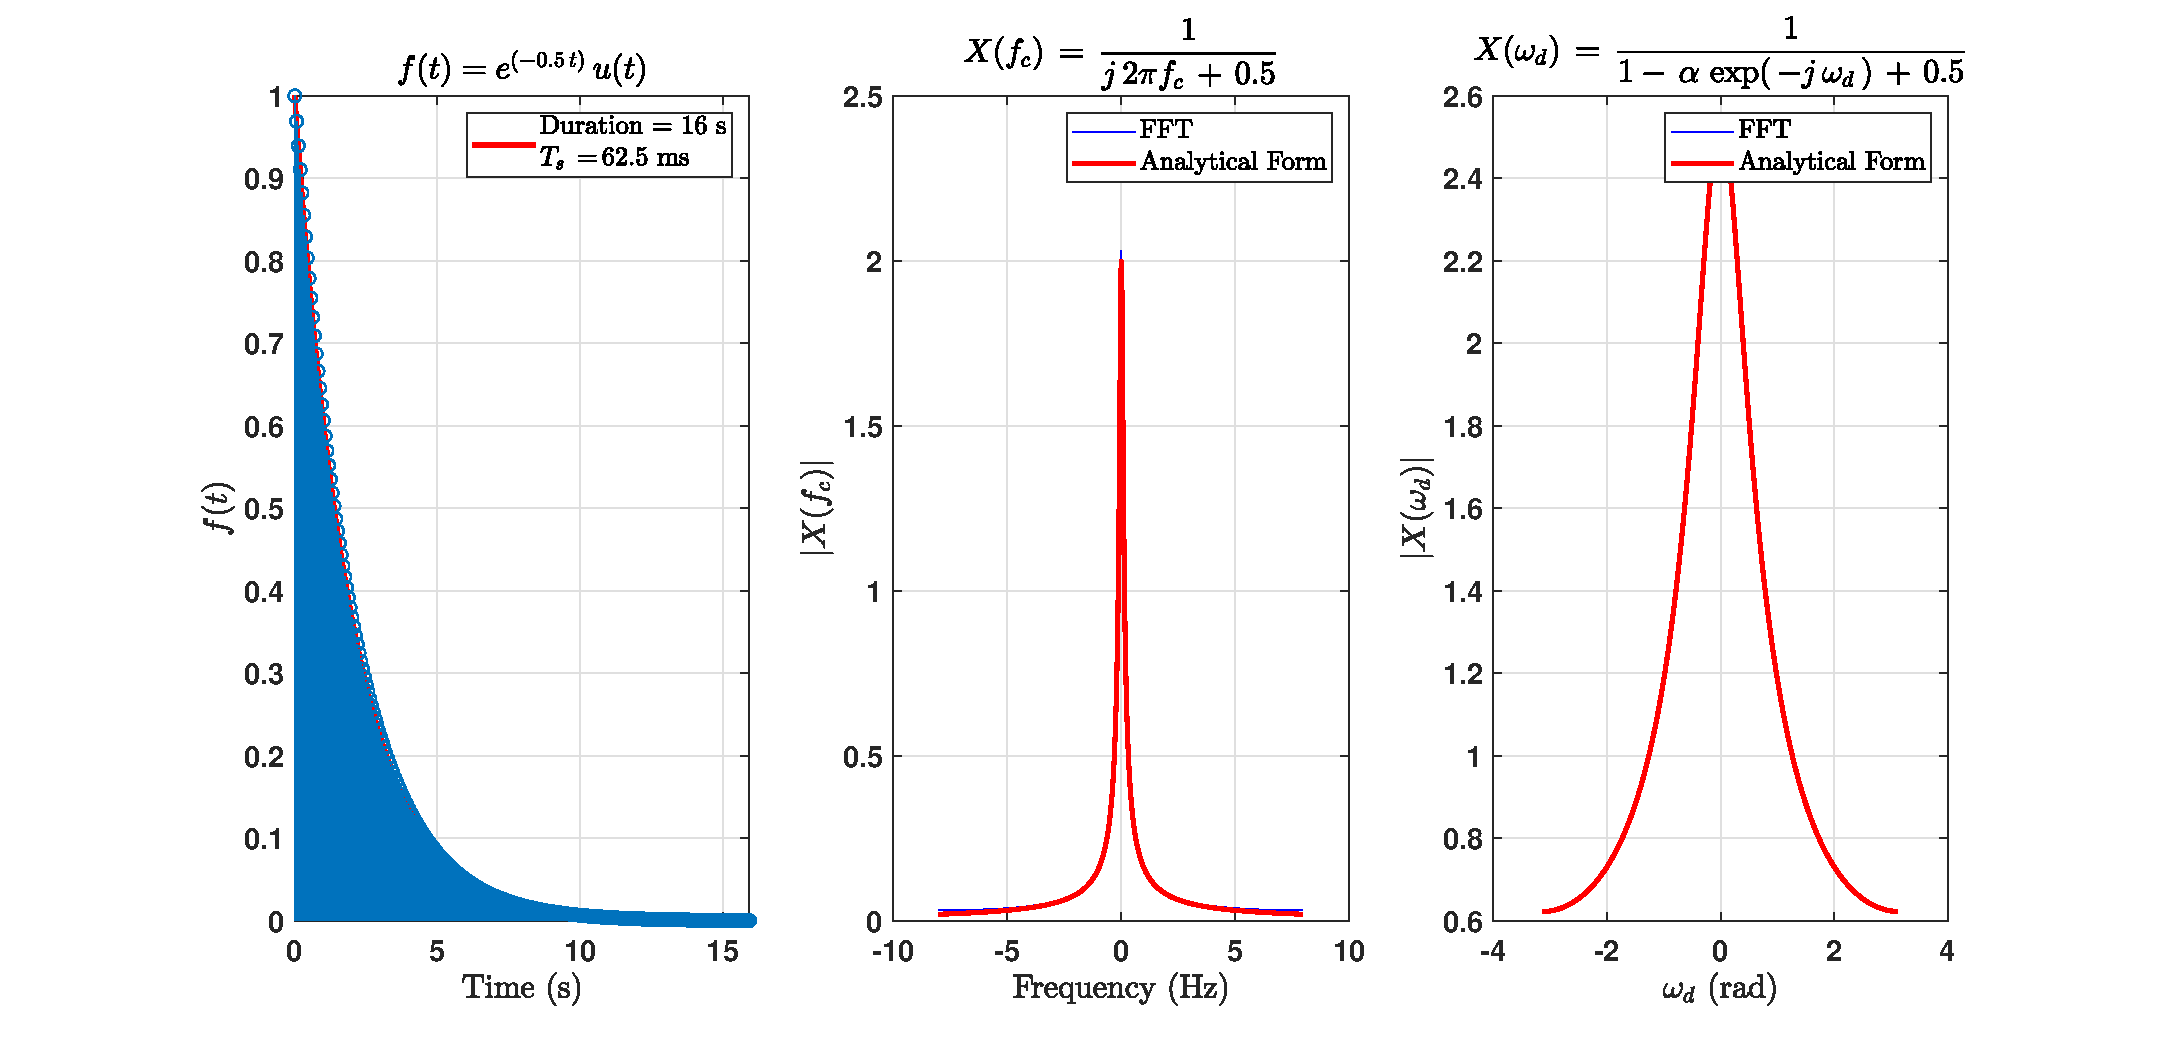
\includegraphics[scale = 0.5]{Figures/Sim_Fourier_Transform/CTFT_DTFT_using_fft_fs_16.eps}
\label{fig:Sim_Fourier_Transform:CTFT_DTFT_using_fft_fs_16}
\caption{Base line: Signal Duration is 16 s and $F_s \, = \,$ 16 Hz}
\end{figure}



\newpage
\subsection{Summary}

As a \tbi{summary} we have:

\begin{itemize}

\item $\mathrm{1}^\mathrm{st}$ question we ask since the signal $x(t)$ isn't band limited $\leftrightarrow$ keep going forever in frequency domain: \tbi{how do we choose the sampling rate (sampling period)} $F_s \, (T_s)$

	\begin{itemize}
	\item what is a suitable criteria to choose some maximum frequency to represent the bandwidth $B$ of the signal ?
	
	\item Once we choose $B$, we apply Nyquiste to have a minimum sampling frequency $F_{s_{\text{min}}}$
	\end{itemize}
	
\item $\mathrm{2}^\mathrm{nd}$ question: for \tbi{how long we keep sampling $\leftrightarrow$ (signal truncation)} ?

	\begin{itemize}
	\item choose some value of $T_0$ in which values (content) of the signal is preseverd
	
	\end{itemize}

\item Always recall that:
	
\begin{equation}
\overbrace{N}^{\text{nb of samples}} \, = \, \displaystyle\frac{\overbrace{T_0}^{\text{Signal duration}}}{\underbrace{T_s}_{\text{Sampling Period}}} \, \in \,\mathbb{N}
\end{equation}
	

\end{itemize}


\newpage
\section{Working with fft}

Now we turn attention to the usage of \verb|fft| command to compute the spectrum.\\

In \autoref{fig:Sim_Fourier_Transform:sinc2_B_10Hz_Fs_30Hz}, we have the result of $x(t) \, = \, B \, \text{sinc}(\pi \, B \, t) \leftrightarrow \, \Delta\displaystyle \left( \, \frac{F}{2 \, B} \,\right) $

\begin{figure}[h]
\centering
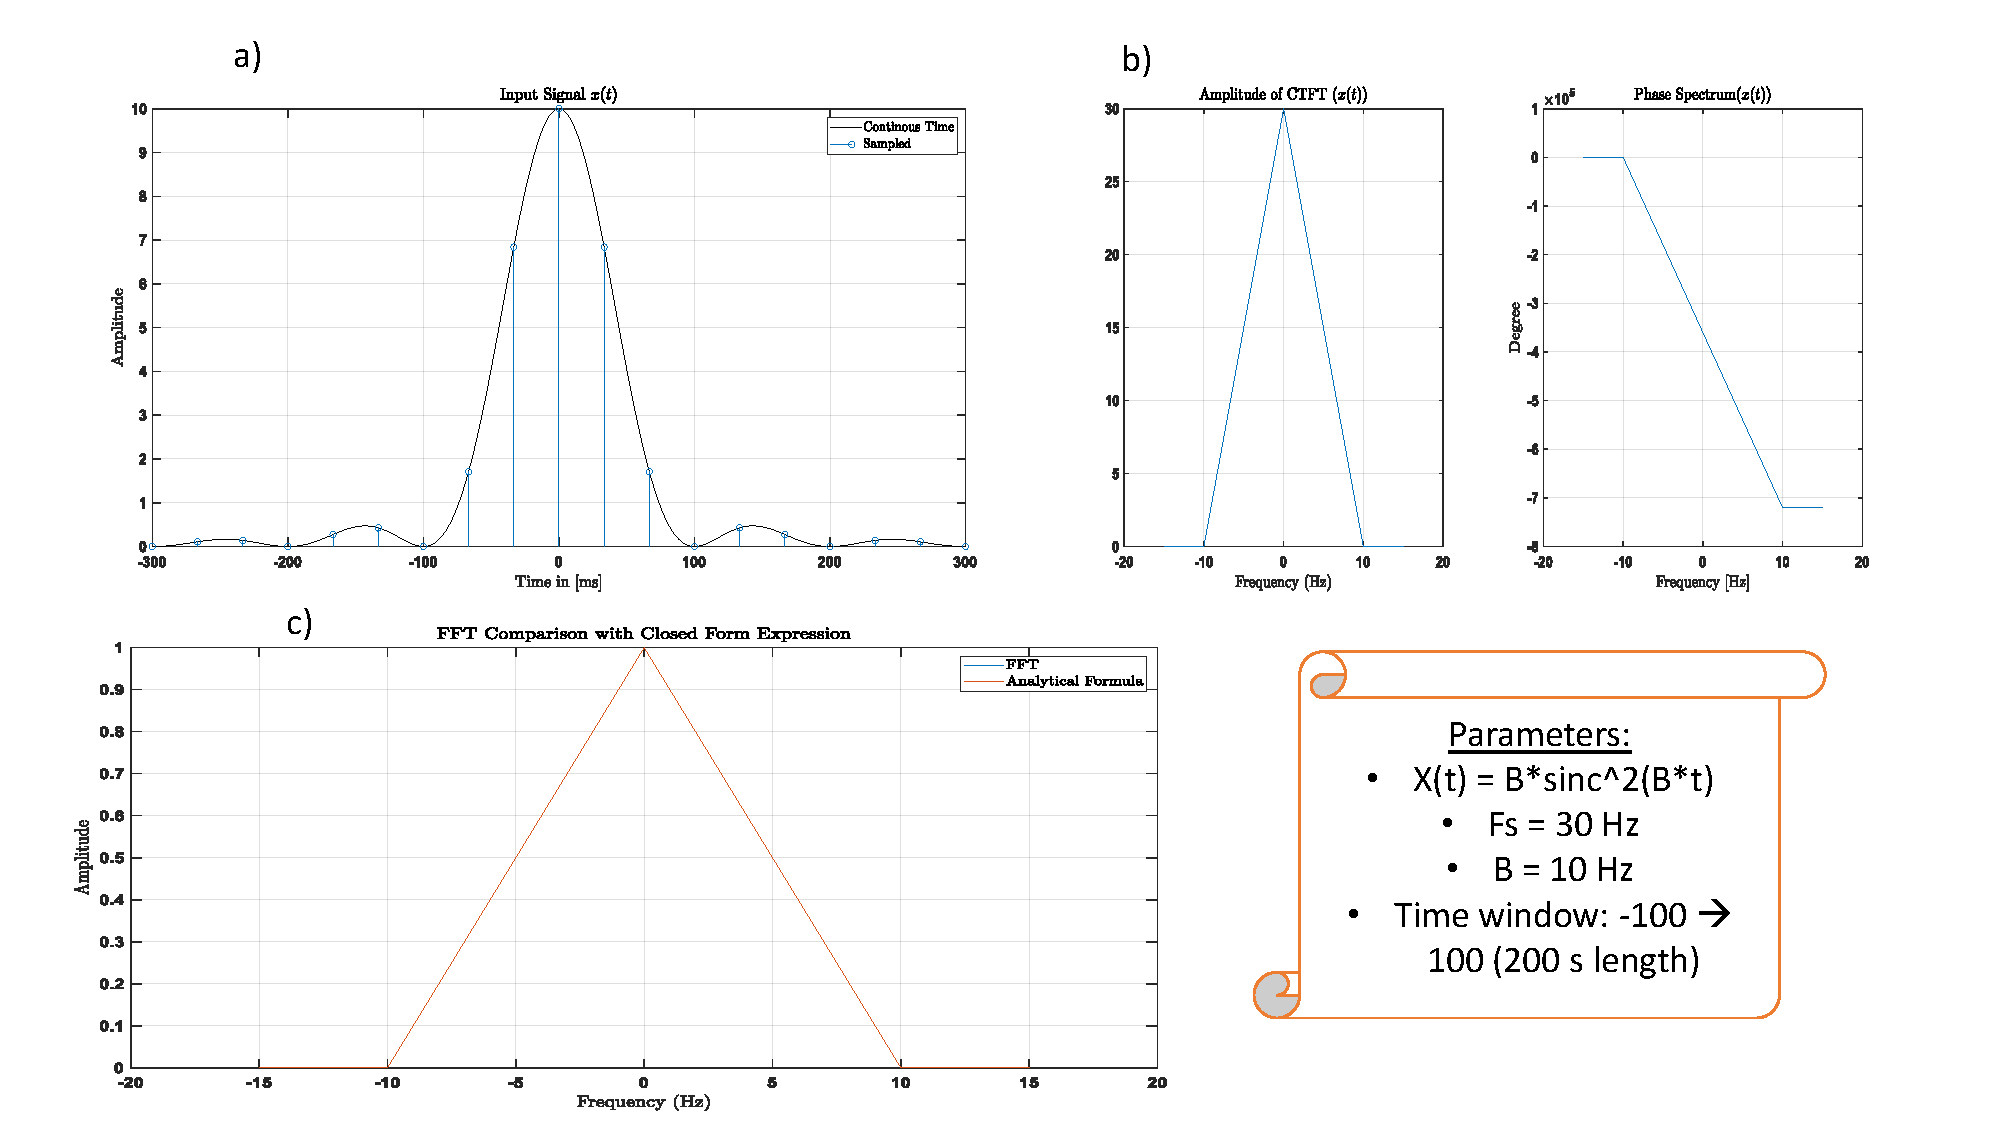
\includegraphics[scale = 0.5]{Figures/Sim_Fourier_Transform/sinc2_B_10Hz_Fs_30Hz}
\caption{Working with sinc square}
\label{fig:Sim_Fourier_Transform:sinc2_B_10Hz_Fs_30Hz}
\end{figure}

\begin{itemize}
    \item In order to obtain the unity amplitude in $\Delta\displaystyle \left( \, \frac{F}{2 \, B} \,\right)$, we need to divide by $F_s$ according to \autoref{Eq:DTFT-CTFT-Relation}.
\end{itemize}

\newpage
\subsection{Rect and Sinc Simulation}

Here are the result of some simulation for sinc and rect pulses presented in \autoref{fig:Sim_Fourier_Transform:res_sinc_rect_Fourier}


\begin{figure}[h]
\centering
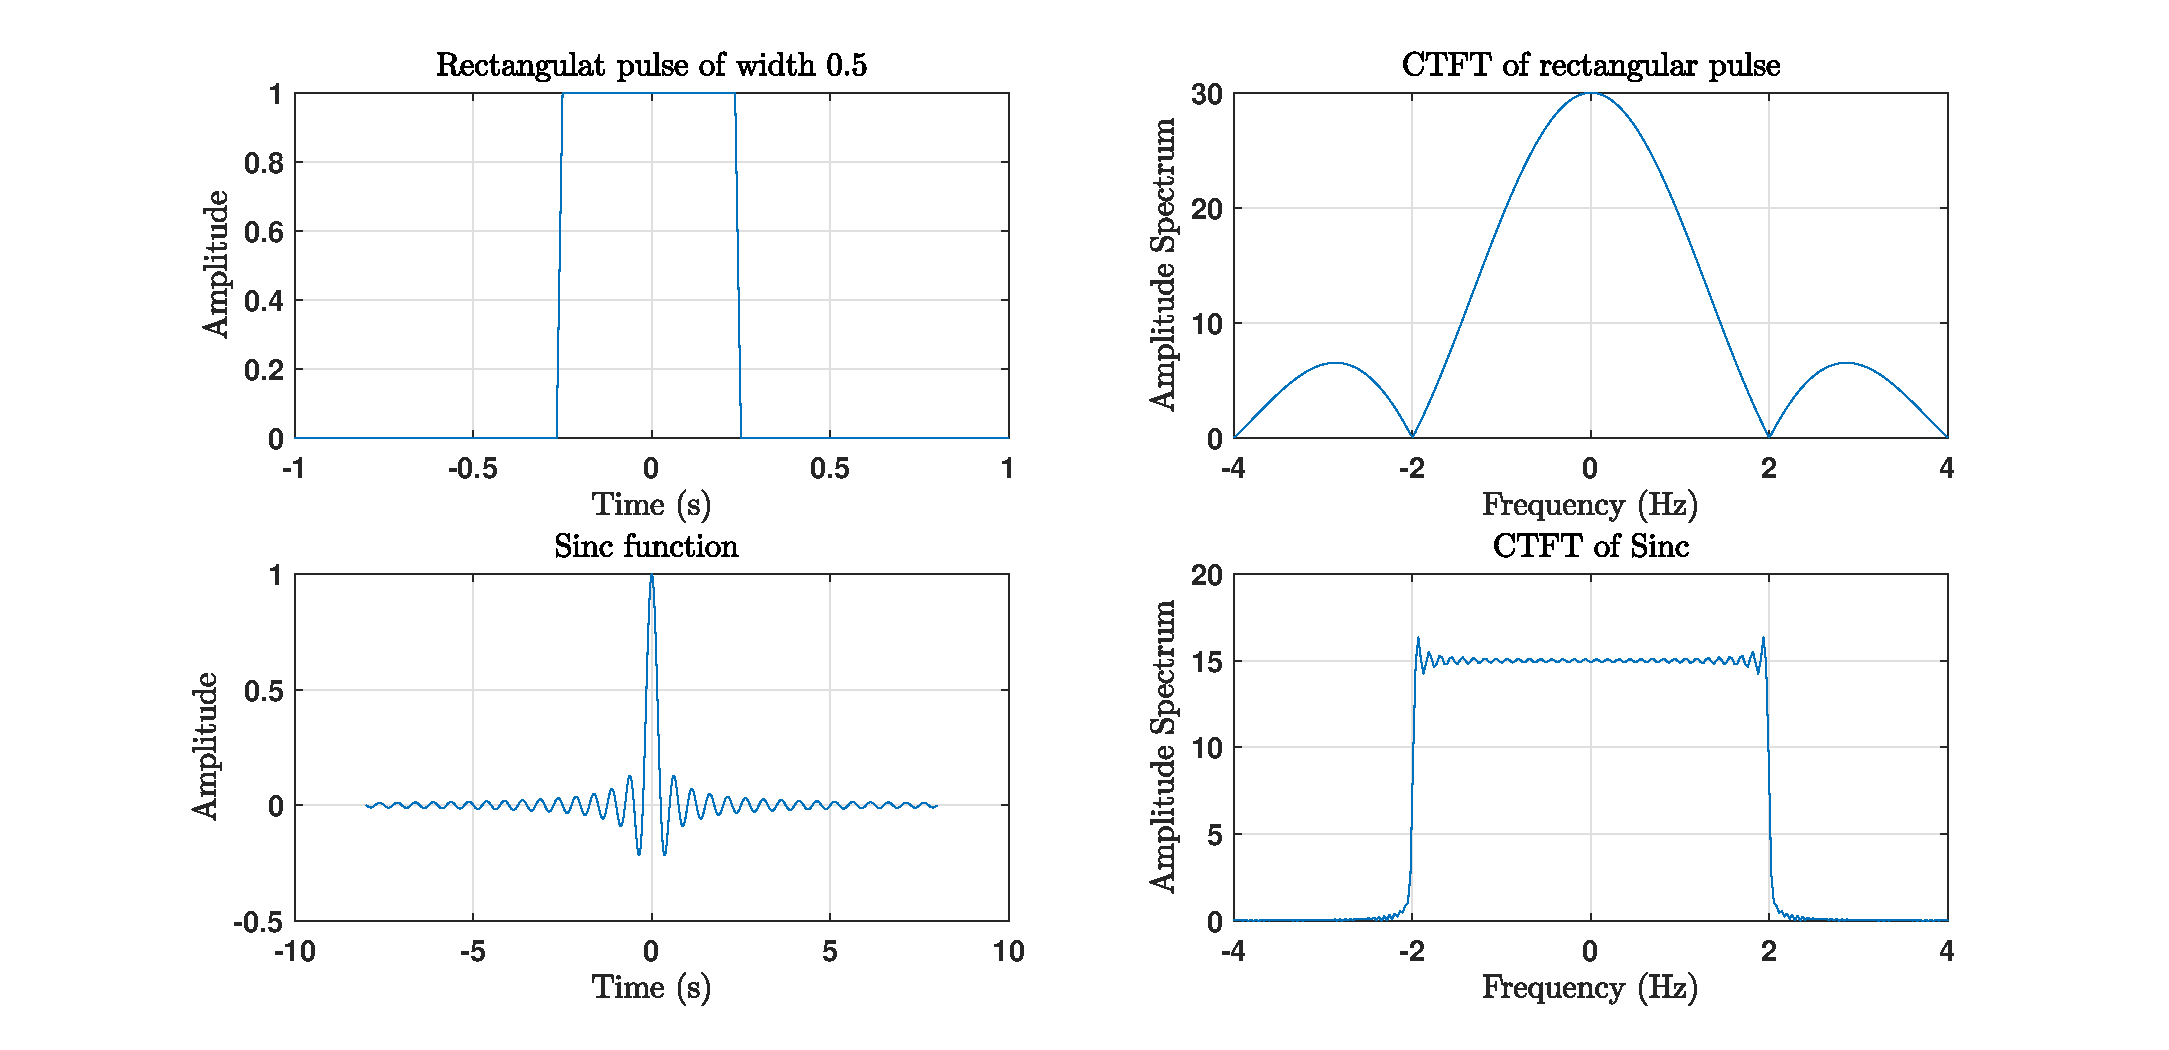
\includegraphics[scale = 0.5]{Figures/Sim_Fourier_Transform/res_sinc_rect_Fourier}
\caption{Plot of  $\text{rect} \left(\, \displaystyle\frac{t}{T} \, \right) \text{ and } \text{sinc}\left(\,  \displaystyle\frac{t}{T}  \, \right)$}
\label{fig:Sim_Fourier_Transform:res_sinc_rect_Fourier}
\end{figure}

\begin{itemize}
    \item $T$ is the pulse width for the sinc and rect
    
    \begin{itemize}
        \item for rect: the pulse width is divided in halfs before and after $t \, = \, 0$
        
        \item for sinc case: pulse wdith start from $t \, = \, 0$
        
    \end{itemize}
    
    \item Bandwidth:
    
    \begin{itemize}
        \item for rect: we have a null-to-null bandwdith equal ot $\displaystyle\frac{1}{T} \, = \, \displaystyle\frac{1}{0.5} \,  = \, 2$ Hz
        
        \item Same as for sinc: however the sinc is bandlimited unlike the rect: so after 2 Hz, we have 0 values for the amplitude spectrum
        
    \end{itemize}
    
\end{itemize}



\newpage

\section{IFFT}

\verb|ifft| command is used to take us back to the time domain given some discrete samples.\\

\underline{Note:} if the input of the \verb|ifft|,that is the complex vector (CTFT or DTFT) if shifted via \verb|fftshift| command, we need to undo it via \verb|ifftshift|.\\


\underline{Results:}

\begin{figure}[h]
\centering
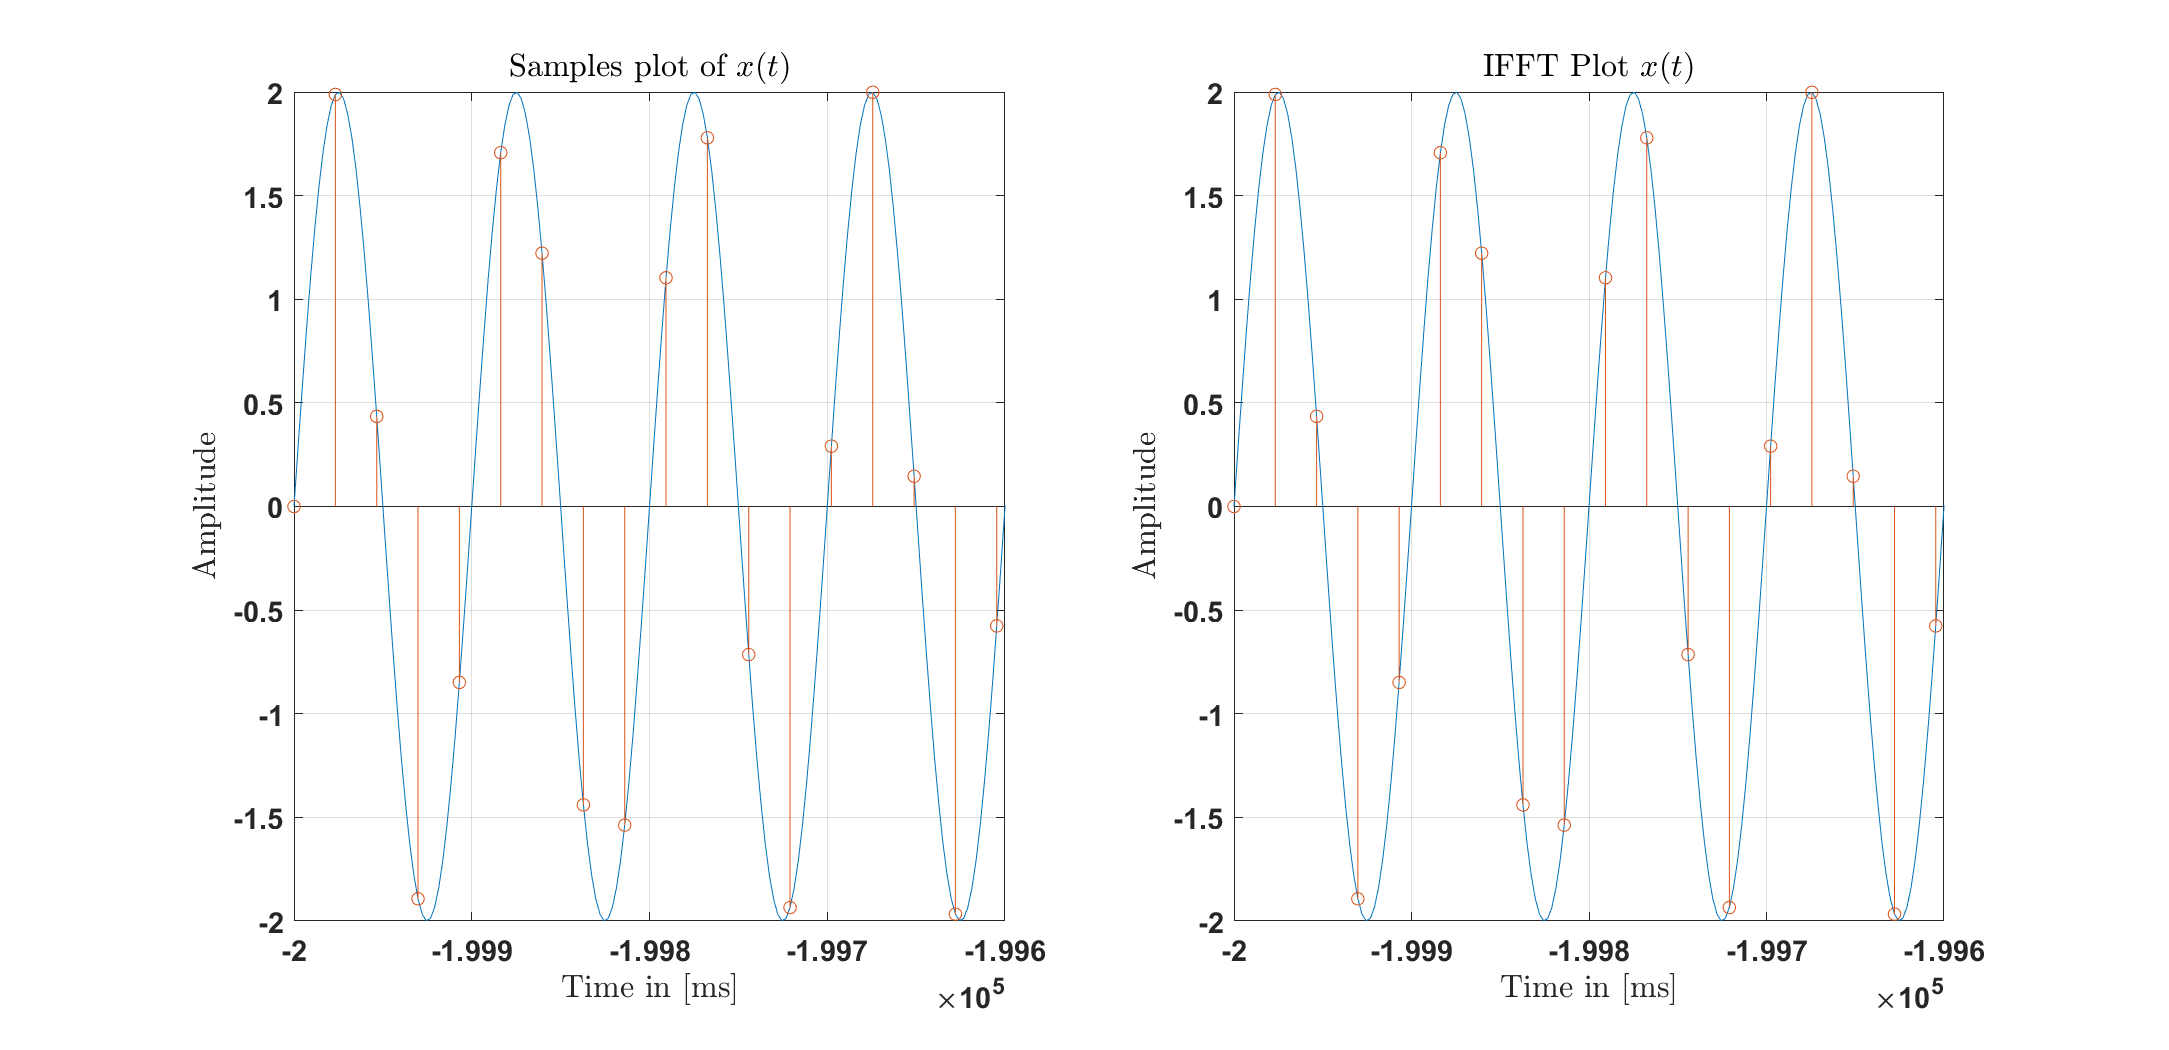
\includegraphics[scale = 0.25]{Figures/Sim_Fourier_Transform/ifft_sin_10_Hz}
\caption{Sin wave where $f \, = \, 10$ Hz}
\label{fig:Sim_Fourier_Transform:ifft_sin_10_Hz}
\end{figure}



\begin{figure}[h]
\centering
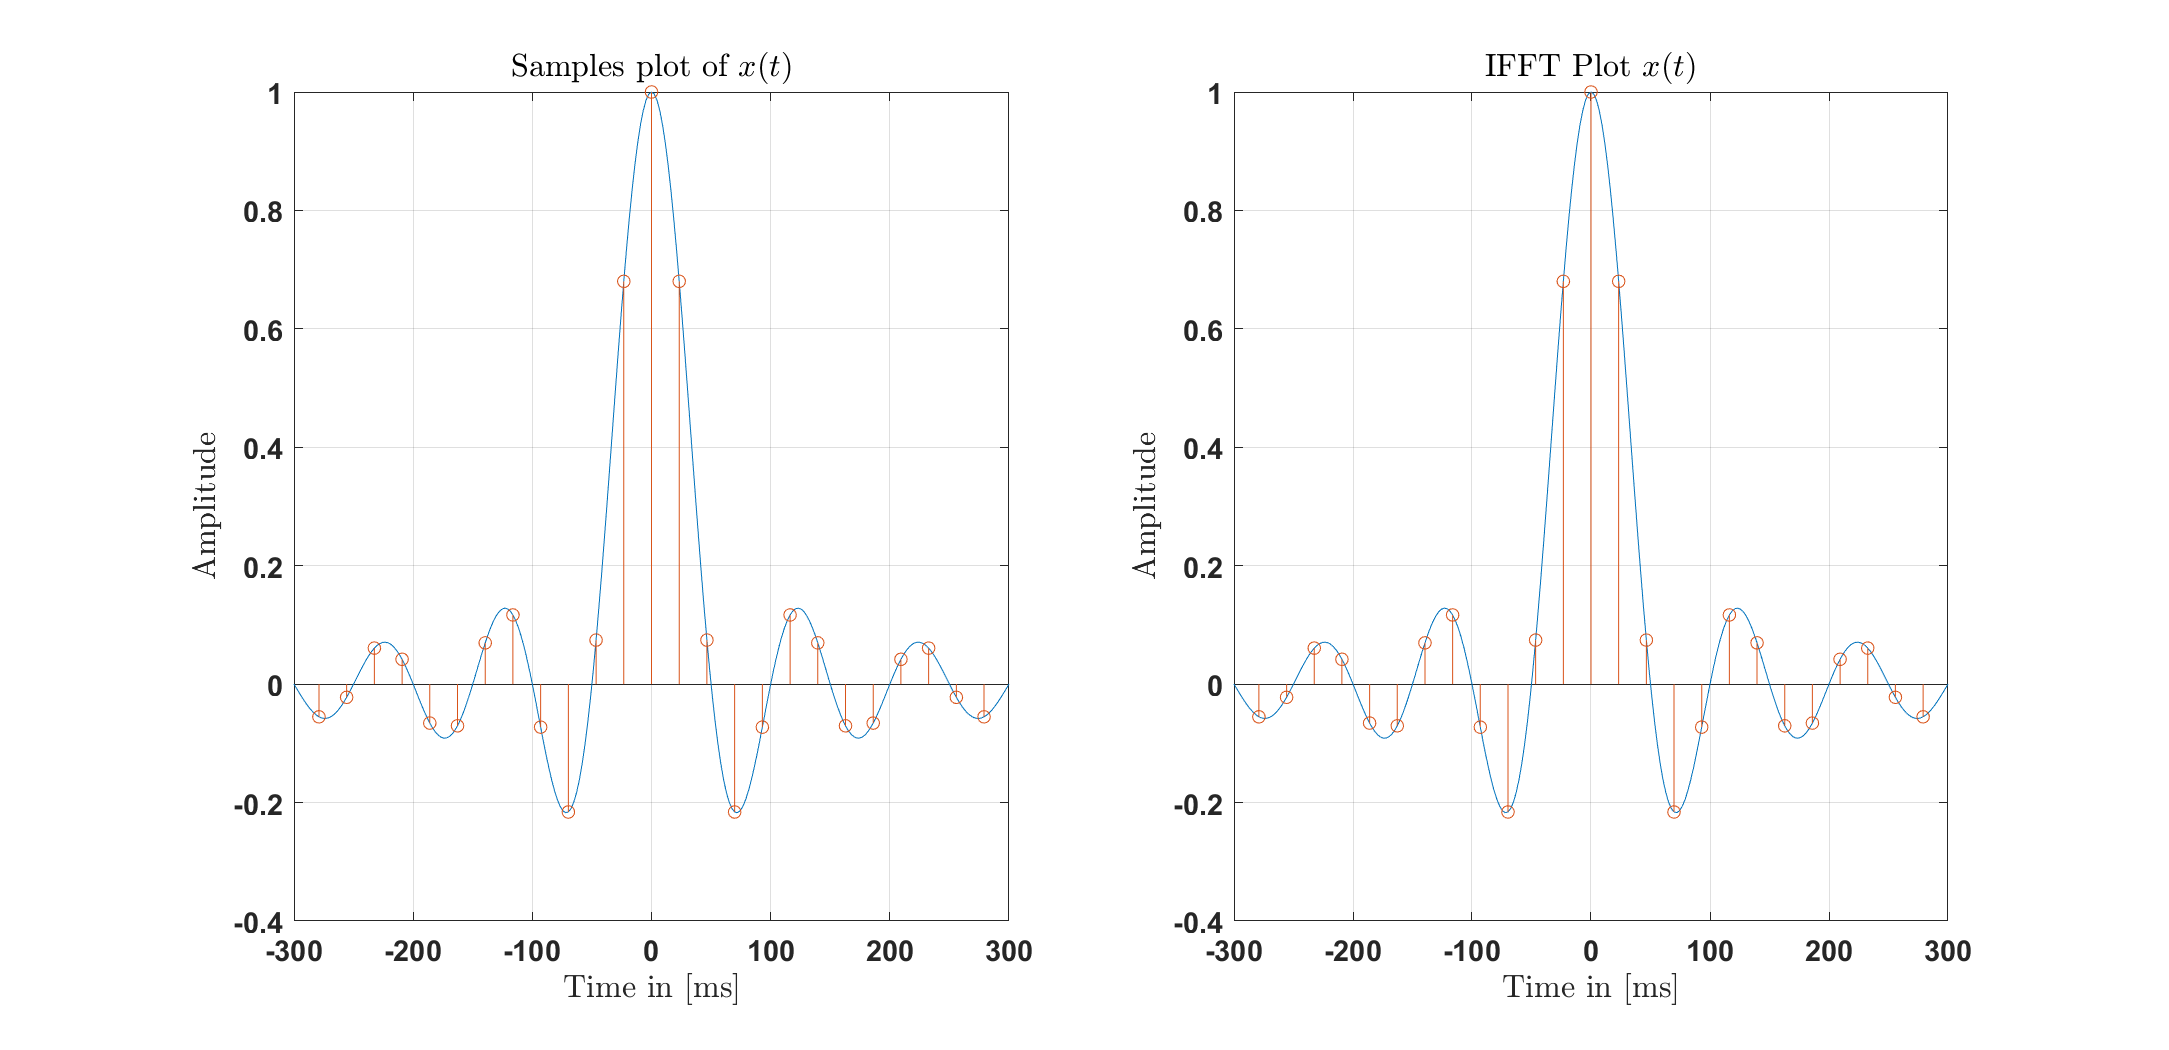
\includegraphics[scale = 0.25]{Figures/Sim_Fourier_Transform/ifft_rect_10_Hz}
\caption{Sinc wave where $B \, = \, 10$ Hz}
\label{fig:Sim_Fourier_Transform:ifft_rect_10_Hz}
\end{figure}

Even if we use zero padding in the \verb|fft|, in the \verb|ifft| we take a length equal to the number of samples (resulting from the uniform sampling process).



\newpage
\section{FFT over Multiple Period}

IN this section, we demonstrate how to plot an FFT spectrum over multiple period.

We all know that usually we plot the FFT from $\displaystyle\frac{-F_s}{2} \rightarrow \, \displaystyle\frac{F_s}{2}$. However, from sampling formula we know that a sampled spectrum is period over multiple of $F_s$.\\


What we can do to implement this periodicity of spectrum is to \tbi{set a new mapping} between the FFT index and the true frequency bin in Hz. This mapping is governed by the relation:


\begin{equation}
    f[\text{Hz}] \, = \, \overbrace{k}^{\text{freq index}}  \, \times \, \overbrace{\displaystyle\frac{F_s}{N}}^{\text{freq step}}
\end{equation}

such that $N \, = \, $ \verb|length-fft|.

A normal spectrum (from $0 \rightarrow F_s$, as the mathematics of DFT says) use the following values of $k$:

\begin{itemize}
    \item $k \, = \, 0 \rightarrow f[\text{Hz}] \, = \, 0$
    
    \item $k \, = \, N \, - \, 1 \rightarrow \, f[\text{Hz}] \, = \, \displaystyle\frac{N \, - \, 1}{N} \, \times \, F_s$
    
\end{itemize}

Then to generate a spectrum centered at 0, we use the \verb|fftshift| command, and the frequency axis using \verb|(-N/2:N/2 - 1) x Fs/N|.\\


Now suppose we want a spectrum from $\displaystyle\frac{-3\, F_s}{2} \rightarrow \, \displaystyle\frac{3 \, F_s}{2}$, the frequency bins generation will be \verb|(-3N/2:3N/2 - 1) x Fs/N|.

\newpage
An output of the simulation is shown in \autoref{fig:Sim_Fourier_Transform:Sinc_B_10Hz_Fs_30_Hz_Multiple_Period}

\begin{figure}[h]
\centering
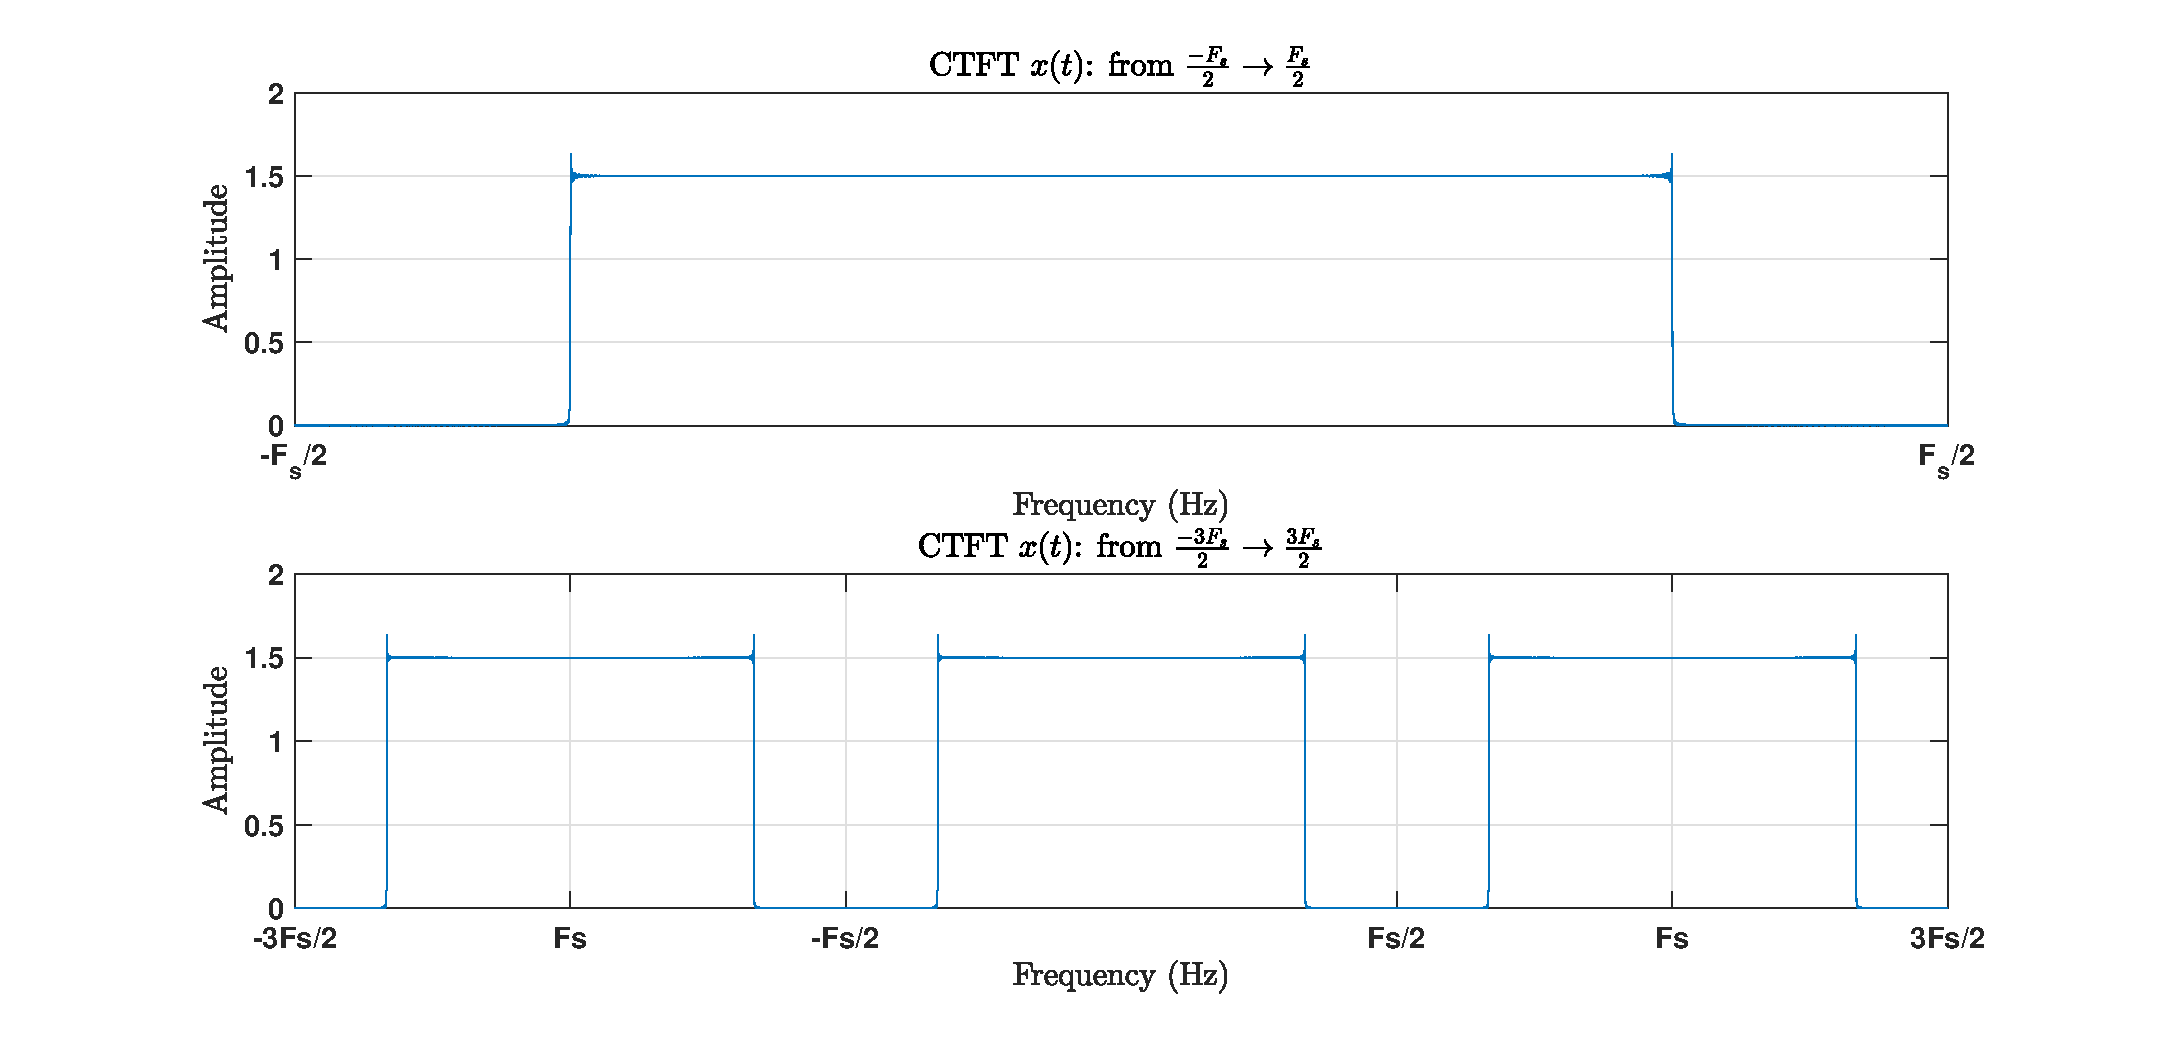
\includegraphics[scale = 0.5]{Figures/Sim_Fourier_Transform/Sinc_B_10Hz_Fs_30_Hz_Multiple_Period}
\caption{Sinc signal where $B \, = \, 10$ Hz and $F_s \, = \, 30$ Hz}
\label{fig:Sim_Fourier_Transform:Sinc_B_10Hz_Fs_30_Hz_Multiple_Period}
\end{figure}

\newpage
\section{Periodic Signals}

In previous section the work was focused on \textit{aperiodic continuous time signal}. Now we turn our attention to periodic signals.

We start with a square wave example, taken from \cite{paper_aliasing_matlab_Sol_Neeman}.

\begin{itemize}
    \item We take fundamental frequency $f_0 \, = \, 30$ Hz $\rightarrow T_0 \, = \, 0.033$s
    
    \item We set the duty cycle to 50 \% $\rightarrow$ in each period, the signal is 50 \% of the time up then down
    
    \item Sampling frequency is set to $F_s = 1$ KHz
    
\end{itemize}

\autoref{fig:Sim_Fourier_Transform:square_wave} shows result of simulation
 
\begin{figure}[h]
\centering
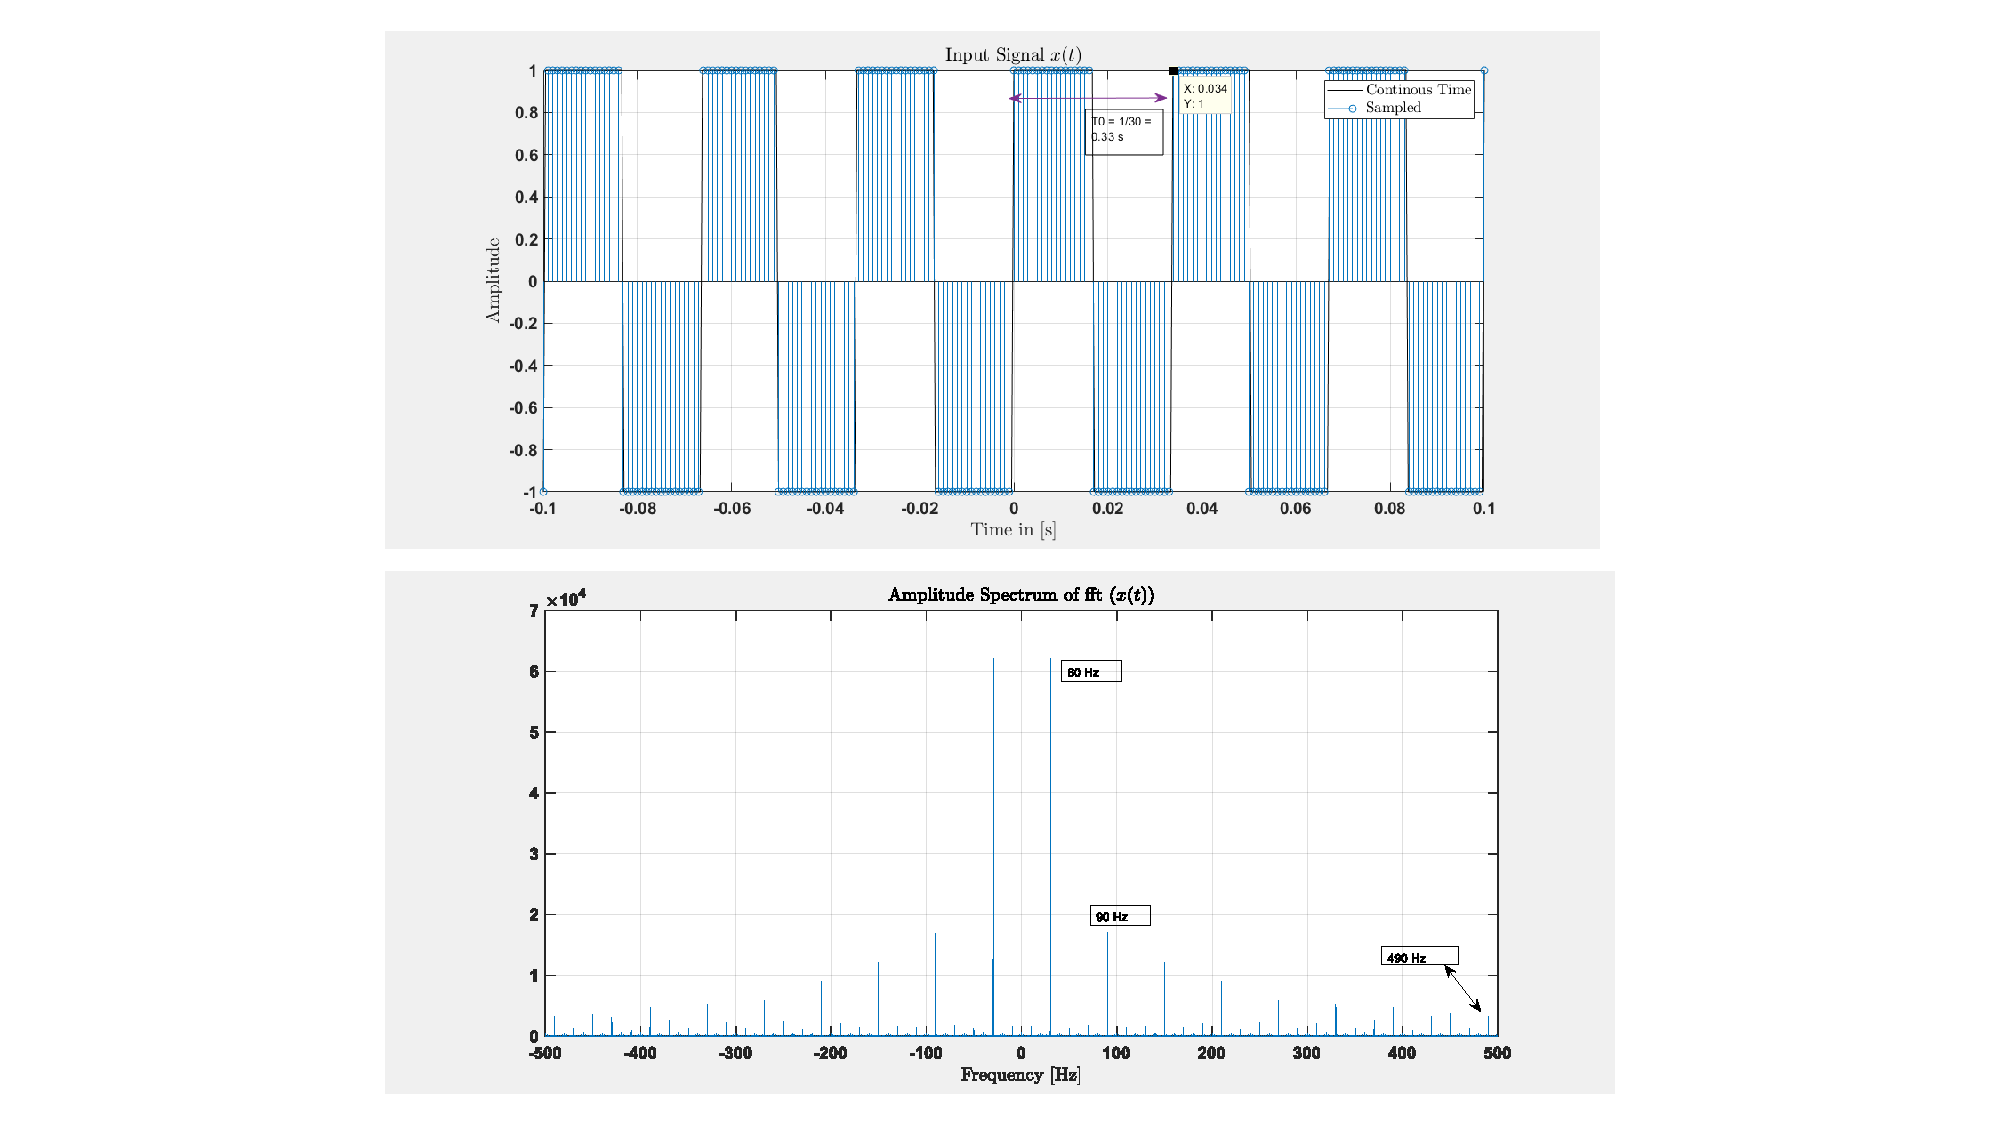
\includegraphics[scale = 0.5]{Figures/Sim_Fourier_Transform/Fourier_periodic_square_wave}
\caption{Square Wave with $F_0 \, = \, 30$ Hz}
\label{fig:Sim_Fourier_Transform:square_wave}
\end{figure}


\begin{itemize}
    \item Fourier Series expression: 
    
    \begin{equation}
        X(t) \, = \, \displaystyle\frac{4}{\pi} \displaystyle\sum_{k = 0}^\infty \displaystyle\frac{\text{sin}\left[ (2 k \, + \, 1) \, 2 \pi f_0 \, t \right]}{(2 k \, + \, 1)}
        \label{Eq:square_wave_fourier_series}
    \end{equation}
    
    
    \item Harmonics appear for odd nature
    
    \begin{itemize}
        \item $k = 0 \rightarrow \, (2k + 1) f_0 =  1 f_0 \, = \, 30$ Hz
        
        \item $k = 1 \rightarrow \, (2k + 1) f_0 =  3 f_0 \, = \, 90$ Hz
        
        \item $k = 2 \rightarrow \, (2k + 1) f_0 =  5 f_0 \, = \, 150$ Hz
        
    \end{itemize}
    
\end{itemize}

\subsection{Aliasing Effect}

It is important to note that the spectrum of doesn't only contains the harmonics, but also \tbi{aliased frequency components}.

Till now, we didn't treat the effect of aliasing in Fourier analysis, since we assume the sampling rate $F_s$ always bigger then the maximum frequency component $f_{\text{max}}$ in the spectrum $\rightarrow F_s > f_{\text{max}}$. (More  treatment to come about this topic in \autoref{Chap:Sampling_Reconstruction}).\\

Here in square wave signal, we don't have a $f_{\text{max}}$ (notice in \autoref{Eq:square_wave_fourier_series} the frequency component keep going to $\infty$). Since $F_s \, = \, 1$ KHz, every frequency component above $\displaystyle\frac{F_s}{2} = 500$ Hz will be aliased to the range of DC $\rightarrow \displaystyle\frac{F_s}{2} = 500$ Hz.

As example, 510 Hz ($k = 17$) will be aliased into 490 Hz as shown in the $\mathrm{2}^\mathrm{nd}$ row of \autoref{fig:Sim_Fourier_Transform:square_wave}.\\

\underline{Aliasing computation:} $490 = F_s \, - 510 = 490$


\newpage
\section{Signals used in Sampling}

\underline{Source:} See section 3.2.3 in \cite{sampling_beyond_band_limited_systems}.

\begin{itemize}
    \item $x(t) \, = \, \delta(t) \, \leftrightarrow \, X(\Omega) \, = \, 1$
    
    \begin{itemize}
        \item For a time shifted dirac: $x(t) \, = \, \delta(t \,- \, t_0) \leftrightarrow \, X(\Omega) \, = \, e^{j \, \Omega \, t_0}$
        
        
        \item Dual transform: 
        
        \begin{itemize}
            \item $x(t) \, = \, 1 \leftrightarrow \, X(\Omega) \, = \, 2 \pi \delta(\Omega)$: constant function (DC component) has its energy only at $\Omega \, = \, 0$ 
            
            \item $e^{j \Omega t_0} \leftrightarrow \, 2 \pi \, \delta(\Omega \, - \, \Omega_0)$: energy contained at $\Omega \, = \, \Omega_0$
            
        \end{itemize}

    \end{itemize}
    
\item Train of Dirac delta function: $x(t) \, = \, \displaystyle\sum\limits_{n \, \in \, \mathbb{Z}} \delta (t \,- \,  n \, T_s)$      


\newpage
\item Rectangular signal: $x(t) \, = \, \begin{cases}
1 \quad \displaystyle\frac{-1}{2} \, \leq t \, \, \leq \displaystyle\frac{1}{2} \\
0 \quad \text{otherwise}
\end{cases} \leftrightarrow \, X(\Omega) \, = \, \text{sinc}\left(\,  \displaystyle\frac{\Omega}{2 \pi}  \, \right)$

\begin{itemize}
    \item Dual transform and using time scale property: $\text{sinc}\left(\,  \displaystyle\frac{t}{T}  \, \right) \, \leftrightarrow \, X(\Omega) \, = \, T$ for $ \displaystyle\frac{-\pi}{T} \, \leq  \, \Omega \, \leq \,  \displaystyle\frac{\pi}{T}$ 
\end{itemize}

\begin{figure}[h]
\centering
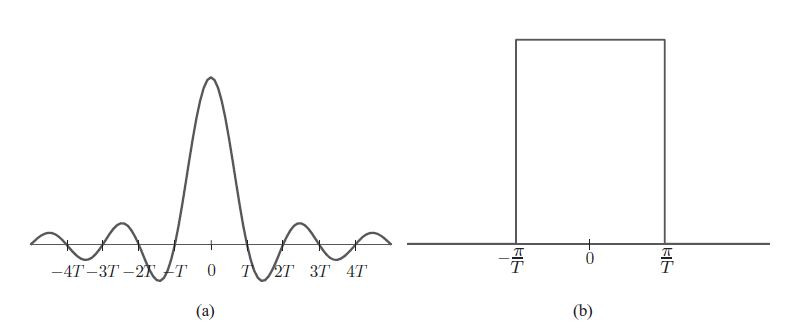
\includegraphics[scale = 0.5]{Figures/Sim_Fourier_Transform/sinc_rect_Fourier}
\caption{CTFT of $\text{sinc}\left(\,  \displaystyle\frac{t}{T}  \, \right)$ \cite{sampling_beyond_band_limited_systems}}
\label{fig:Sim_Fourier_Transform:sinc_rect_Fourier}
\end{figure}


\item Discrete Exponentials (section 3.3.2 in \cite{sampling_beyond_band_limited_systems}):

\begin{equation}
    x[n] \, = \, e^{j \, \omega_0 \, n} \leftrightarrow \, X(\omega) \, = \, 2 \pi \displaystyle\sum_{k \, \in \, \mathbb{Z}} \delta(\omega \, - \, \omega_0 \, + \, 2 \,  \pi \, k)
\end{equation}
    
\end{itemize}


\newpage
\section{Continuous–discrete Representations}

\underline{Source:} See section 3.2 in \cite{sampling_beyond_band_limited_systems}.\\

In context of sampling, we deals with a \tbi{mixed signal representation}, involving 2 components: a continuous time signal $x(t)$ and a discrete time sequence $d[n]$, having the form:


\begin{equation}
    x(t) \, = \, \displaystyle\sum_{n \in \mathbb{Z}} d[n] \, h(t \, - \, n \, T_s)
\end{equation}

Some facts:

\begin{itemize}
    \item $X(\Omega) \, = \, D(\omega) \, H(\Omega)$
\end{itemize}



%****************************************
%****************************************
%****************************************



\chapter{\texorpdfstring{$Z$}{Z}-Transform}

\section{Polynomial Manipulation}

Polynomial are encountered in $z$-transform allot.\\

Suppose we have the following polynomial $P(z) \, = \,1 z^0 + 1.5 z^{-1} + 2 z^{-2}$. We can do 3 type of manipulation:

\begin{enumerate}
    
\item Compute the root using the function \verb|root|

\item Compute the polynomial coefficient from the root using \verb|poly(root)|

\item Evaluating a polynomial at some value of $z$ using function \verb|polyval|

\end{enumerate}


\section{Partial Fraction Expansion}

Example:

\begin{equation}
\begin{array}{rcl}
    X(z) \, &=& \, \displaystyle\frac{6 \, - \, 10 \, z^{-1} \, 2 \, z^{-2}}{1 - 3 z^{-1} + 2 z^{-2}}  \\ \\
     &=& \, 1 \, + \,  \displaystyle\frac{2}{1 \, - \,z^{-1} } \, + \, \displaystyle\frac{3}{1 \, - \,2 \, z^{-1}}
\end{array}    
\end{equation}

In general, $X(z)$ can be written as:

\begin{equation}
\begin{array}{rcl}
X(z) \, &=& \, \displaystyle\frac{B(z)}{A(z)}   \, = \, \displaystyle\frac{b_0 \, + \, b_1 \, z^{-1} \, + \, \cdots \, + \, b_M \, z^{- \, M}}{a_0 \, + \, a_1 \, z^{-1} \, + \, \cdots \, + \, a_N \, z^{- \, N}} \\ \\
	    &=& \, \displaystyle\sum\limits_{i \, = \, 1}^{M \, - \, N} C_i \, z^{-i} \, + \,  \displaystyle\sum\limits_{i \, = \, 1}^N\frac{A_i}{1 \, - \, p_i \, z^{-1}}
 \end{array}
\end{equation}

If $M< \, N$ (proper rational function) $\rightarrow \, C_i \, = \, 0$.\\

\newpage
In the example:

\begin{itemize}
    \item poles $= \, [1 \, ; \,  2]$
    
    \item $A \, = \, [2 \, ; \, 3]$
    
    \item $C \, = \, 1$ since $M \, = \, N \, = \, 2$
    
\end{itemize}

This implemented \verb|[terms,poles,num_constants] = residuez(coeff_num,coeff_deno)|.


\section{Zero-Pole Pattern}

Consider the system defined as

\begin{equation}
  H(z) \, = \, \displaystyle\frac{1 \, -  \, z^{-2}}{1 \, + \,  0.9 z^{-1} \, + \,  0.6 z^{-2} \, + \, 0.05 z^{-3}} 
\end{equation}

This is a $\mathrm{3}^\mathrm{rd}$ order system where $M \, = \, 2$ and $N \, = \, 3$.\\

To plot the zero-pole pattern in $z$-plane, we use the function \verb|zplane(coeff_num,coeff_deno)|.\\

\subsection{Impulse Response}

We can also plot the impulse response numerically using the function \verb|impz(coeff_num,coeff_deno,number_samples)|. If the system is stable, $h[k]$ will tend for 0 asymptotically. 

\section{Inferring Frequency Response}

When evaluating frequency response from $H(z)$, we choose several value of $z$ on the unit circle. This means that the ROC must include the unit circle so we can do this evaluation.\\

Usually $H(z)$ expression comes in the form of rational fraction.

\begin{enumerate}

\item $\mathrm{1}^\mathrm{st}$ order system: $h[k] \, = \, \left( \displaystyle\frac{1}{3} \right)^k \, u[k] \, \mapsto \, H(z) \, = \, \displaystyle\frac{1}{1 \, - \, \frac{1}{3} \, z^{-1} } \, $, such that its ROC : $\lvert z \rvert \, > \, \displaystyle\frac{1}{3}$.

We have a zero $\, = \, 0$ and pole at $\frac{1}{3}$.\\

Recall that a rational transfer function can be written as

$H(\omega_d) \, = \, \displaystyle\frac{\prod \text{Length of the Vector away from 0}}{\prod \text{Length of the Vector away from poles}}$.\\

When evaluting $H(\omega_d)$ on the unit circle, the vector from 0 remains constant as we move around (because the zero it is on the origin), and the vector of the pole change.\\

The pole vector will increase when we move $\omega_d$ from $0 \, \rightarrow \, \pi$, which means that the ratio will decrease. We can say that because the length of the zero vector is constant, and hence we expect a LPF behavior.
    
    

\item $\mathrm{2}^\mathrm{nd}$ order system: $h[k] \, = \, \left( \displaystyle\frac{5}{6} \right)^k \, \sin{ \left( \displaystyle\frac{\pi}{3} \, k \right)} \, u[k] \, \mapsto \, H(z) \, = \, \displaystyle\frac{\displaystyle\frac{5}{6} \, \sin{ \left( \displaystyle\frac{\pi}{3} \, \right)} \, z^{-1}  }{1 \, - \, \displaystyle\frac{10}{6}  \, \cos{ \left( \displaystyle\frac{\pi}{3} \, \right)} \,   z^{-1} \, + \,  \left(\, \displaystyle\frac{5}{6} \, z^{-2} \, \right)^2} \, $.\\

In this system we have a complex conjugate poles, having the following polar coordinates: radius $= \, \displaystyle\frac{5}{6} $ and angle $ \displaystyle\frac{\pi}{3}$.


As we move toward high frequency components, so away from $ \displaystyle\frac{\pi}{3}$, the distance from the poles to unit circle increase $\leftrightarrow$ influence of the poles increase $\leftrightarrow \, \lvert H(\omega_d) \rvert$ decrease.\\

Now taking the opposite direction, by moving toward low frequency components $\leftrightarrow$ from $ \displaystyle\frac{\pi}{3} \, \rightarrow \, 0$, the poles vector (from the poles to the unit circle) decrease, so $\leftrightarrow \, \lvert H(\omega_d) \rvert$ is larger.\\


\underline{Influence of the radius to the Poles}

If we decrease the radius, the location of the poles will push down further to the origin (further away from the unit circle), and hence we will loose the band pass effect at $\displaystyle\frac{\pi}{3}$.

    
    
    
\end{enumerate}


\chapter{Windowing and Spectral Analysis}
\label{Chap:Windowing}

\underline{\textcolor{purple}{References}:} based on section 7.6 in \cite{DSP_DimitrisManolakis} and section 4.9 in \cite{signal_processing_Lathi}\\

DFT (or FFT) are the computational tools which can approximate any type of Fourier transform (CTFT, CTFS,$\cdots$).

The problem of computing the DFT is always done by passing through 3 fundamental steps:

	\begin{enumerate}
	\item Sample the continuous-time signal
	
	\item Select a finite number of samples for analysis
	
	\item Compute the spectrum at a finite
number of frequencies (frequency sampling)
	\end{enumerate}

Truncation is always done in real time signal processing since we have a limited amount of memory to store and process signals.\\

Focus in this section:effects of the \tbi{selection of a finite-length segment of the sampled signals}, because it
has the biggest impact on the accuracy of the estimated spectrum.\\

\underline{Assumption to be done during the analysis:}  the signal is sampled correctly in the time domain $\leftrightarrow$ effects of aliasing are negligible.


\section{Modeling the problem of truncation}

\begin{itemize}

\item Selecting a finite number of samples in the signal $\leftrightarrow$ multiplying the signal with some window

\item Multiplying in the time domain $\leftrightarrow$ convolution in the frequency domain

\item We consider first a \textcolor{red}{rectangular window using simple cos signals}, then make the analysis for other choices


\item Mathematical equations:

\begin{equation}
x_w(t) \, = \, x(t) \, \times \, w(t) \leftrightarrow \, X_w(F) \, = \, X(F) \, \star \, W(F)
\end{equation}

\newpage
\item Analysis by inspection: if we take $\Pi \left(\, \displaystyle\frac{t}{\tau} \,\right) \, \leftrightarrow \, \tau \,  \text{sinc} \left(\, \pi \,F \,  \tau \,  \right)$

	\begin{itemize}
	\item Main lobe width $= \, \displaystyle\frac{4 \pi}{\text{duration}}$ (see figure \autoref{fig:DFT:amp_spec_rect_window})
	
	\item Convolution of 2 signals: shifting and adding the 2 signals up
	
	\item So if we have some frequency content in our signal, it will be added up (\tbi{signal will be blurred}) in the main lobe of the sinc
	\end{itemize}


\begin{figure}[ht]
\centering
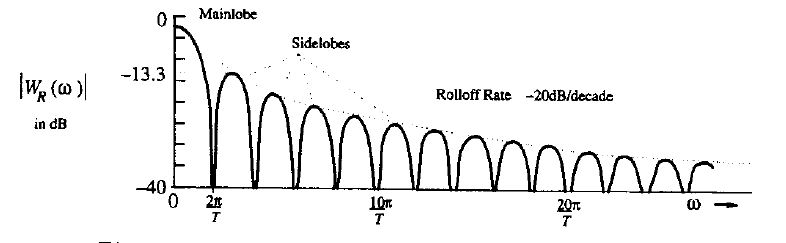
\includegraphics[scale=0.6]{Figures/DFT/amp_spec_rect_window}
\caption{Amplitude Spectrum for Rectangular Window \cite{signal_processing_Lathi}}
\label{fig:DFT:amp_spec_rect_window}
\end{figure}

\end{itemize}

\underline{Example: Effect of Window with a cos Signal}

\begin{itemize}

\item Let $x(t) \, = \, A_1 \, \cos( 2 \pi f_0 \, t \, + \, \phi)$

\item The spectrum of $x(t)$ can be directly obtained using Euler identity

\begin{equation}
    x_c(t) \, = \, \displaystyle\frac{1}{2} \, A_1 \, e^{-j \, \phi} \, e^{-j \,2 \pi f_0 \, t} \, + \, \displaystyle\frac{1}{2} \, A_1 \, e^{j \, \phi} \, e^{j \, 2 \pi f_0 \, t}
\end{equation}


\item The time windowed signal $x_w(t)$:

\begin{equation}
 x_w(t) \, = \, \displaystyle\frac{1}{2} \, A_1 \, e^{-j \, \phi} \, w(t) \, e^{-j \, 2 \pi f_0 \, t} \, + \, \displaystyle\frac{1}{2} \, A_1 \, e^{j \, \phi} \, \, w(t) \, e^{j \, 2 \pi f_0 \, t} 
 \label{Eq:DTF:Window_Eq_1}
\end{equation}

\item Taking the CTFT of \autoref{Eq:DTF:Window_Eq_1} and using the frequency shift property \cite{signal_processing_Lathi} ( $x(t) \, e^{j \, 2 \pi f_0 \, t} \leftrightarrow \, X(F \, - \, f_0)$ ), we have:

\begin{equation}
   X_w(F) \, = \, \displaystyle\frac{1}{2} \, A_1 \, e^{-j \, \phi} \, W(\, F \, + \, f_0 \,)  \, + \, \displaystyle\frac{1}{2} \, A_1 \, e^{j \, \phi} \, \, W(\, F \, - \, f_0 \,)
 \label{Eq:DTF:Window_Eq_2}  
\end{equation}

\item Interpretation of \autoref{Eq:DTF:Window_Eq_2}: the effect of time windowing is to replace each spectral line of the CTFT spectrum with \tbi{scaled copy of}  $W(F)$ centered at the frequency  of the line

\item As an example of a window, we begin with a rectangular one: 

\begin{equation}
\Pi \left(\, \displaystyle\frac{t}{\tau} \,\right) \, \leftrightarrow \, \tau \,  \text{sinc} \left(\, \pi \,F \,  \tau \,  \right)    
\end{equation}


\newpage
\item Visualisation of the computation steps are shown in \autoref{fig:DFT:windowing_modeling_2}

\begin{figure}[ht]
\centering
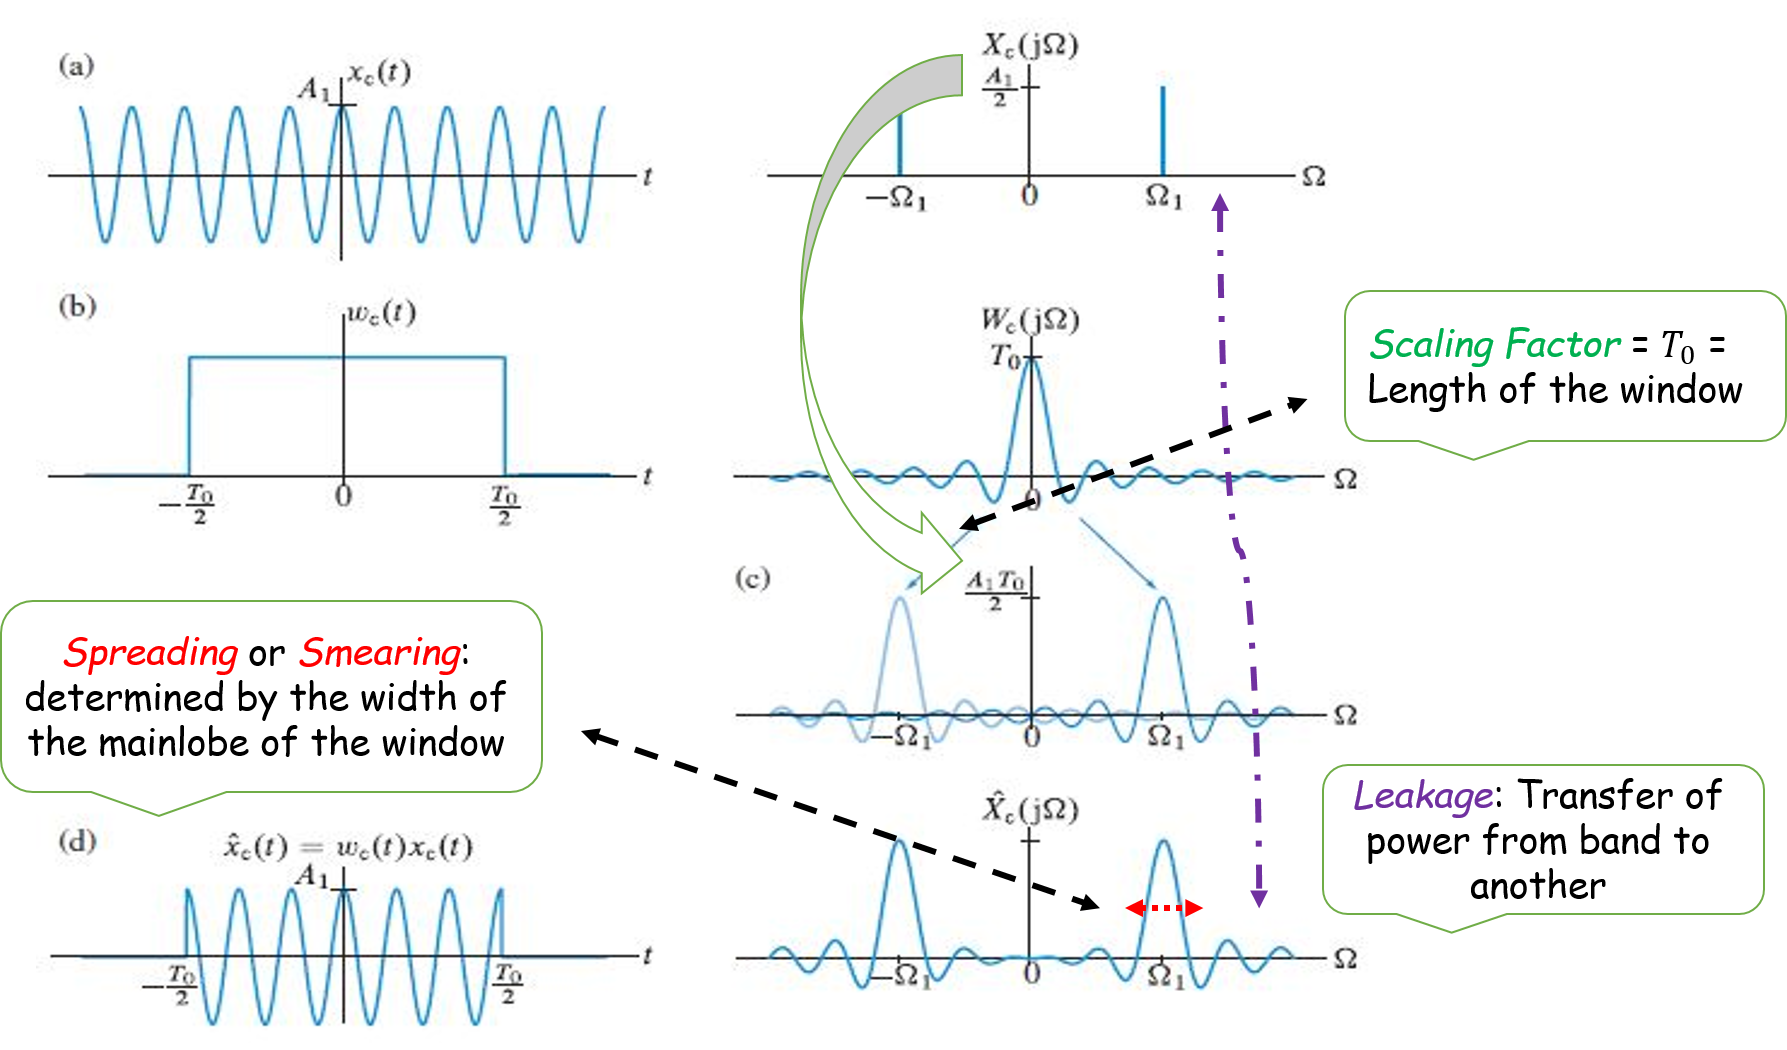
\includegraphics[width = 0.80\textwidth]{Figures/DFT/windowing_modeling_2}
\caption{Windowing Effect on CTFT Amplitude Spectrum}
\label{fig:DFT:windowing_modeling_2}
\end{figure}


3 Things to be noticed from figure \autoref{fig:DFT:windowing_modeling_2} \cite{DSP_DimitrisManolakis}

\begin{enumerate}

\item \tbi{Spectral Spreading} or \tbi{Spectral Smearing}

	\begin{itemize}
	
	\item Controlled by the \tbi{width of the main lobe}	
	
	\item The cosine signal now has spread out after and before $\omega_{c_1}$
	
	\item Smearing can cause \tbi{peak merging }$\leftrightarrow$ reduce the resolvability in the spectrum when have several components close to each other
	
		\begin{itemize}
		\item To be seen in the simulations after
		\end{itemize}
		
	\end{itemize}


\item \tbi{Leakage}:

	\begin{itemize}
	
	\item Controlled by the \tbi{sidelobs} of the rectangular window	
	
	\item Leakage create false peaks due to the power transfer
	
	\item Also it hides any weak frequency components as we will see in the simulation results after
	\end{itemize}


\item Also notice that the amplitude spectrum is multiplied by $T_0$, the length of the window

	\begin{itemize}
	\item This is because the rect window amplitude spectrum has a maximum equal to $T_0$
	\end{itemize}

\end{enumerate}

\end{itemize}

\newpage
\section{Simulation Rectangular Window}

First we simulate a DTFT of a rectangular window for different length.

\begin{figure}[ht]
\centering
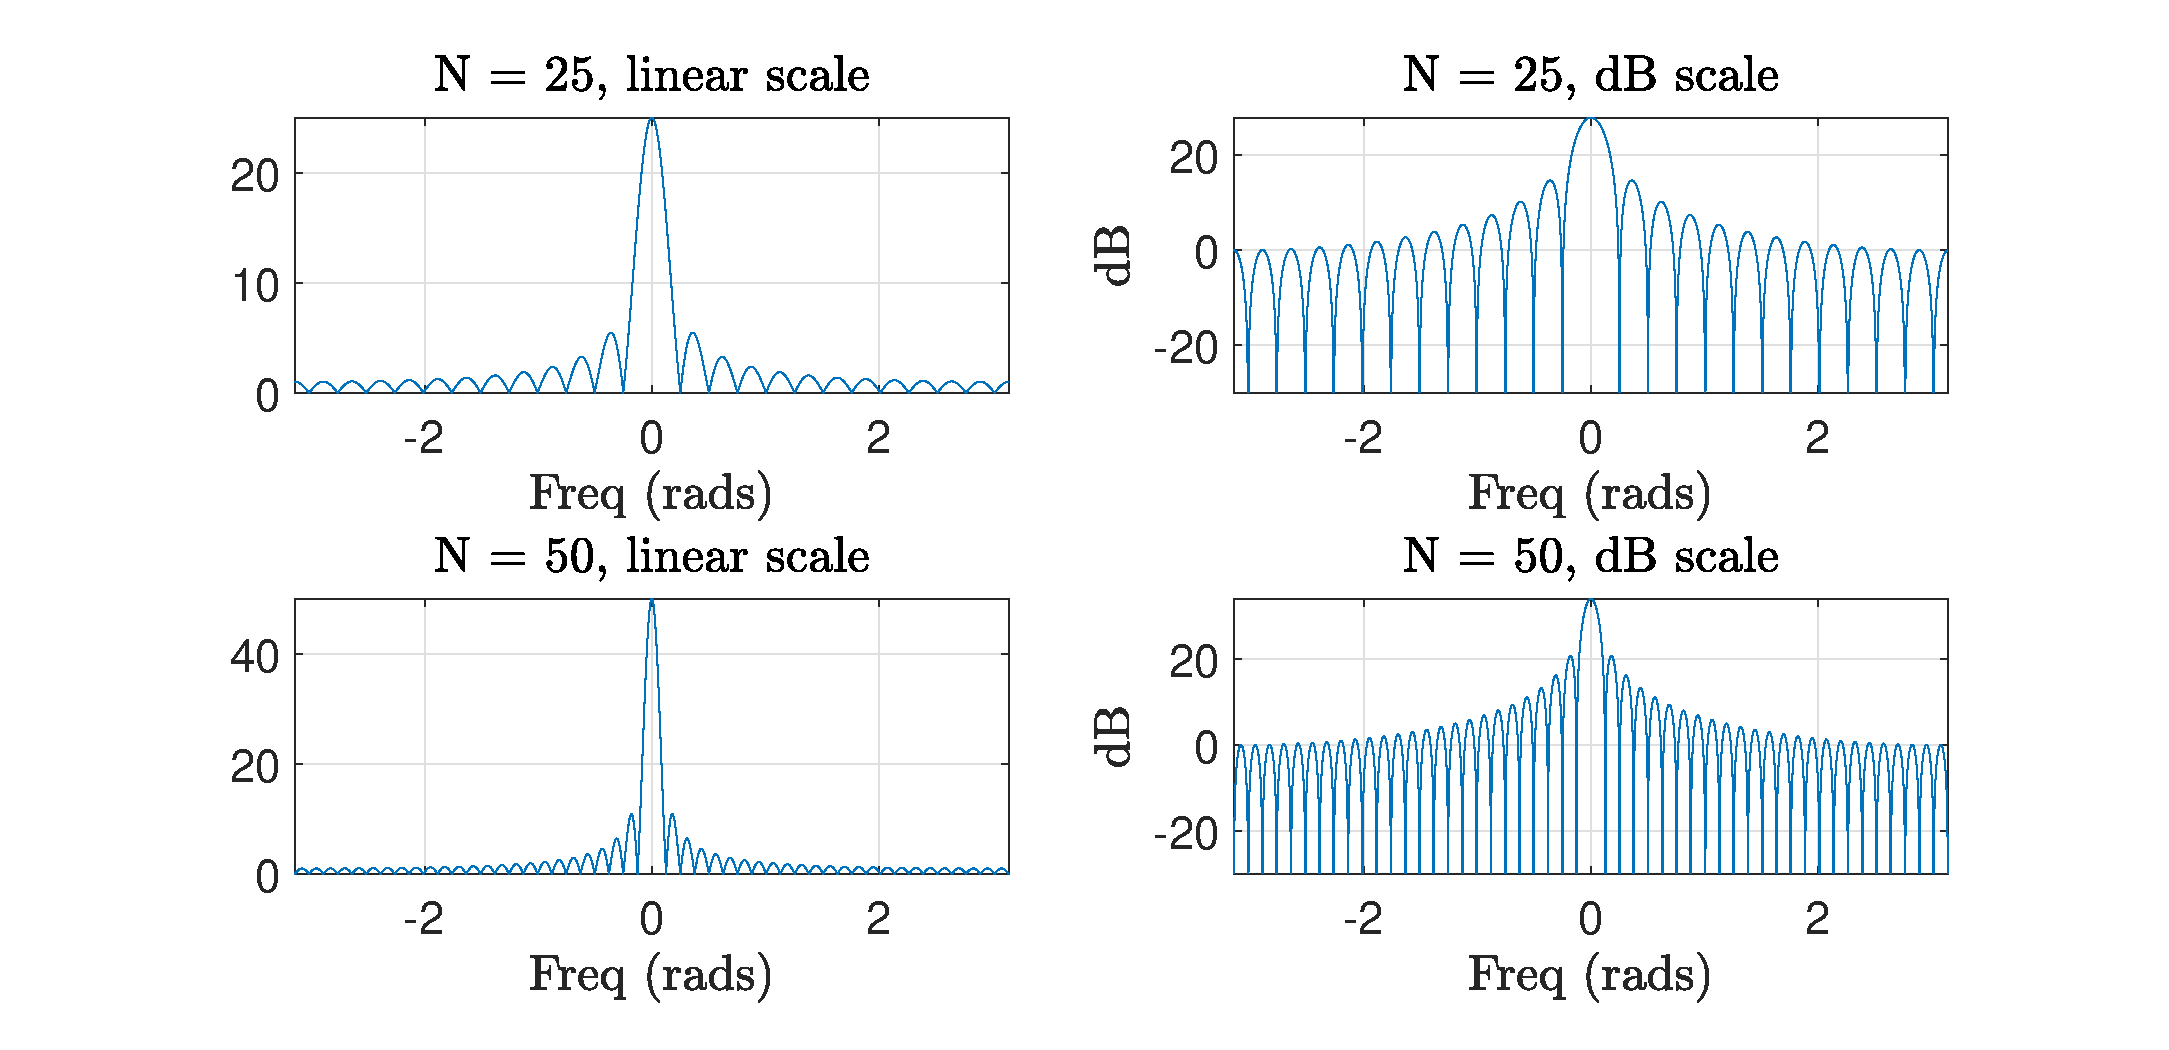
\includegraphics[scale = 0.3]{Figures/Simulation_Sampling_Frequency_Analysis/rect_window_nb_samples}
\caption{DTFT Amplitude Spectrum for the Rectangular Window in Linear and dB Scale}
\label{fig:Simulation_Sampling_Frequency_Analysis:rect_window_nb_samples}
\end{figure}


if we choose \tbi{higher number of samples}

\begin{enumerate}
\item We get a \tbi{narrower main lobe}
	
\item But the \tbi{side lobes doesn't change that much}
\end{enumerate}


\section{Simulation 2 Cos Signals}

If the \tbi{cosine signals are too close together}, then doing convolution with our window will add up the 2 cos, and hence we can't distinguish the frequency content of the signals
	
		\begin{itemize}
		\item This is known of \textcolor{red}{peak merging} (loss of spectral resolution) when the 2 spectral line are closer then the width of the main lobe \cite{DSP_DimitrisManolakis}
		\end{itemize}

\begin{figure}[ht]
\centering
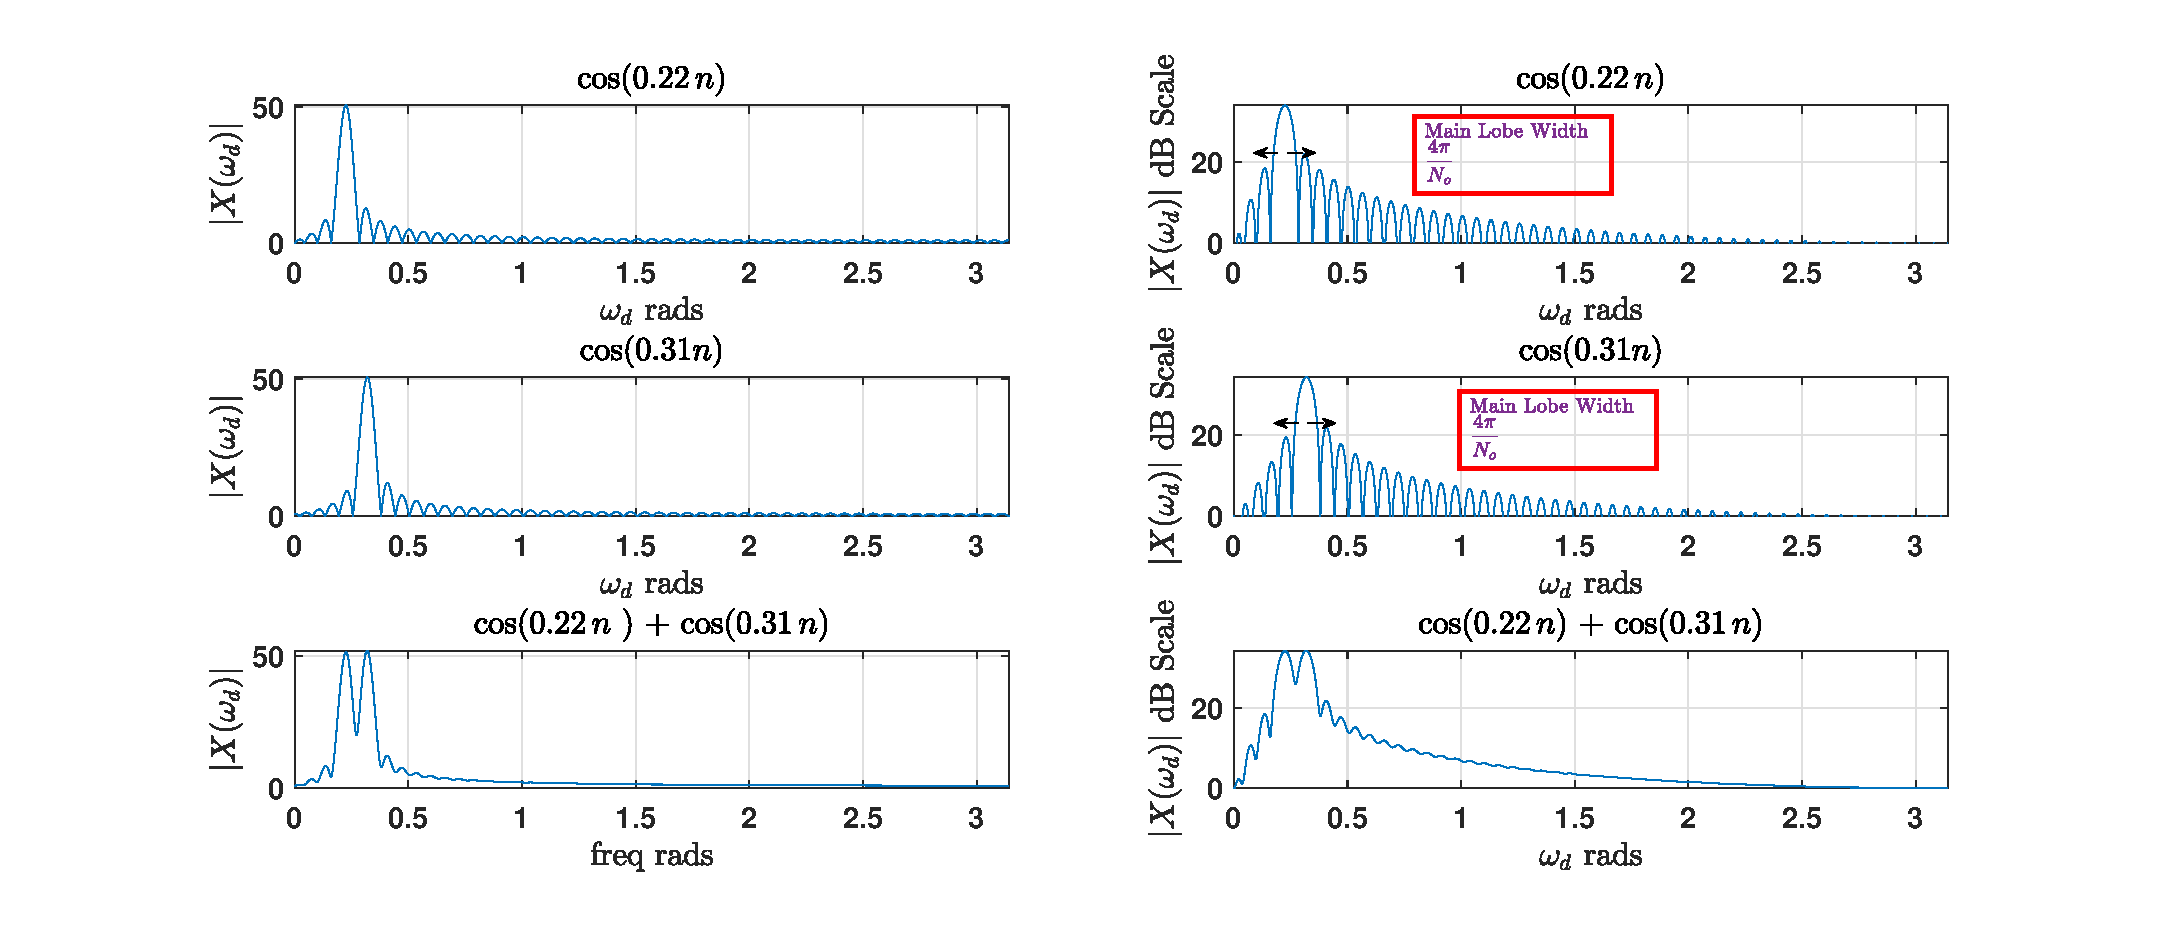
\includegraphics[width = 1\textwidth]{Figures/DFT/spaced_cos}
\caption{Spaced Cos signal}
\label{fig:DFT:spaced_cos}
\end{figure}

\begin{itemize}

\item We have 2 cos signals with discrete frequencies:

	\begin{itemize}
	\item $ \omega_{d_1} \, = \, \displaystyle\frac{7 \pi}{100} \approx \, 0.22$ and $ \omega_{d_2} \, = \, \displaystyle\frac{10 \pi}{100} \approx \, 0.31$ 
	
	
	\end{itemize}

\item Width of the main lobe $ = \displaystyle\frac{4 \pi}{N} \, = \, \displaystyle\frac{4 \pi}{100}$

	\begin{itemize}
	\item Where $N$ is the length of the rectangular window
	\end{itemize}

\item Spectral separation between signals $= \displaystyle\frac{10 \pi}{100} \, - \, \displaystyle\frac{7 \pi}{100} \, = \, \displaystyle\frac{3 \pi}{100}$

\item Separation rule: Width of the main lobe $\leq$ Spectral separation between signals $\leftrightarrow \,\displaystyle\frac{4 \pi}{100} \,\leq \,  \displaystyle\frac{3 \pi}{100} \, \leftrightarrow$ rule is almost verified with some errors however

	\begin{itemize}
	\item  But still we are able to distinguish the 2 components
	\end{itemize}
	
\end{itemize}

\underline{1 Weak and 1 Strong Signal}\\

Trickiest part: don't forget \tbi{the side lobes}

\begin{itemize}
	
\item Case of 1 strong and the $\mathrm{2}^\mathrm{nd}$ is weak
	
\item Even if the $\mathrm{2}^\mathrm{nd}$ component is far from the $\mathrm{1}^\mathrm{st}$ one, the $\mathrm{2}^\mathrm{nd}$ could be a small one and add up with the side lobes of the $\mathrm{1}^\mathrm{st}$ one (the strong one)

\end{itemize}


\begin{figure}[ht]
\centering
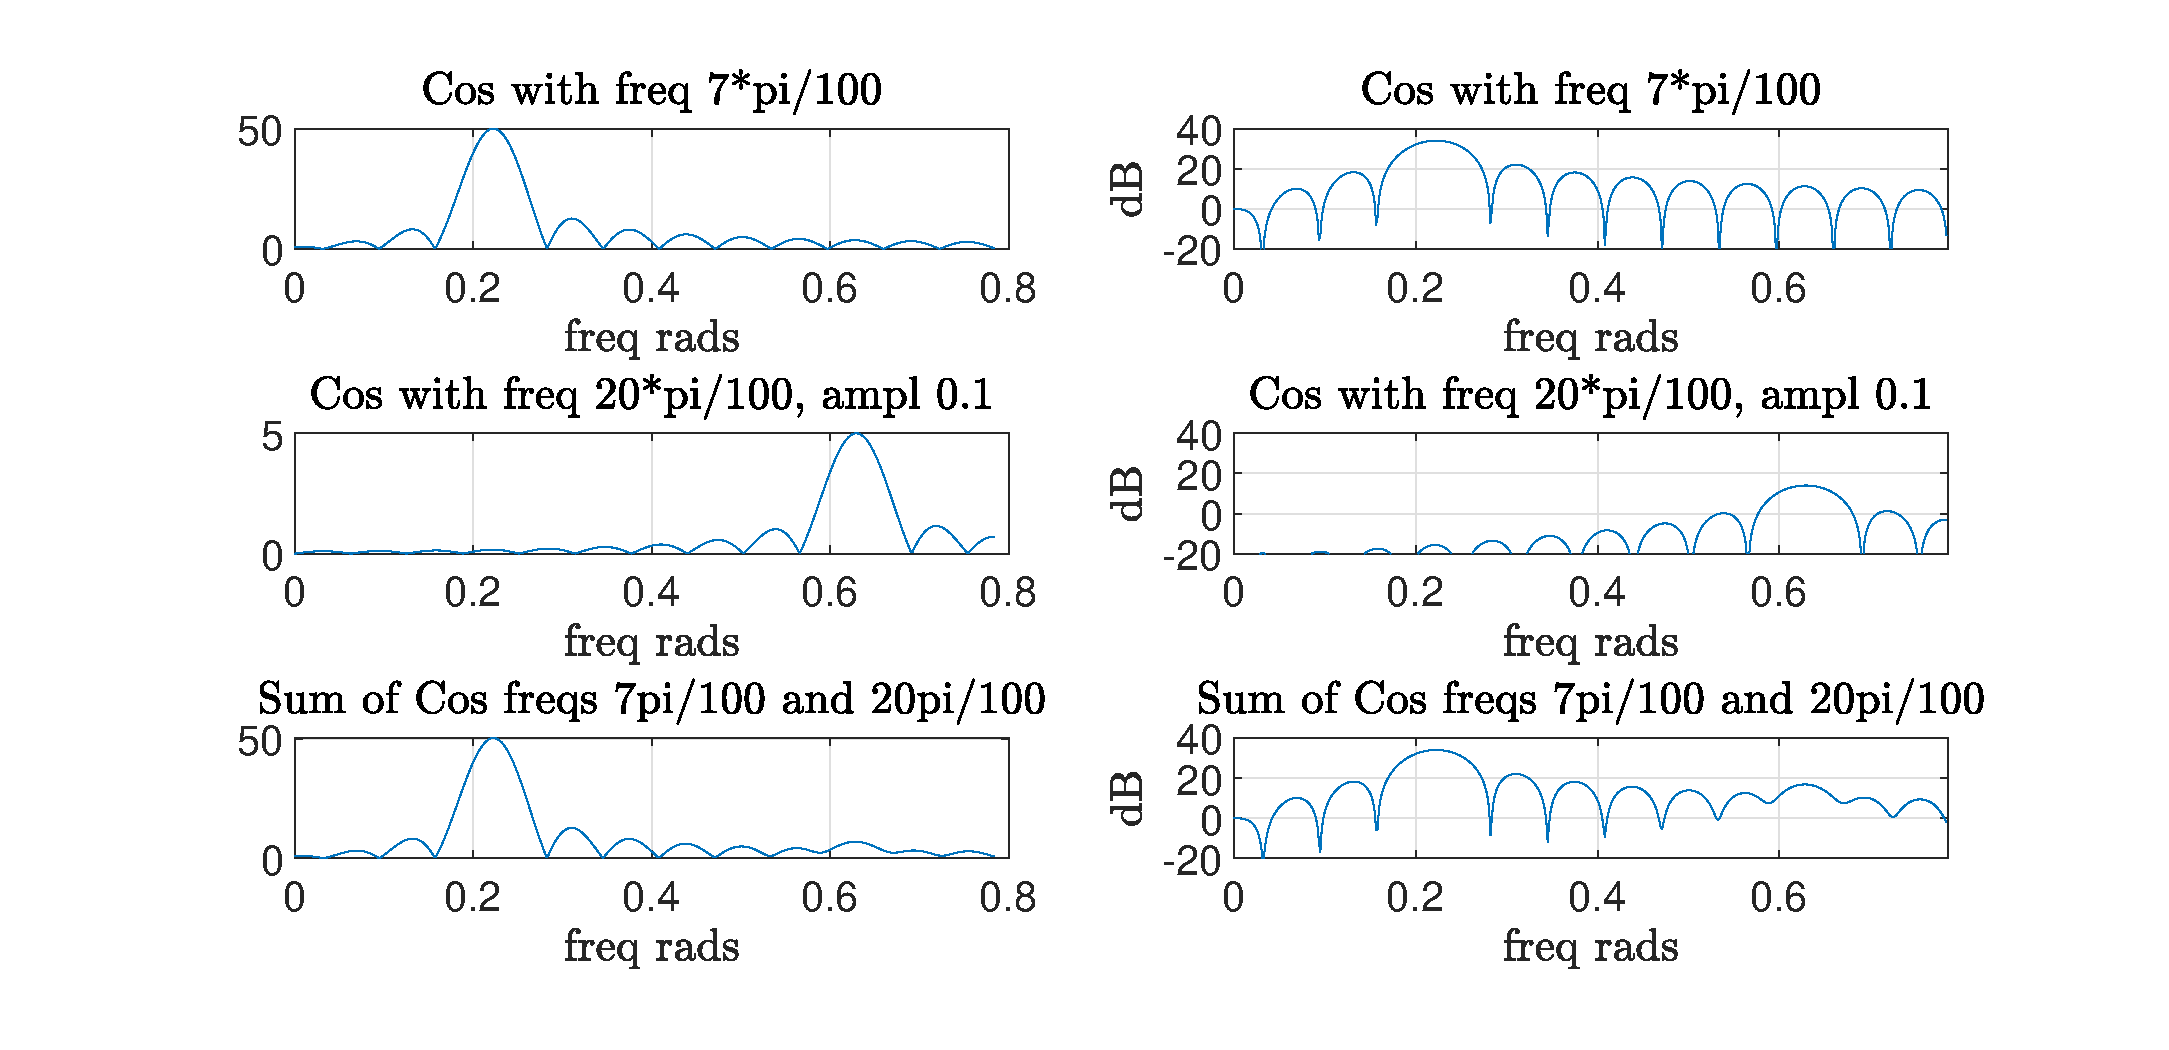
\includegraphics[width = 1\textwidth]{Figures/Simulation_Sampling_Frequency_Analysis/spaced_weak_cos}
\caption{Well separated signals but with weak components}
\label{fig:Simulation_Sampling_Frequency_Analysis:closed_cos}
\end{figure}

\section{Window Choice}

\begin{itemize}

\item In previous part, we have seen the effect of side lobs in a rectangular window:

	\begin{enumerate}
	\item Very high resolution $\leftrightarrow$ narrow main lobe
	
	\item Not very efficient dynamic range $\leftrightarrow$ side lobe effects still high even if we truncate less
	\end{enumerate}


\item In rectangular window, we have a sudden transition from $1 \rightarrow 0$ or $0 \rightarrow 1$ in the time domain, which make the side lobes to be appear in the frequency domain (in CTFT or DTFT Spectrum)

\item This was the motivation for designing other choices of windows: \tbi{trade-off between resolution and dynamic range}

\item Design criteria for \tbi{good window}: 

	\begin{enumerate}
	\item Narrow mainlobe
	
	\item Weak side lobes
	\end{enumerate}


\item Different Window Types

\begin{figure}[ht]
\centering
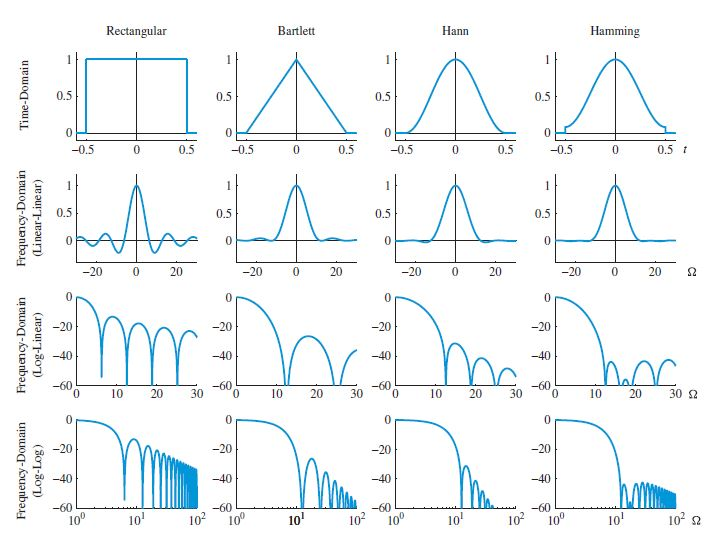
\includegraphics[scale=0.4]{Figures/DFT/other_windows}
\caption{Time-domain and frequency-domain characteristics of continuous-time rectangular, Bartlett (triangular), Hann, and Hamming windows \cite{DSP_DimitrisManolakis}}
\label{fig:DFT:other_windows}
\end{figure}


\begin{figure}[ht]
\centering
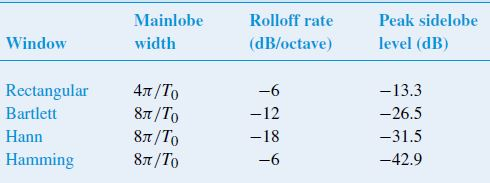
\includegraphics[scale=0.6]{Figures/DFT/other_windows_2}
\caption{Some continuous-time windows and their characteristics \cite{DSP_DimitrisManolakis}}
\label{fig:DFT:other_windows_2}
\end{figure}

\item Rectangular window has the narrower main lobe $\leftrightarrow$ highest resolution

	\begin{itemize}
	\item However, their side lobes are relatively high $\leftrightarrow$ poorest dynamic range
	\end{itemize}

\item Hamming window has a smoother transition in the time domain from $1 \rightarrow 0$

	\begin{itemize}
	\item Hence it has a wider mainlobe compared to the rectangular window $\leftrightarrow$ lower resolution
	
	\item But lower side lobes $\leftrightarrow$ higher dynamic range
	\end{itemize}

\item Chebyscheve window: we can control the side lobes height, and it has equal height side lobes

	\begin{itemize}
	\item The weaker the side lobes the more the transition is smooth
	
	\item Chebychev with -30 dB attenuation: narrower main lobe but high side lobes
	
	\item Chebychev with -70 db has quite the opposite compared to the -30 dB attenuation
	\end{itemize}

\item As a general rule: the more we push down the side lobes in the frequency domain (hence better dynamic range) $\leftrightarrow$ the main lobe will get higher (lower resolution)


\end{itemize}

\section{DTFT Spectrum Using Different Window Type}

\begin{itemize}

\item Example: $x[k] \, = \,\displaystyle\sum_{i \, = \, 1}^{i \, = \, 3} \text{Components}_i$

\begin{itemize}
\item $\text{Component 1 } = \, \text{cos} \left(\, \displaystyle\frac{\pi}{10} \, k \,\right) $
\item $ \text{Component 2 } = \,  \text{cos} \left(\, \displaystyle\frac{\pi}{8} \, k \, + \, \displaystyle\frac{\pi}{3} \right) $
\item $ \text{Component 3 } =  0.01 \, \text{cos} \left(\, \displaystyle\frac{4 \pi}{10} \, k \, - \,\displaystyle\frac{3 \pi }{5} \right) $ 
\end{itemize}


\item 2 criteria to be tested via the discrete signal $x[k]$: Resolution and Dynamic Range

 \begin{itemize}
 \item Resolution: the sum of 2 close signal $\leftrightarrow$ controlled by the width the main lobe
 
 \item Dynamic Range: displaying weak component $\leftrightarrow$ controlled by the height of the side lobes
 \end{itemize}

\newpage
\begin{figure}[ht]
\centering
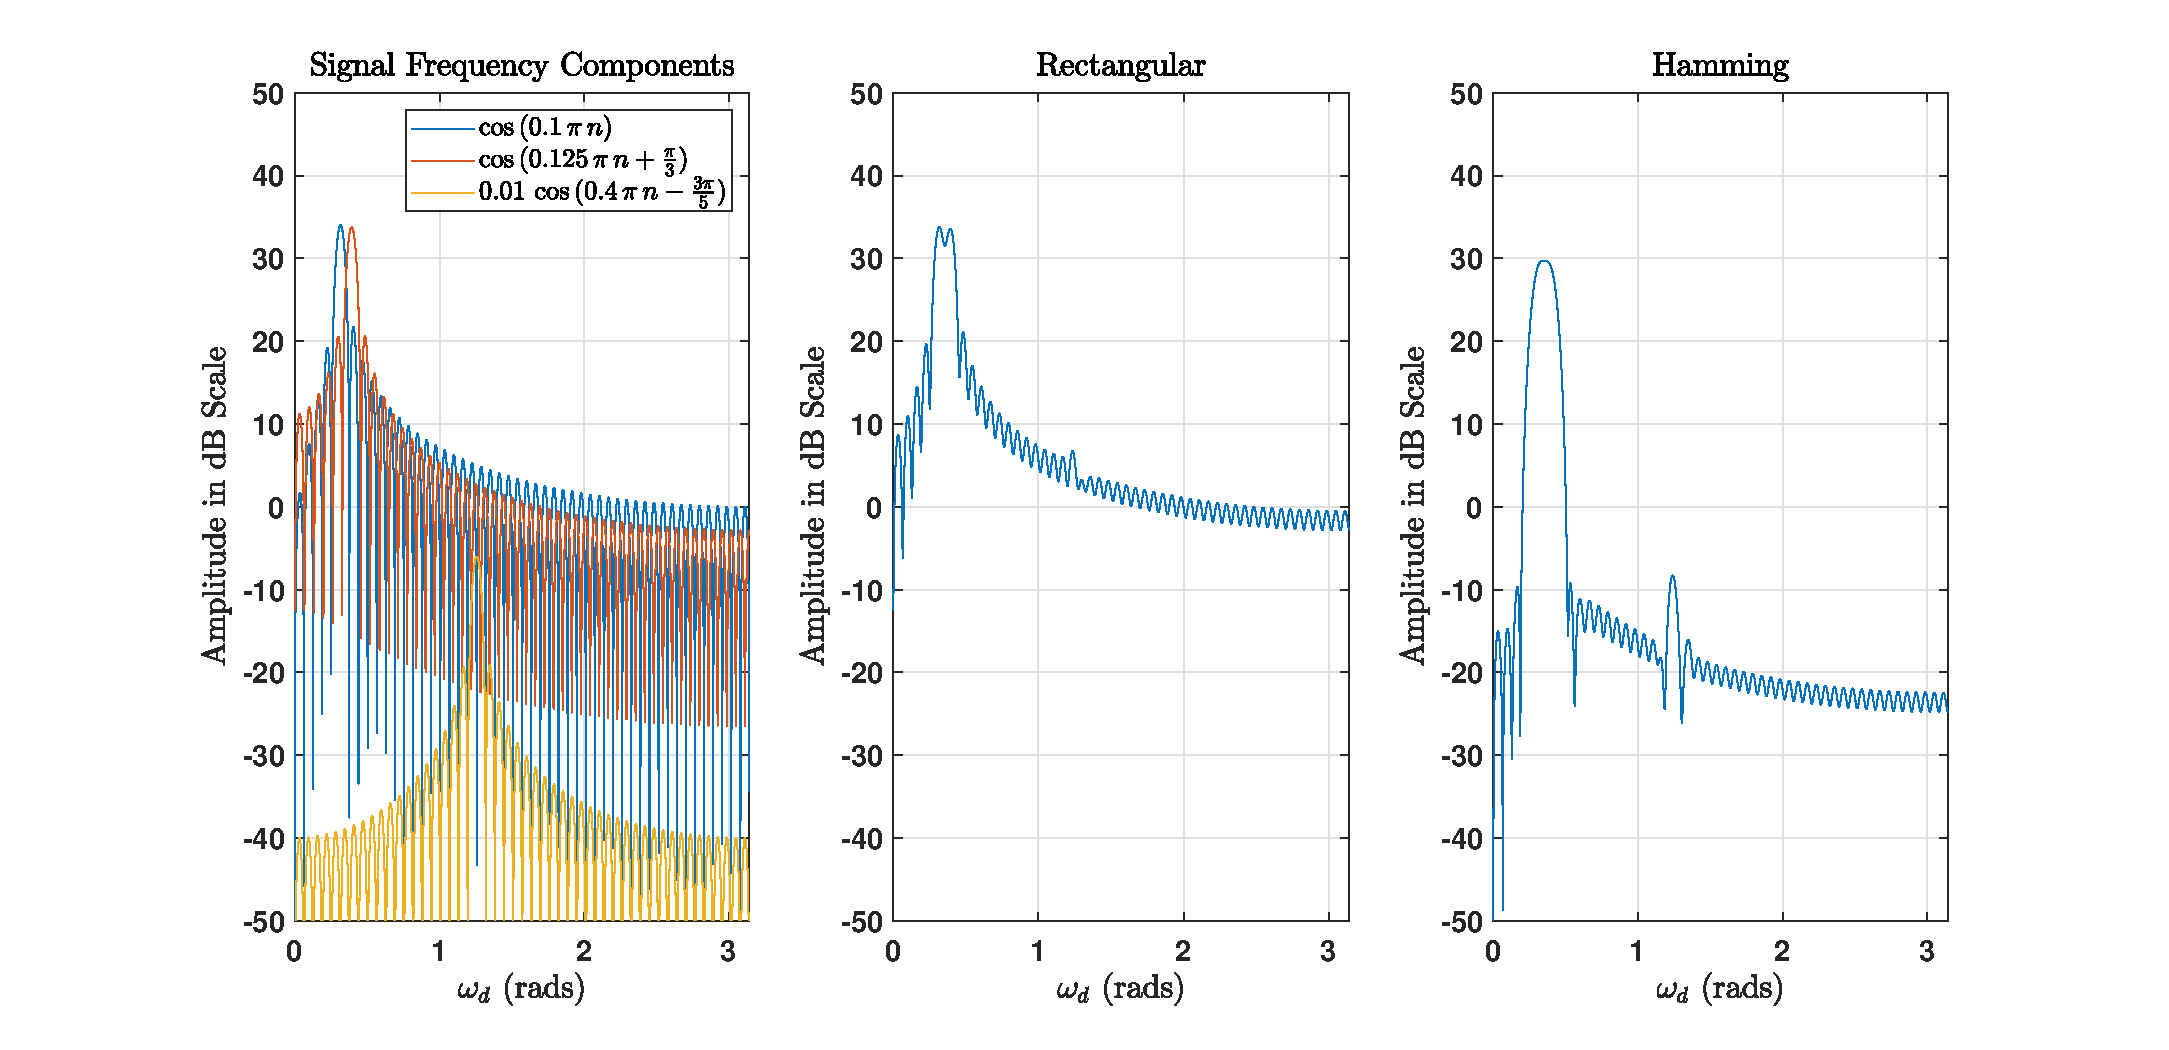
\includegraphics[scale=0.5]{Figures/DFT/sum_of_cos_rect_and_hamm.eps}
\caption{Rectangular and Hamming Window}
\label{fig:Papers:aliasing}
\end{figure}


\item In rectangular window:

	\begin{itemize}
	\item the 2 components  can be distinguished
	
	\item However the $\mathrm{3}^\mathrm{rd}$ components having a small amplitude has disappeared in the side lobes

	\begin{itemize}
	\item It barely  we can see it
	
	\item If we have some noisy data, it will completely		 gone
	\end{itemize}		

	\end{itemize}
	
\item In Hamming window:

\begin{itemize}
\item The 2 cos peaks has merged 

\item But the weak components is detected better then the rectangular window
\end{itemize}

\newpage

\begin{figure}[ht]
\centering
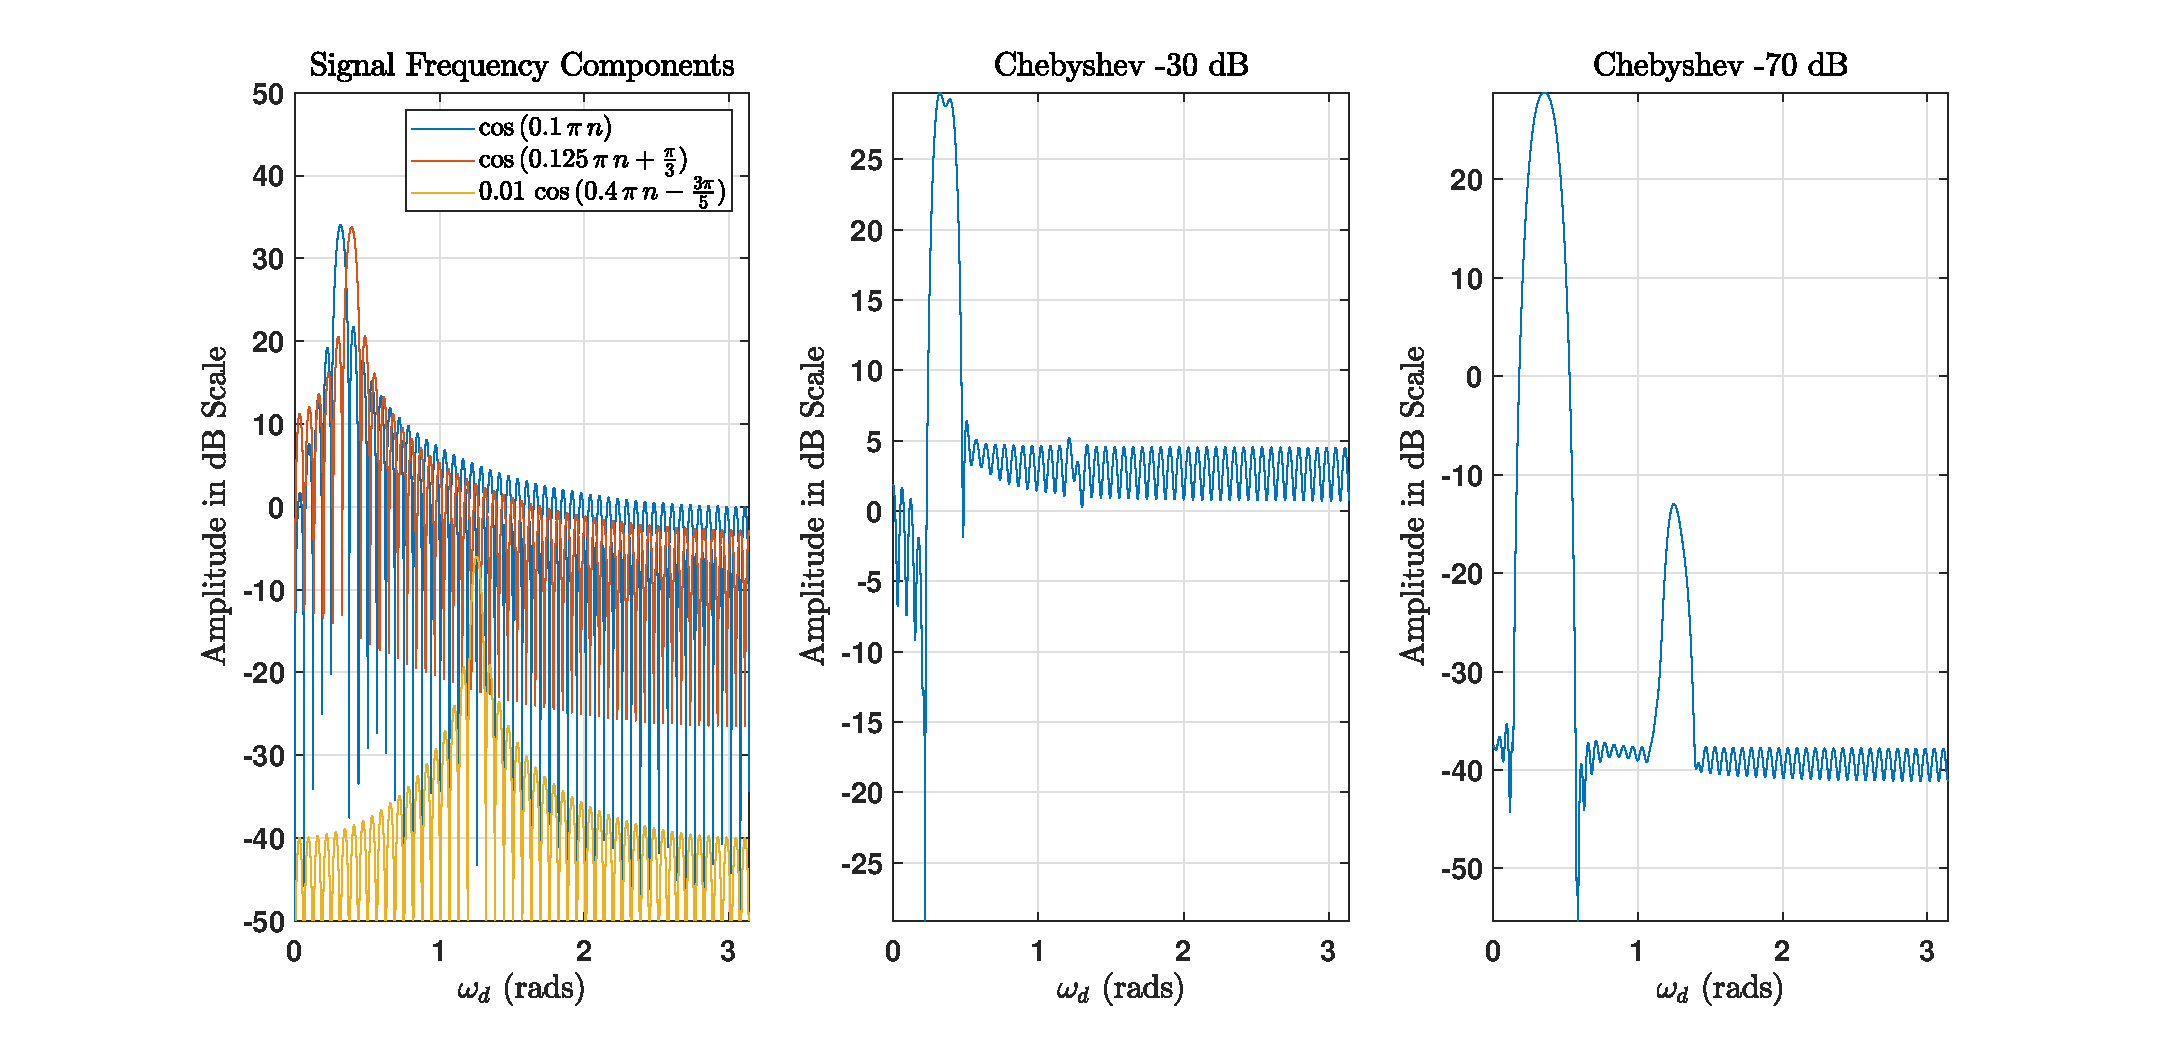
\includegraphics[scale=0.5]{Figures/DFT/sum_of_cos_chebyshev.eps}
\caption{Chebychves Window with -30 dB and -70 dB side lobes attenuation}
\label{fig:DFT:sum_of_cos_chebyshev}
\end{figure}

\item In -30 dB case:

	\begin{itemize}
	\item We can (although it is difficult) to see that we have 2 frequency components $\leftrightarrow$ good resolution
	
	\item However the weak component have vanished $\leftrightarrow$ poorer dynamic range
	\end{itemize}

\item In -70 dB case we have opposite results

	\begin{itemize}
	\item Since thee side lobes now are more attenuated, we can detect the weak component
	
	\item Of course in the price of poorer resolution as we can see, the 2 components are gone now
	\end{itemize}

\end{itemize}


\section{CTFT Analysis Using Different Window}

\begin{itemize}

\item We try to see now the effect of windows on CTFT spectrum for a damped cos signals given by:

\begin{equation*}
\begin{array}{rcl}
x(t) \, &=& \, e^{-0.1 \,t} \, \left[\, \text{cos}\left( \, 10 \, t \, \right) \, + \, \text{cos}\left( \, 12 \, t \, \right)  \,\right] \, u(t) \\ \\
X(\omega_c) \, &=& \, \displaystyle\frac{\, 0.1 \, + \, j \, \omega_c}{ \left( \, 0.1 \, + \, j \, \omega_c  \,  \right)^2    \, + \, 10^2} \, + \, \displaystyle\frac{0.1 \,+ \, j \, \omega_c}{ \left( \, 0.1 \, + \, j \, \omega_c  \,  \right)^2    \, + \, 12^2}
\end{array}
\end{equation*}


\begin{figure}[ht]
\centering
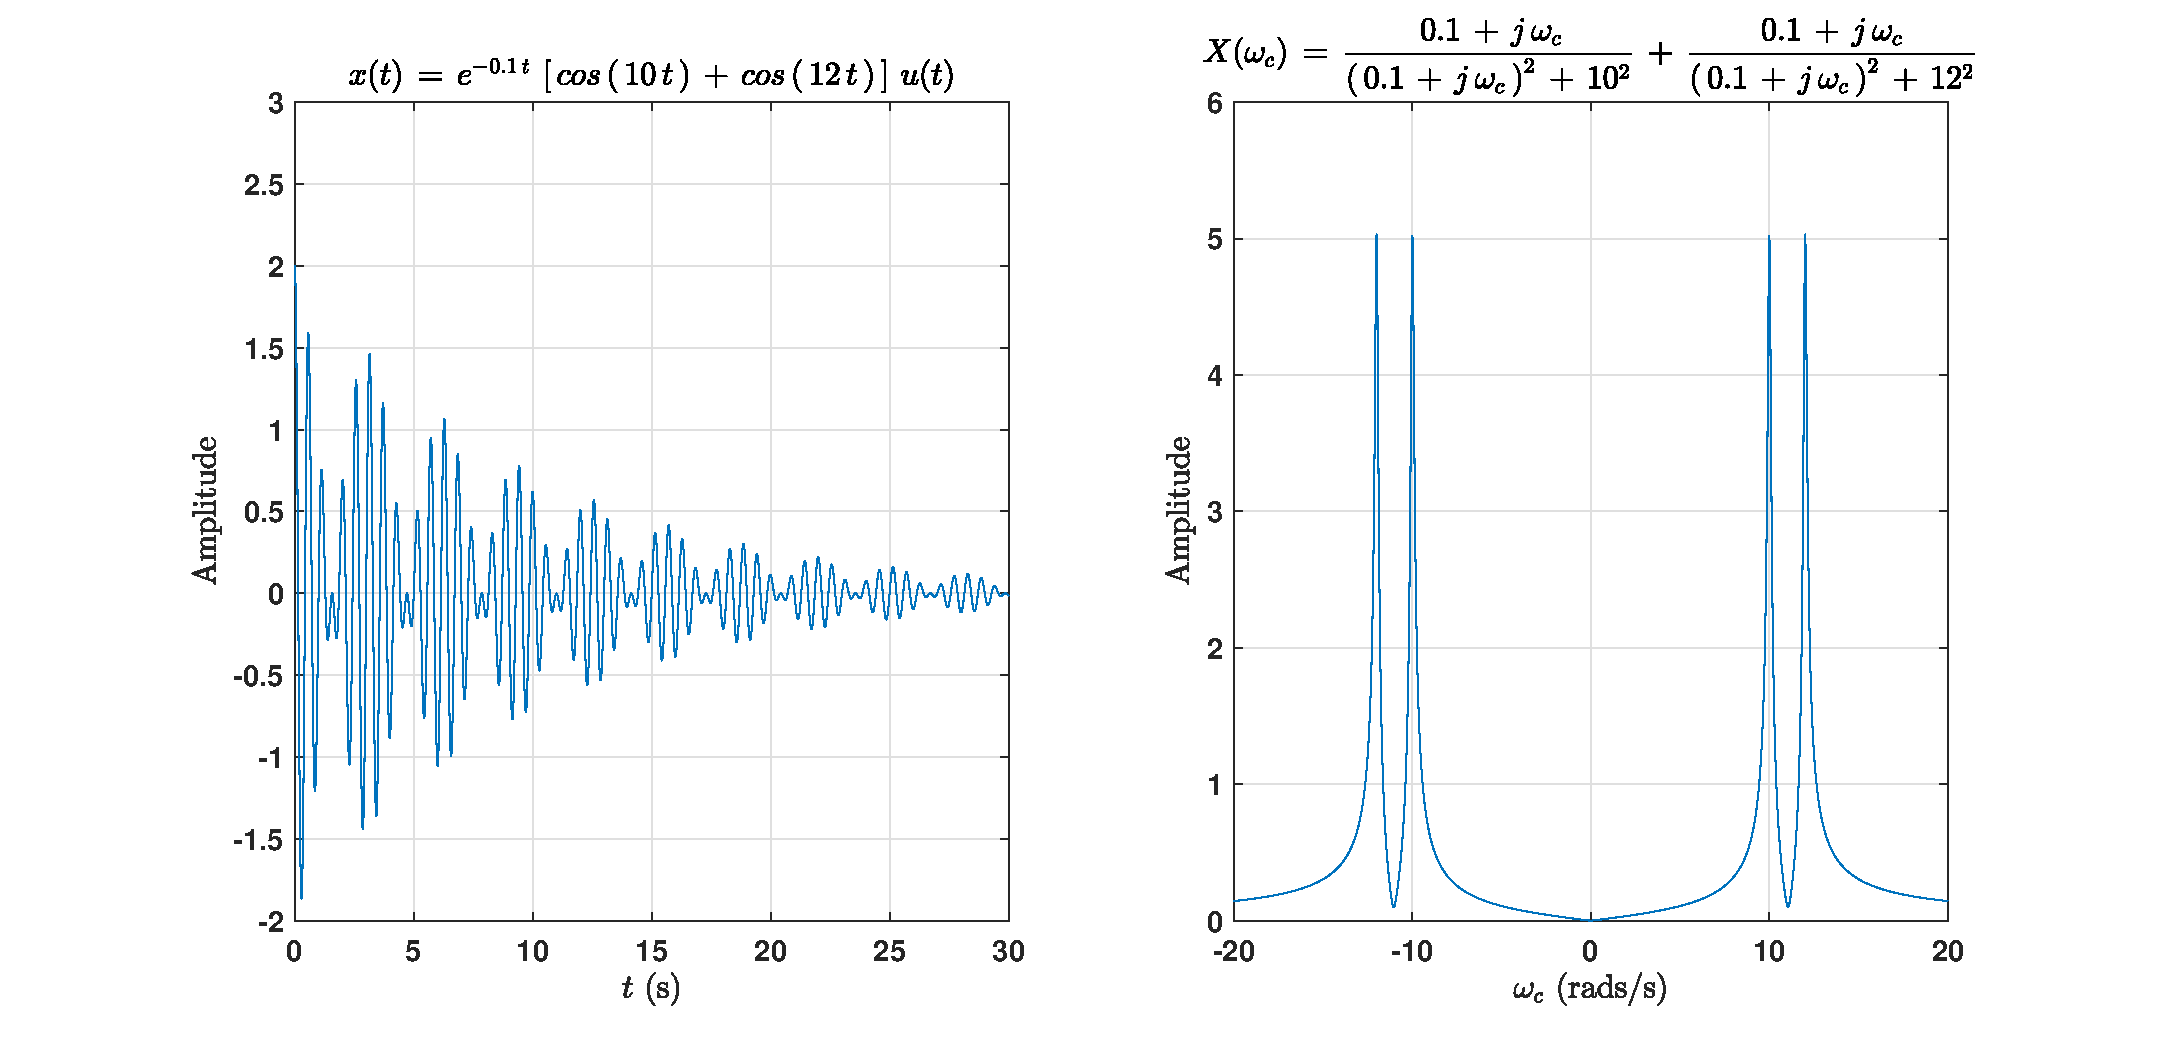
\includegraphics[scale=0.30]{Figures/DFT/damped_cosines_and_spectrum.eps}
\caption{$x(t)$ along with its Amplitude Spectrum}
\label{fig:DFT:damped_cosines_and_spectrum}
\end{figure}

\item $X(\omega_c)$ is not a bandlimited signal, so we need to choose a maximum frequency

	\begin{itemize}
	\item Since we can visualize that after 12 rad/s the spectrum roll off, we choose effective bandwidth of $B \, = \, 300$ rad/s $\rightarrow \, T_s \, = \, 0.01$ s
	\end{itemize}



\item We have 2 damped frequency components at 10 and 12 rad/s. Spectral Separation between these 2 components is $12 \, - \, 10 \,  = \, 2 $ rad/s 

\item Recall that the width of the main lobe need to be smaller than the spectral separation

\item We choose to see details at 2 resolution using rectangular window:

	\begin{enumerate}
	\item $\displaystyle\frac{2 \pi}{5} \, \approx \, 1.2566 <<  2$ rad/s
	
		\begin{itemize}
		\item $\displaystyle\frac{4 \pi}{\text{Signal Duration}} \, = \,   \displaystyle\frac{4 \pi}{T_s \, N} \leq \, \displaystyle\frac{2 \pi}{5} \rightarrow \, N \, \geq \, 1000 $ samples
		\end{itemize}
		
	\item We increase resolution times 5: $\displaystyle\frac{2 \pi}{25} \, \approx \, 0.2513$
	
	\begin{itemize}
		\item $\displaystyle\frac{4 \pi}{\text{Signal Duration}} \, = \,   \displaystyle\frac{4 \pi}{T_s \, N} \leq \, \displaystyle\frac{2 \pi}{25} \rightarrow \, N \, \geq \, 5000 $ samples
		\end{itemize}

	\end{enumerate}
	
\begin{figure}[ht]
\centering
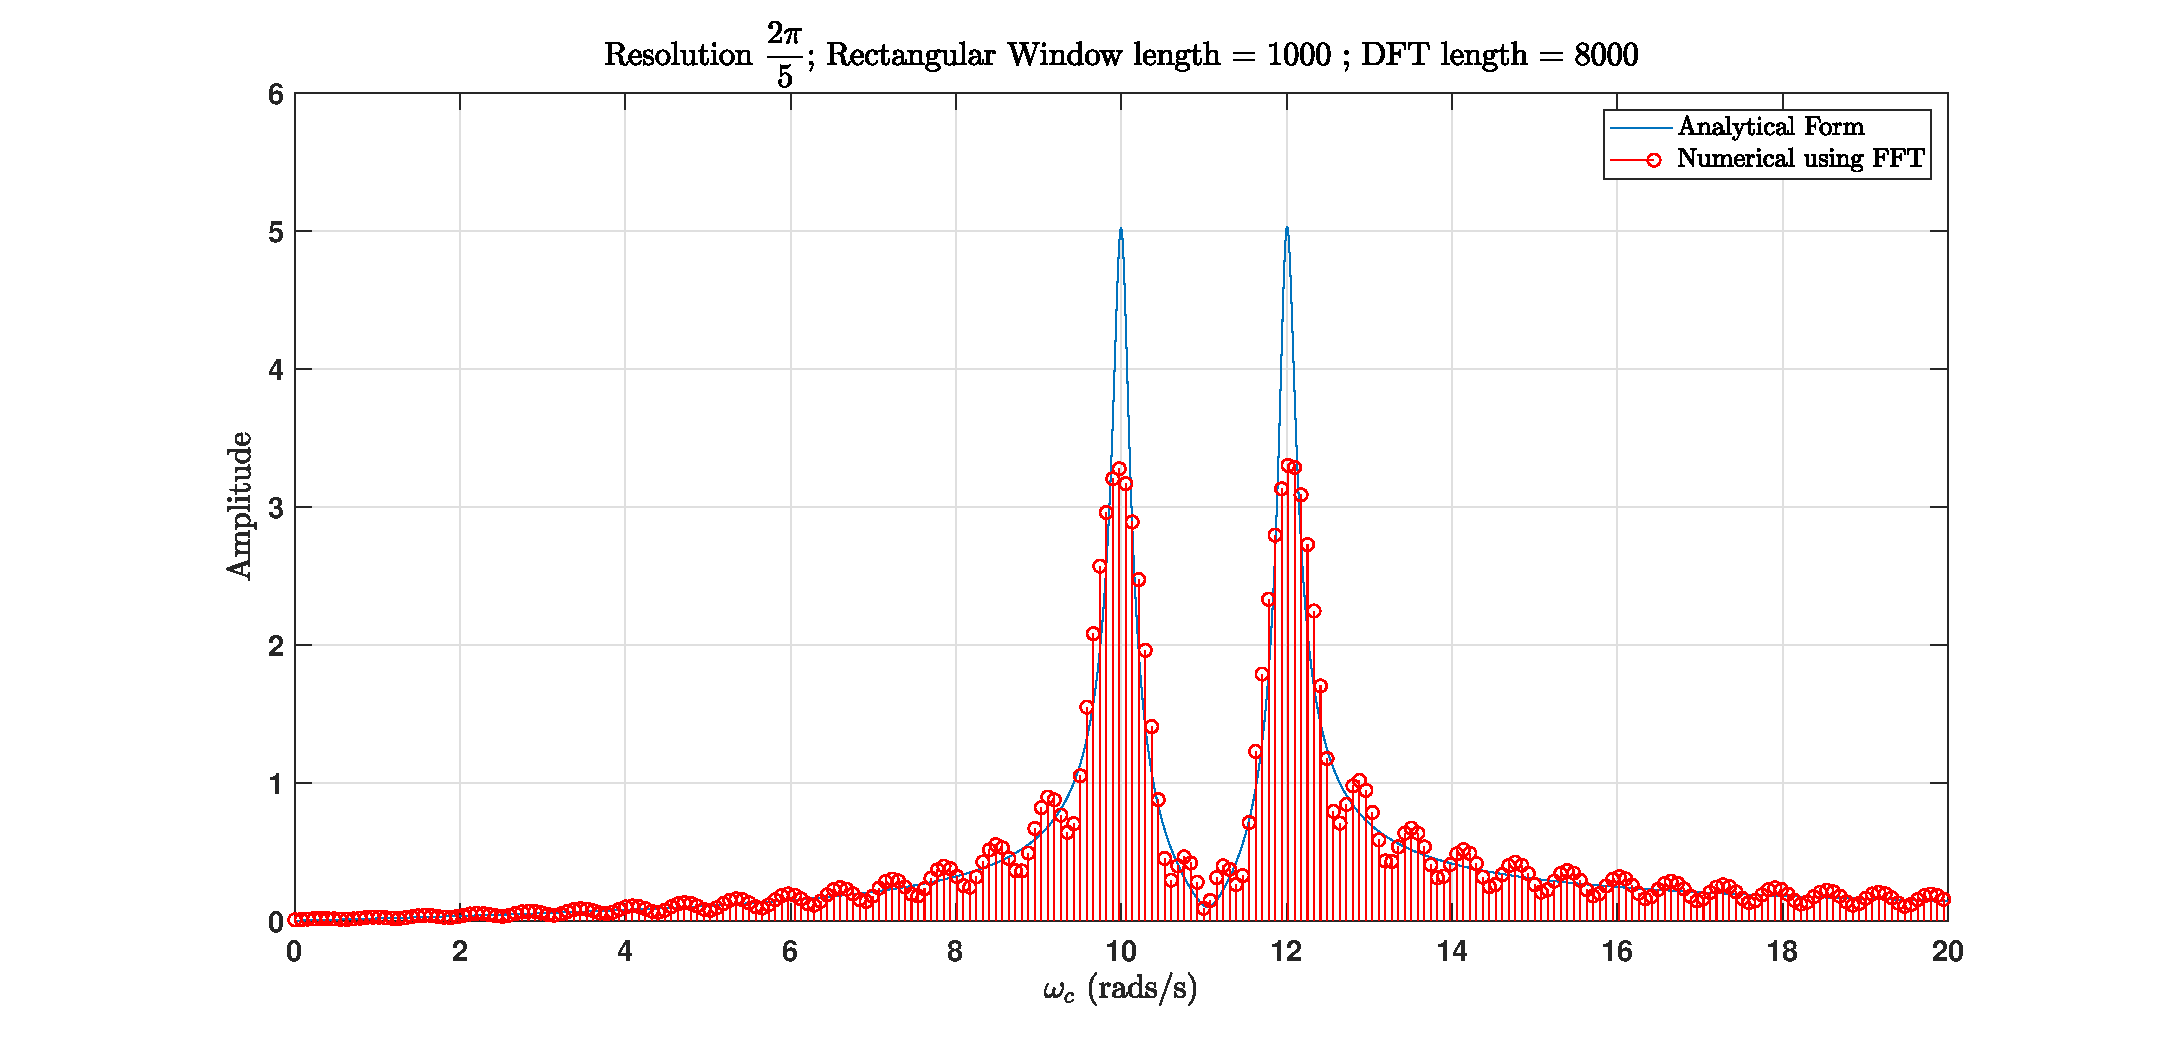
\includegraphics[scale=0.30]{Figures/DFT/spectrum_rect_window_length_1000.eps}
\label{fig:DFT:spectrum_rect_window_length_1000}
\end{figure}

\begin{itemize}

\item DFT Values are distorted

\item Some ripples at the tails

\end{itemize}


\item Increasing resolution 5 times from $\displaystyle\frac{2 \pi}{5} \rightarrow \displaystyle\frac{2 \pi}{25}$ (narrower main lobe)


	\begin{itemize}
	\item Better DFT Values and  No ripples at the tails
	\end{itemize}


\begin{figure}[ht]
\centering
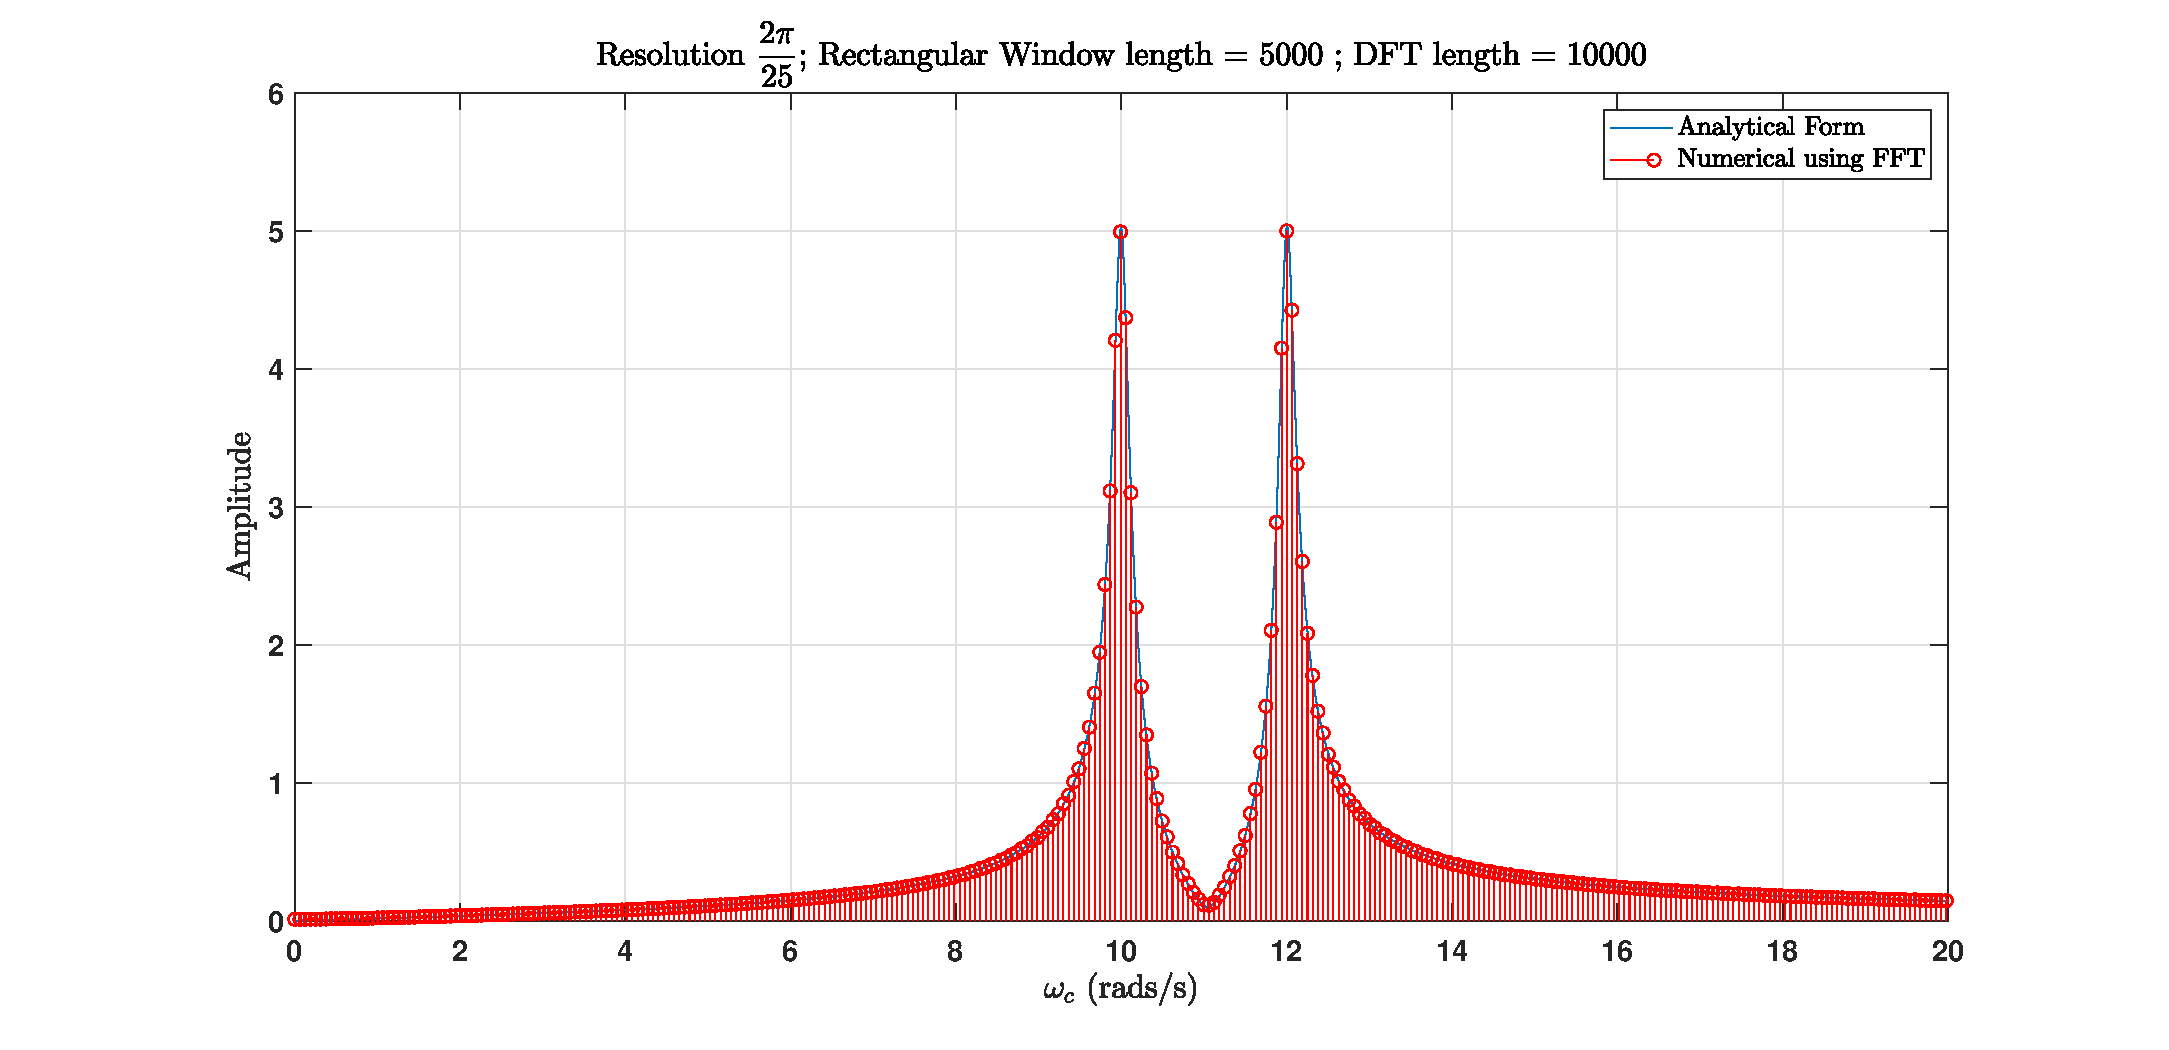
\includegraphics[scale=0.26]{Figures/DFT/spectrum_rect_window_length_5000.eps}
\label{fig:DFT:spectrum_rect_window_length_5000}
\end{figure}

\item Trying Different type of Windows: Hamming window for example, with the best observed resolution which is $  \displaystyle\frac{2 \pi}{25}$

\item Hamming Length:

	\begin{itemize}
	\item $\displaystyle\frac{8 \pi}{\text{Signal Duration}} \, = \,   \displaystyle\frac{8 \pi}{T_s \, N} \leq \, \displaystyle\frac{2 \pi}{5} \rightarrow \, N \, \geq \, 10^4 $ samples
	
	\item Rectangular window length was 5000 samples for a resolution  of $  \displaystyle\frac{2 \pi}{25}$
	
	\item Hamming need 2 times more samples then rectangular to observe same level of details
	\end{itemize}


\begin{figure}[ht]
\centering
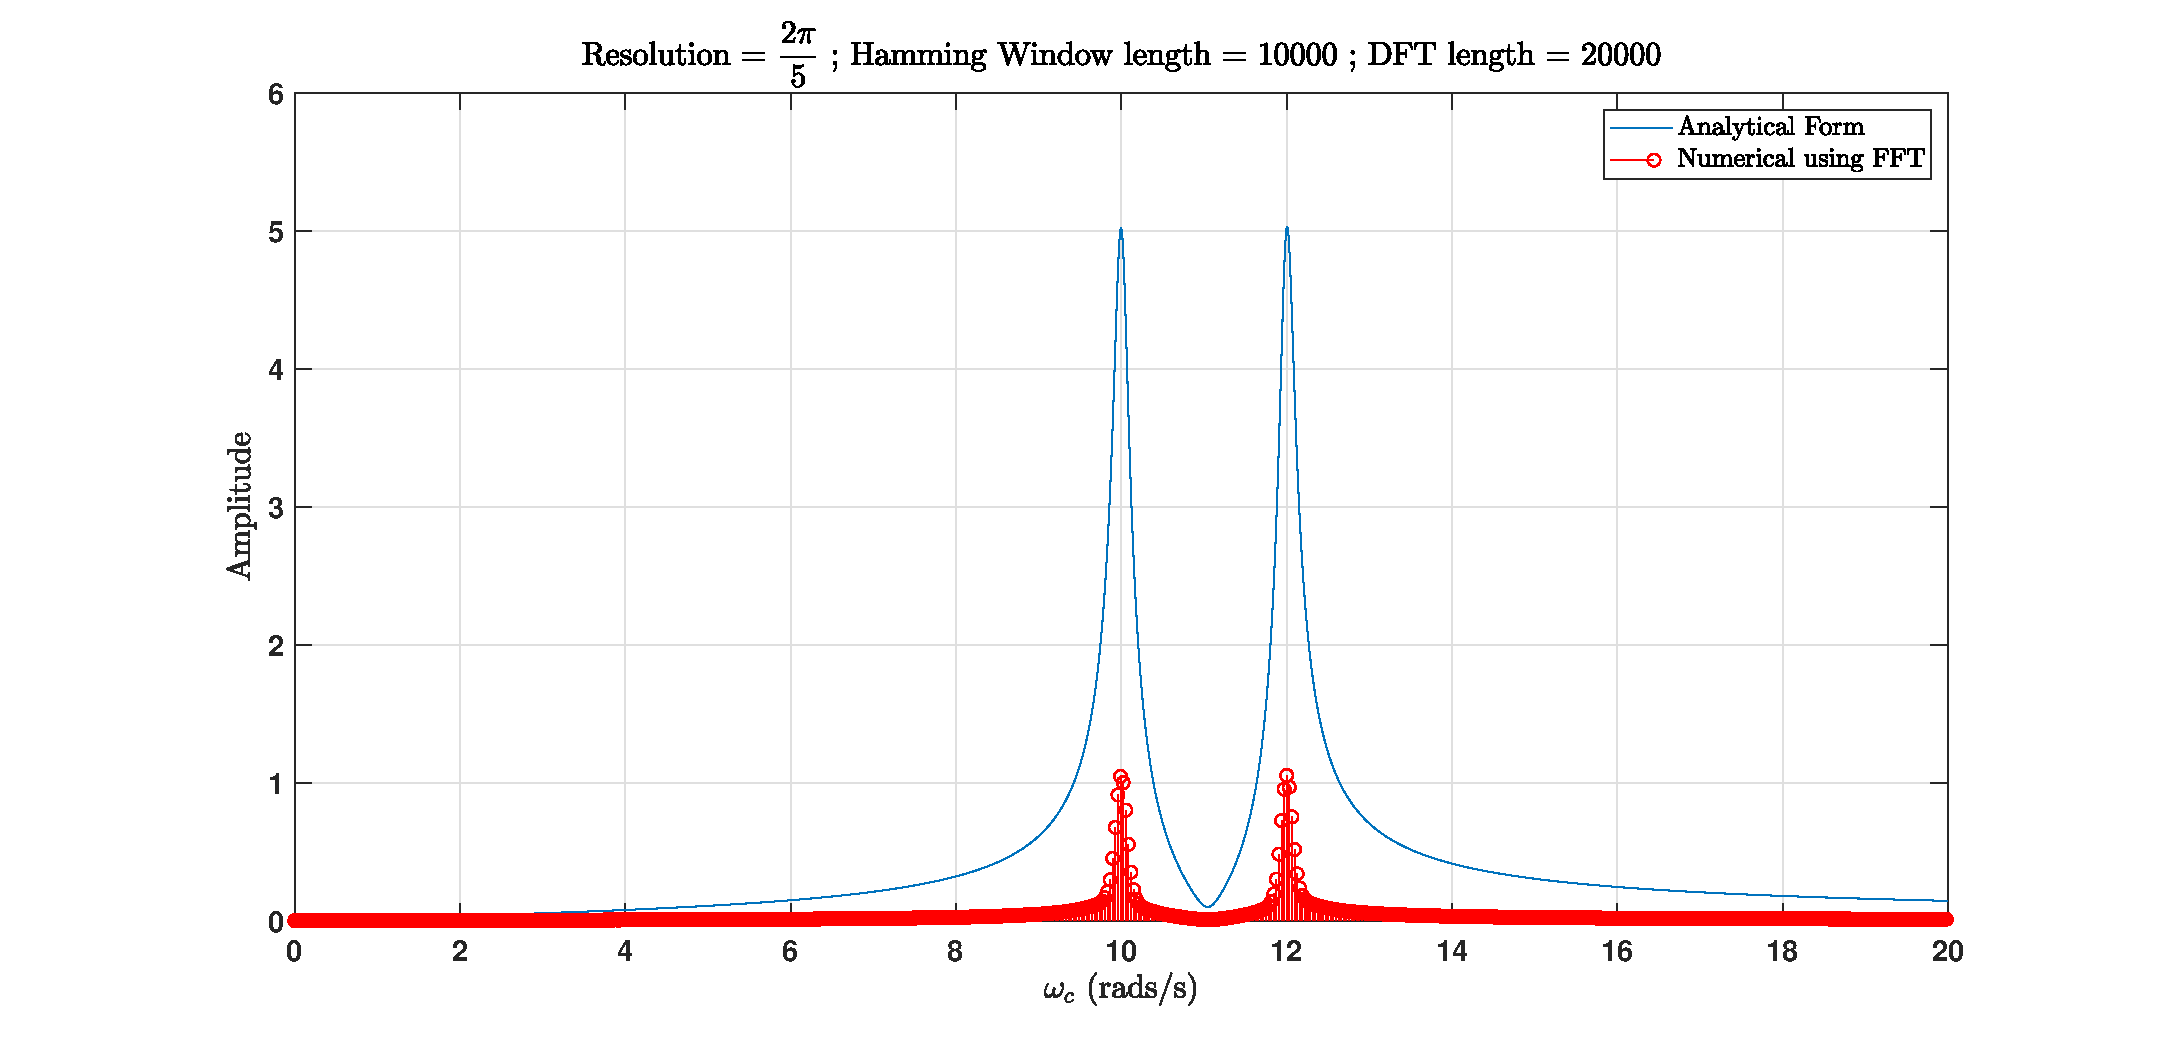
\includegraphics[scale=0.26]{Figures/DFT/spectrum_hamming_window_length_10_pow_4.eps}
\label{fig:DFT:spectrum_hamming_window_length_10_pow_4}
\end{figure}

\item DFT amplitude values are very distorted

\item Hamming is attenuating signal energy when we are windowing 

\begin{figure}[ht]
\centering
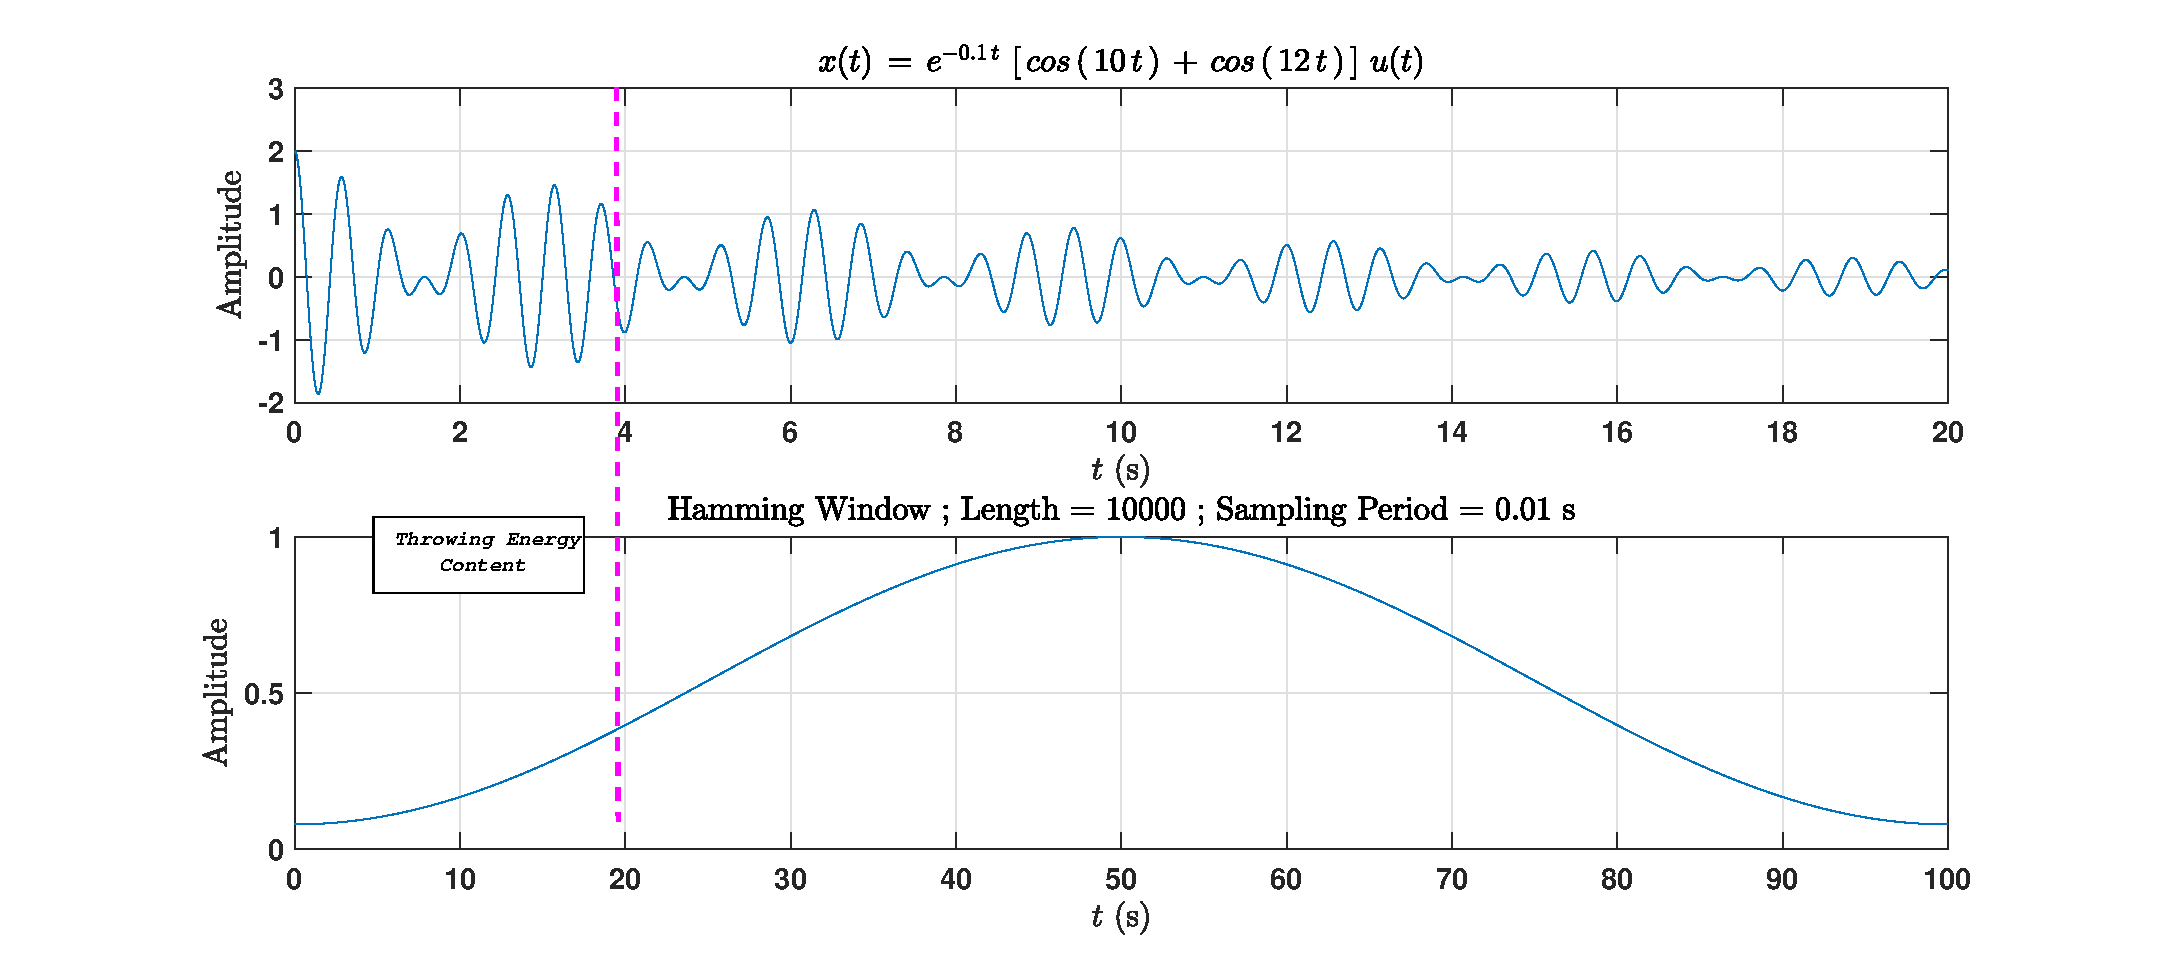
\includegraphics[scale=0.30]{Figures/DFT/hamm_signal_plot_time_domain_2.eps}
\label{fig:DFT:hamm_signal_plot_time_domain_2}
\end{figure}	
	

\end{itemize}


%***************************************
%***************************************
%***************************************


\chapter{Complex Number and Low Pass Simulation}

\underline{References:} chapter 5 in \cite{book_SDR_BobStewart} and chapter 4 in \cite{book_comm_system_sim_Tranter}

\section{Review of Basics}

\begin{itemize}

\item Advantage of complex notation: easier to work with multiplication of complex exponential rather then the multiplication of 2 cos

    \begin{itemize}
        \item $e^{j \, A} \, e^{j \, B} \, = \, e^{j \, (\, A \, + \, B \, )}$
        
        \item $\cos(A) \, \cos(B) \, = \, \displaystyle\frac{1}{2} \, \left[\, \cos( \, A \, + \, B \, ) \, + \, \cos( \, A \, - \, B \, )    \, \right]$
    \end{itemize}

\item Signal processing work with voltages to process real world quantities

\begin{itemize}
    \item When the antenna see the change in the EM field, it induces voltages
    
    \item Microphone pick up sound waves from small changes in sound pressure to produce voltage
\end{itemize}


\end{itemize}


\newpage
\section{Quadrature Representation}


\subsection{Case Usage}

IQ signals are used in many places. In communication applications:

\begin{itemize}
    \item Used in Tx side to \tbi{unify many modulation scheme} (as shown in \autoref{fig:Sampling:qudrature_impelmentation})
    
    \begin{itemize}
        \item Instead of using different circuitry for each modulation type, we can change the IQ values to obtain various modulation type
    \end{itemize}
    

\item Used in Rx for demodulation as shown in \autoref{fig:Sampling:I_Q_system}

\begin{figure}[ht]
\centering
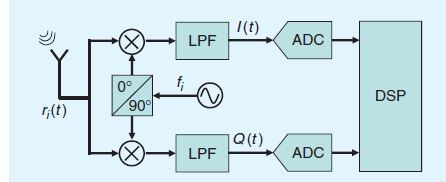
\includegraphics[width = 0.7\textwidth]{Figures/Sampling/I_Q_system}
\caption{A block diagram of a typical I-Q demodulator \cite{Sub_Nyquist_sampling}}
\label{fig:Sampling:I_Q_system}
\end{figure}


    
\end{itemize}

\todo{Case Usage}

\textit{Try to simulate these idea in practical application}



\subsection{Formula}


\begin{equation}
\begin{array}{lll}
x_{\text{band-pass}}(t) \, &=&\, \text{Amp}(t) \, \times \, \text{cos}\left(\, 2 \pi \, f_{\text{center}} \, t \, + \, \text{phase}(t) \,\right)\\ \\
        &=& \, x_{\text{in-phase}}(t) \, \text{cos}\left(\, 2 \pi \, f_{\text{center}} \, t \,\right) + \, x_{\text{quadrature}}(t) \, \text{sin}\left(\, 2 \pi \, f_{\text{center}} \, t \,\right) 
\end{array}
\label{Eq:Sampling:based_band_general_form_time_domain}
\end{equation}

where $\begin{cases}
x_{\text{Eq-Baseband}}(t) \, = \, \text{Amp}(t)\,\times \, \text{exp}\left[\, j \,\times \, \text{phase}(t) \,\right] \\ \\
\text{Amp}(t) \, = \, \sqrt{ x_{\text{in-phase}}^2(t) \, + \, x_{\text{quadrature}}^2(t)} \\ \\
\text{phase}(t) \,  = \, \text{tan}^{-1}\left[\, \displaystyle\frac{ x_{\text{quadrature}}(t)}{x_{\text{in-phase}}(t)} \,\right] 
\end{cases}$



\newpage

\subsection{Summary for IQ Representation}

\begin{figure}[ht]
\centering
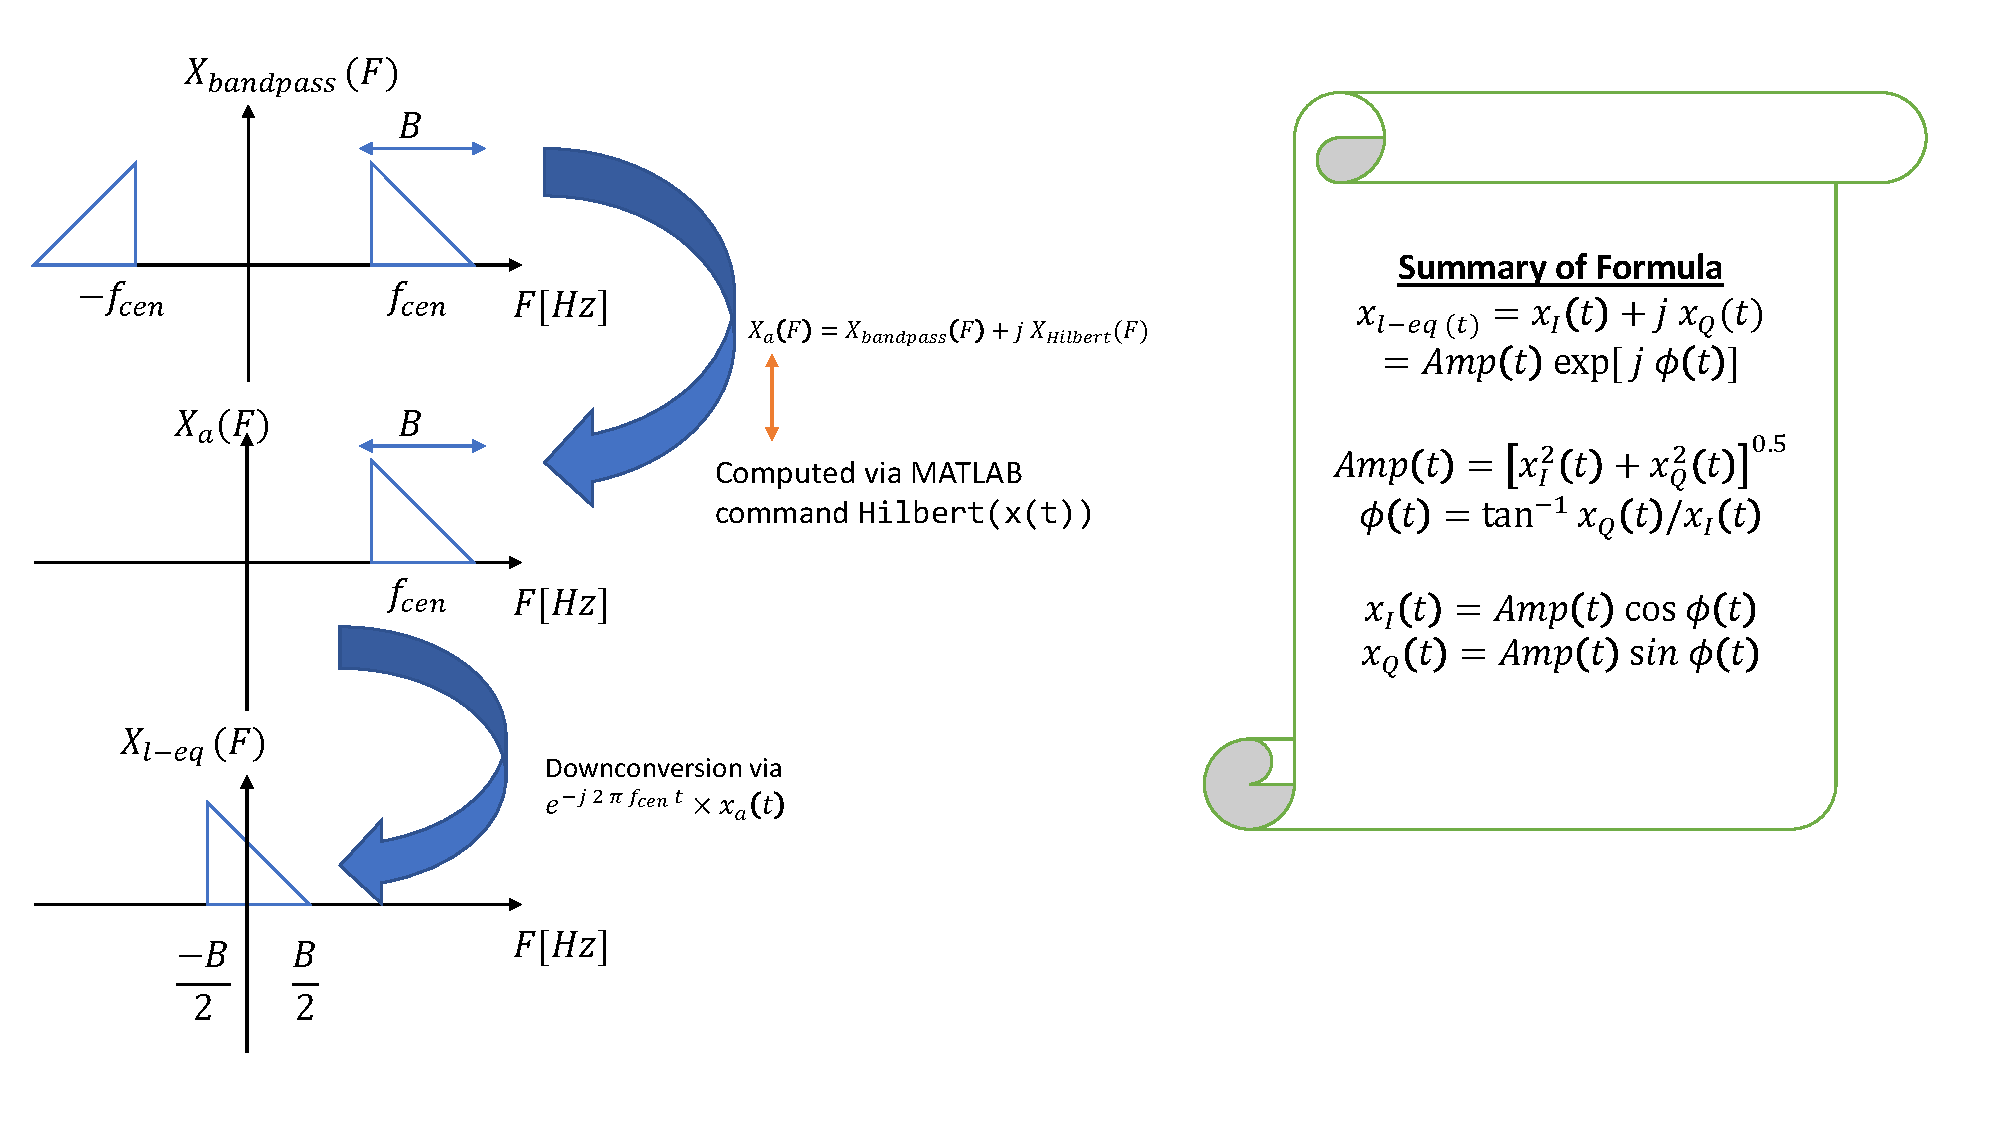
\includegraphics[width = 0.7\textwidth, frame]{Figures/Sampling/summary_IQ}
\caption{Summary for IQ Representation}
\label{fig:Sampling:summary_IQ}
\end{figure}

\subsection{Analog Generation of IQ Signals}

\begin{figure}[ht]
\centering
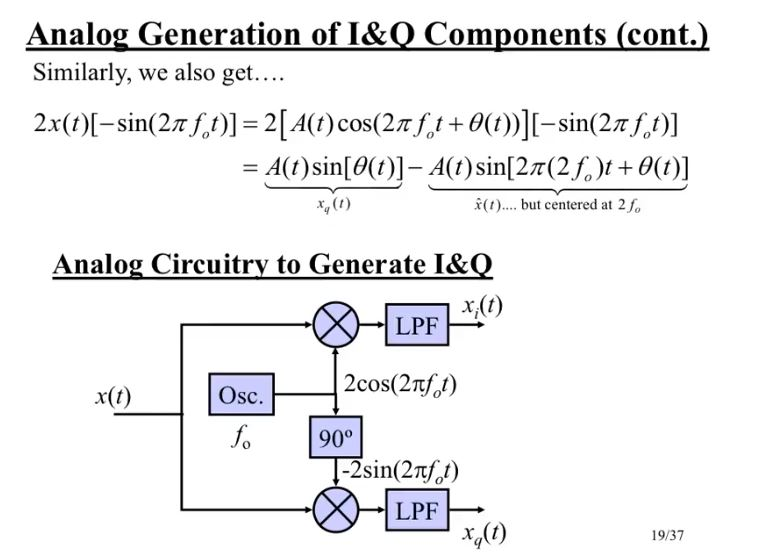
\includegraphics[width = 0.7\textwidth, frame]{Figures/Sampling/qudrature_impelmentation}
\caption{IQ generation and implementation using analog devices}
\label{fig:Sampling:qudrature_impelmentation}
\end{figure}


\newpage
\section{Examples}

\begin{itemize}
    
    \item \todo{FFT leakage}
    
    Ex 5.1 page 175 in \cite{book_SDR_BobStewart}: contains nice explanation about leakage and bins resolution
  
 \end{itemize}
 
 
 \subsection{AM Signals}
 
Let the signal $x(t)$ given by:
 
\begin{equation}
    x(t) \, = \, 
\end{equation} 
 
 \subsection{FM Signals}
 
 
 First we recall the FM signal model:
 
 \begin{equation}
    x_{\text{FM}}(t) \, = \, A_c \, \cos{ \left( \,  2 \pi f_c \, t \, + \, 2 \pi K_{\text{FM}} \, \times \, \displaystyle\int_{- \infty}^t  m(t)\, dt  \,\right)}
\label{Eq:FM:equation_tx}
\end{equation}

In case of FM, $\Phi(t) \, = \, \displaystyle\int_{- \infty}^t  m(t)\, dt$, hence the IQ components are:

\begin{eqnarray}
 I_{\text{FM}}(t) \, &=& \,  A_c \, \cos{ \left(  \, 2 \pi K_{\text{FM}}  \, \displaystyle\int_{- \infty}^t  m(t)\, dt  \,\right)} \\ \\
  Q_{\text{FM}}(t) \, &=& \,  A_c \, \sin{ \left(  \, 2 \pi K_{\text{FM}}  \, \displaystyle\int_{- \infty}^t  m(t)\, dt  \,\right)}
\end{eqnarray}
 
 
 \newpage
\subsection{Design Criteria: Carrier Synchronization and Phase locked Loop}

\underline{Source:} 

\begin{itemize}

\item Begin with a refresher about AM-DSB-SC, section 5 page 182 \cite{book_SDR_BobStewart}

\item Phase Error See section 5.3.3 in \cite{book_SDR_BobStewart} :
    
        \begin{itemize}
            \item In demodulation, the oscillator may not be synchronized with the carrier $\leftrightarrow$ we have some phase $\theta$
            
            \item For a base band message $g(t) \, = \,A \, \cos (2 \pi f_b \, t)$, the demodulation will give: $ \hat{m}(t) \, = \,  \displaystyle\frac{A}{2} \, g(t) \, \cos \, ( \, \theta \, )$
            
            \item for $\theta \, = \, \pm \displaystyle\frac{\pi}{2}$, $\hat{m}(t) \, = \, 0$, that's why we need carrier synchronization and phase locking at the Rx side
            
            
        \end{itemize}
 
\item QAM: a method to transmit 2 data streams on the same carrier, but with a separate offset 

This a more bandwidth efficient scheme.

If we want to compare it to AM-DSB-SC: we need 2 times the bandwidth in AM-DSB-SC for transmission, but in QAM we only need $f_b$.

\begin{itemize}
    \item QAM Tx Side
    
\begin{figure}[ht]
\centering
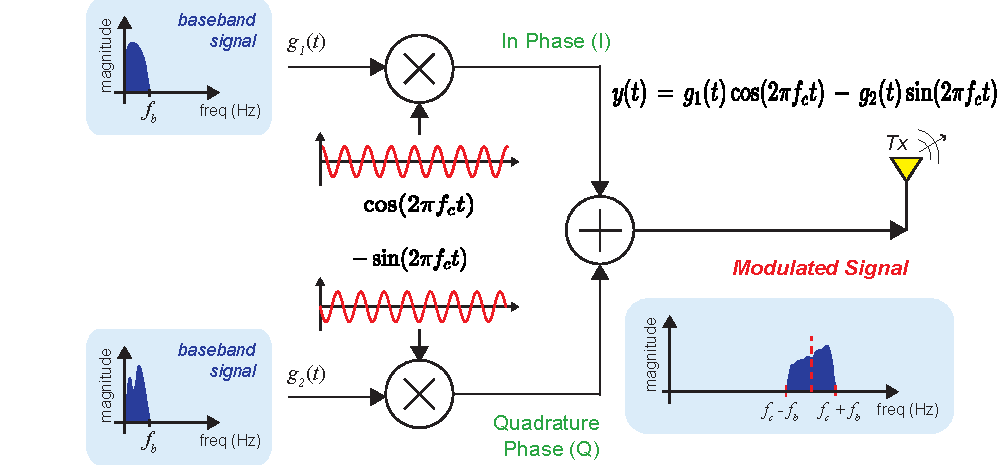
\includegraphics[scale=0.7]{Figures/Complex_Low_Pass/QAM_Tx}
\caption{QAM Tx Side}
\label{fig:Complex_Low_Pass:QAM_Tx}
\end{figure}    
    
    
    \item QAM Rx Side
    
\begin{figure}[ht]
\centering
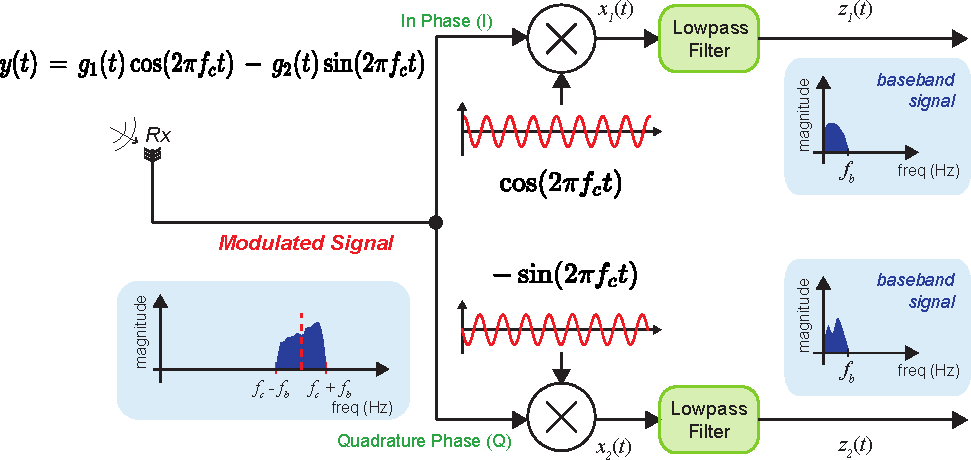
\includegraphics[scale=0.7]{Figures/Complex_Low_Pass/QAM_Rx}
\caption{QAM Rx Side}
\label{fig:Complex_Low_Pass:QAM_Rx}
\end{figure}    
    
    
\end{itemize}

\newpage
\item Using Complex Notation: the key in complex notation is to remember \autoref{Eq:Phasor_Notation}

\begin{equation}
\cos (2 \pi f_c t) \, = \, \text{Re}(e^{j 2 \pi f_c t})    
\label{Eq:Phasor_Notation}
\end{equation}
  
  
\newpage    
In \autoref{fig:Complex_Low_Pass:QAM_Tx_Rx_Complex}, we have the equivalent Tx-Rx QAM scheme using complex notation

\begin{figure}[ht]
\centering
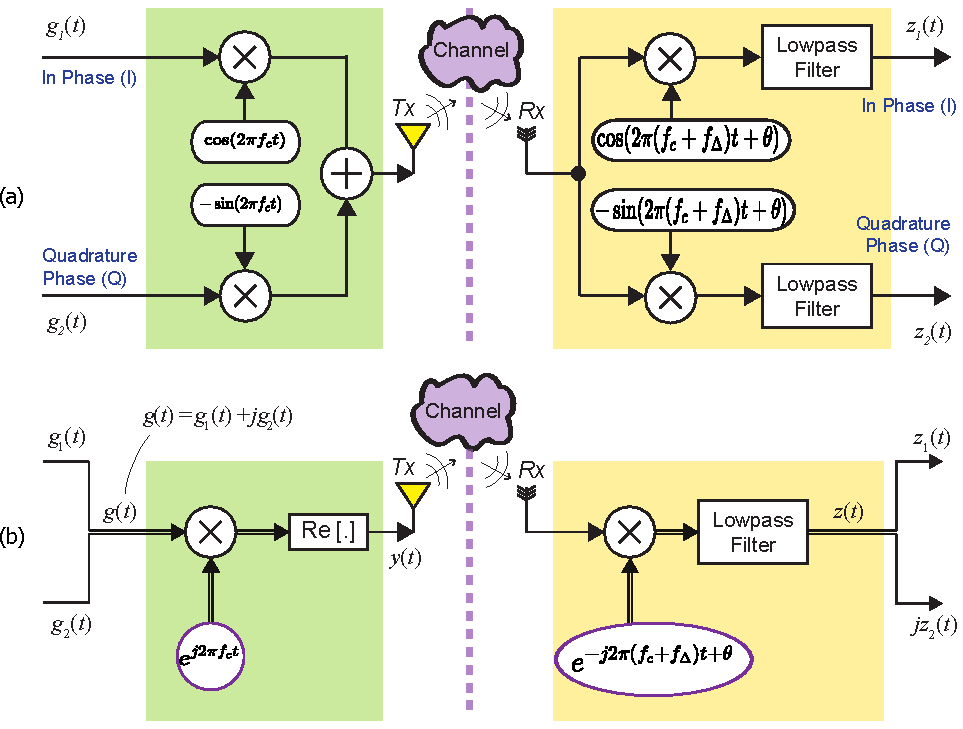
\includegraphics[scale=0.7]{Figures/Complex_Low_Pass/QAM_Tx_Rx_Complex}
\caption{QAM Tx-Rx Using Complex Notation}
\label{fig:Complex_Low_Pass:QAM_Tx_Rx_Complex}
\end{figure}    
    

    
\end{itemize}


%***************************************
%***************************************
%***************************************


\chapter{Power Spectral Density}

\section{Introduction}

Spectral Analysis: characterize power distribution over frequency using finite amount of time series data (chapter 1 in \cite{book_Spectral_Analysis_Stoica}).\\

The PSD concept is important to use in communication signals, where they are random in nature, and hence they have infinite power. To analyze such signals, PSD concept is used (see section 1.2.4 \cite{books_digital_comm_fundamentals_Sklar})

For a nice introduction and reviewing concept:\\

\begin{itemize}
    \item See chapter 1 (mainly 1.3) in \cite{book_Spectral_Analysis_Stoica}

\end{itemize}

\section{Pwelsh Method}

We start by simple simulation of a sin function:

\begin{equation}
    x(t) \, = \, A \, \sin{2 \pi f \, t} \quad \text{where } f \, = \, 500 \text{Hz and } A \, = \, \sqrt{2}
\end{equation}

We take $F_s \, = \, 4$KHz and number of point to generate 1024.\\

Analytically, power of $x(t) \, = \, \displaystyle\frac{A^2}{2} \, = 1$ Watt $\rightarrow 10 \log_{10} (\, 1\, ) \, = \, 0$ dBW/Hz.

\subsection{Reminder of Power Notion}

See section 2.5 in \cite{books_principle_of_system_Ziemer}.

\begin{itemize}
    \item PSD gives power per frequency components $\leftrightarrow$ Watt/Hz
    
    \item The \tbi{total power} or \tbi{average power} is the sum of the PSD (integration to be precise)
    
    \item For sin and cos signals:
    
    \begin{itemize}
        \item PSD is $\displaystyle\frac{A^2}{4}$
        
        \item Average power $= \displaystyle\frac{A^2}{4} \, + \, \displaystyle\frac{A^2}{4} \, = \, \displaystyle\frac{A^2}{2}$
    \end{itemize}
    
\end{itemize}

\subsection{Matlab Simulation}

In Maltab, we can use the \verb|pwelsh| function to compute the average power where:

\verb|[pxx,f]= pwelch(signal,window,n_overlapp,nfft,fs);| where:

\begin{itemize}

    \item \verb|nfft = Nb_samples = | 1024
    
    \item \verb|window = rectwin(nfft);|
\end{itemize}

\autoref{fig:PSD_Com:Demo_PSD_Sin} show the results of the simulation.

\begin{figure}[ht]
\centering
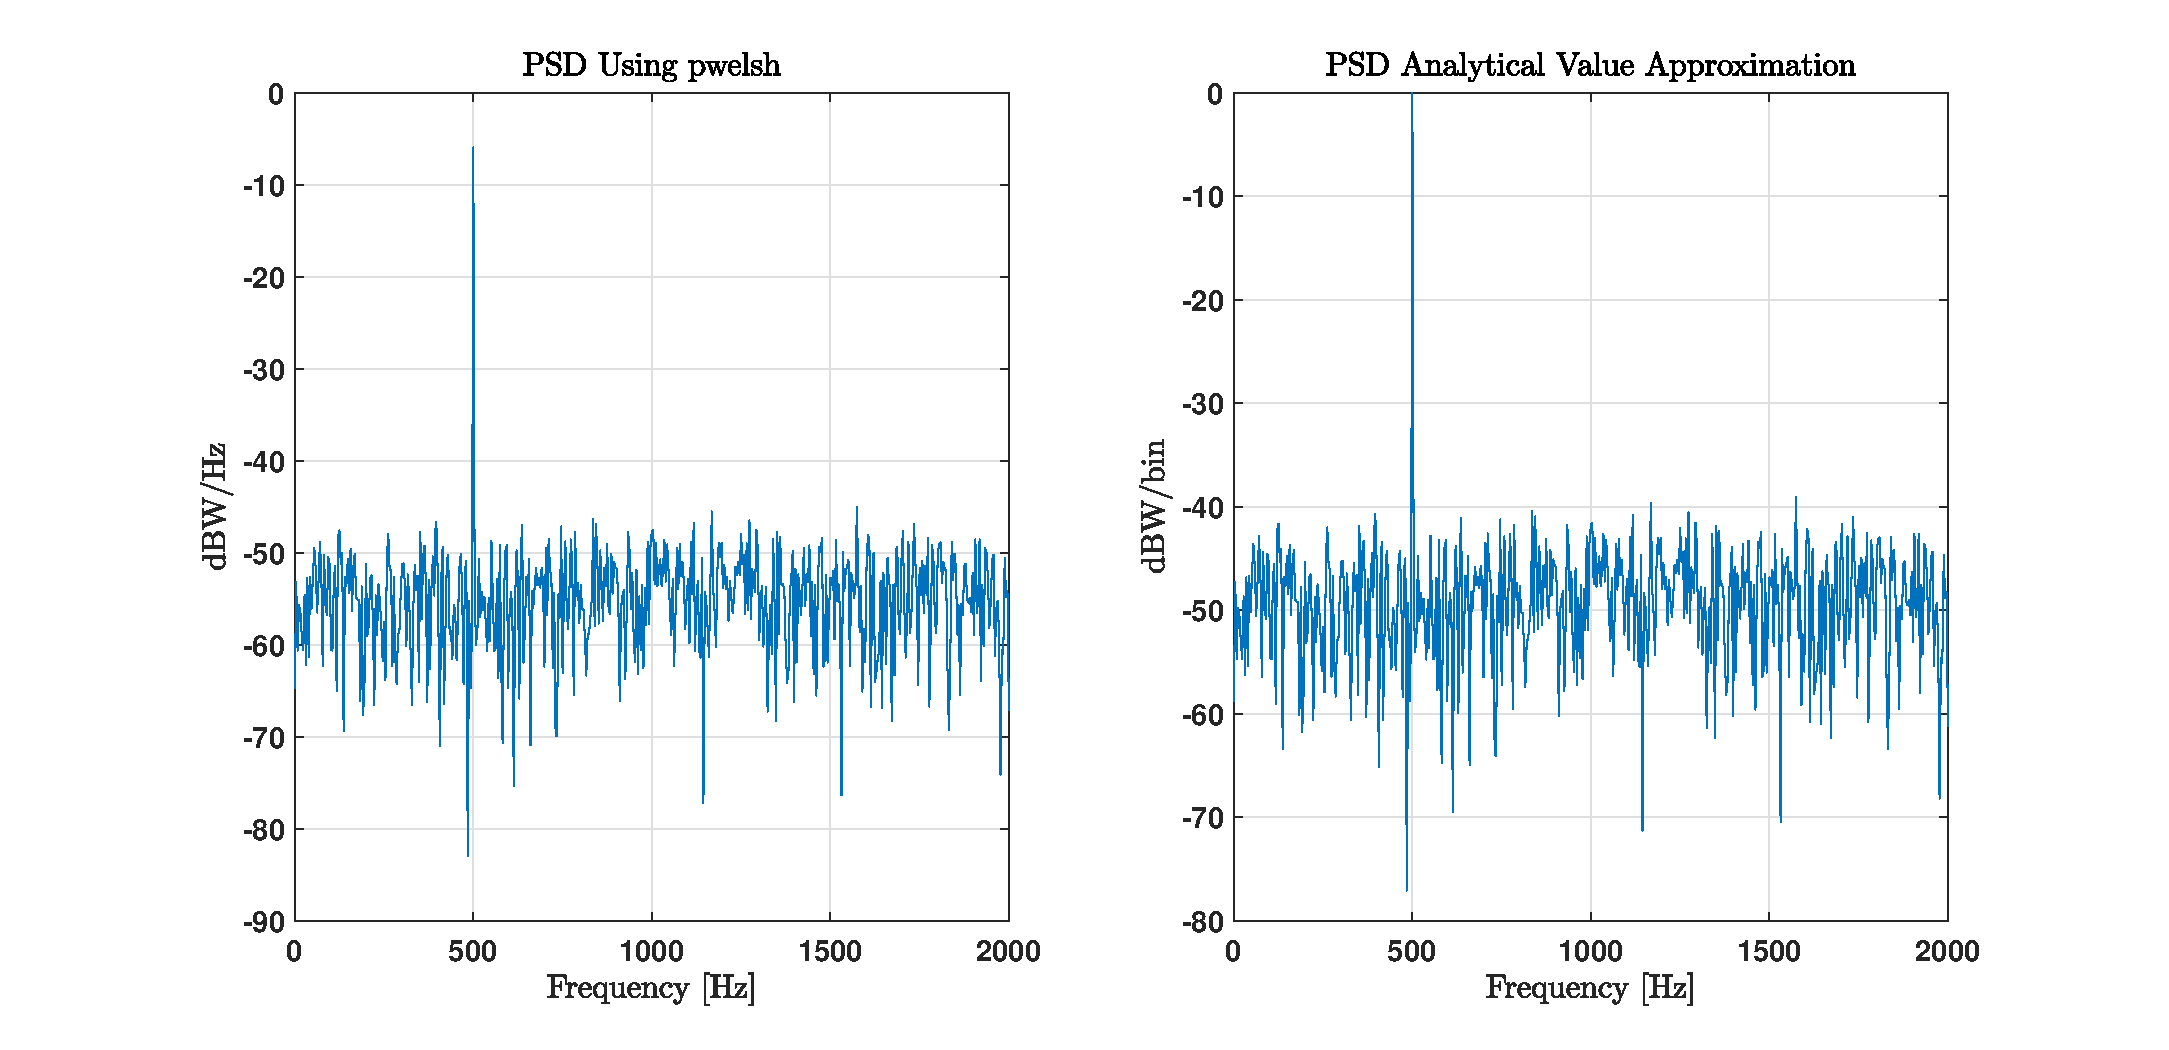
\includegraphics[scale=0.5]{Figures/PSD_Com/Demo_PSD_Sin}
\caption{Sin Demo using pwelsh function}
\label{fig:PSD_Com:Demo_PSD_Sin}
\end{figure}

The result of the \verb|pwelsh|, which is \verb|10log10(pxx)|, give a value of $\approx$ -5.9 dBW, which is different from 0 dBW.\\

So how to move from -5.9 dBW $\rightarrow$ 0 dBW ?

What we need to do is to multiply the value of \verb|pxx|, which is W/Hz, and convert to Watt/bin, and this done as:

\begin{equation}
 \text{Pbin (W/bin) = pxx (W/Hz) * Fs/nfft (Hz/bin)}
\end{equation}

\subsection{Windowing,Overlapping}

\todo{PSD:Windowing,Overlapping}.

\newpage
\section{Equivalent noise bandwidth(ENBW)}

\begin{itemize}

\item \underline{source:} \url{https://analog.intgckts.com/equivalent-noise-bandwidth/}.

Contains nice definition, and graphics

\item  MATLAB source for simulation: \url{https://fr.mathworks.com/help/signal/ref/enbw.html#btrihsq-1}

\end{itemize}

\todo{ENBW} \underline{\textit{ENBW}:} \textit{To redo a proper documentation and simulation from the resources above}. 


\chapter{FIR}

\section{Window Method}

\subsection{Low Pass Design}

In this example, we design a low pass FIR filter using 2 windows: rectangular and Hamming.\\

The rectangular provides the best transition bandwidth, but has unacceptable ripples in the pass band and the stop band, so we use Hamming window to adjust these unacceptable ripples in the expense of a wider transition bandwidth.\\

The design specifications are:

\begin{itemize}
    \item Order: 24
    
    \item Normalized cuttoff frequency: 0.5
\end{itemize}

\newpage
Results are in \autoref{fig:FIR_Sim:FIR_lowpass_rect_Hamm_window}.

\begin{figure}[ht]
\centering
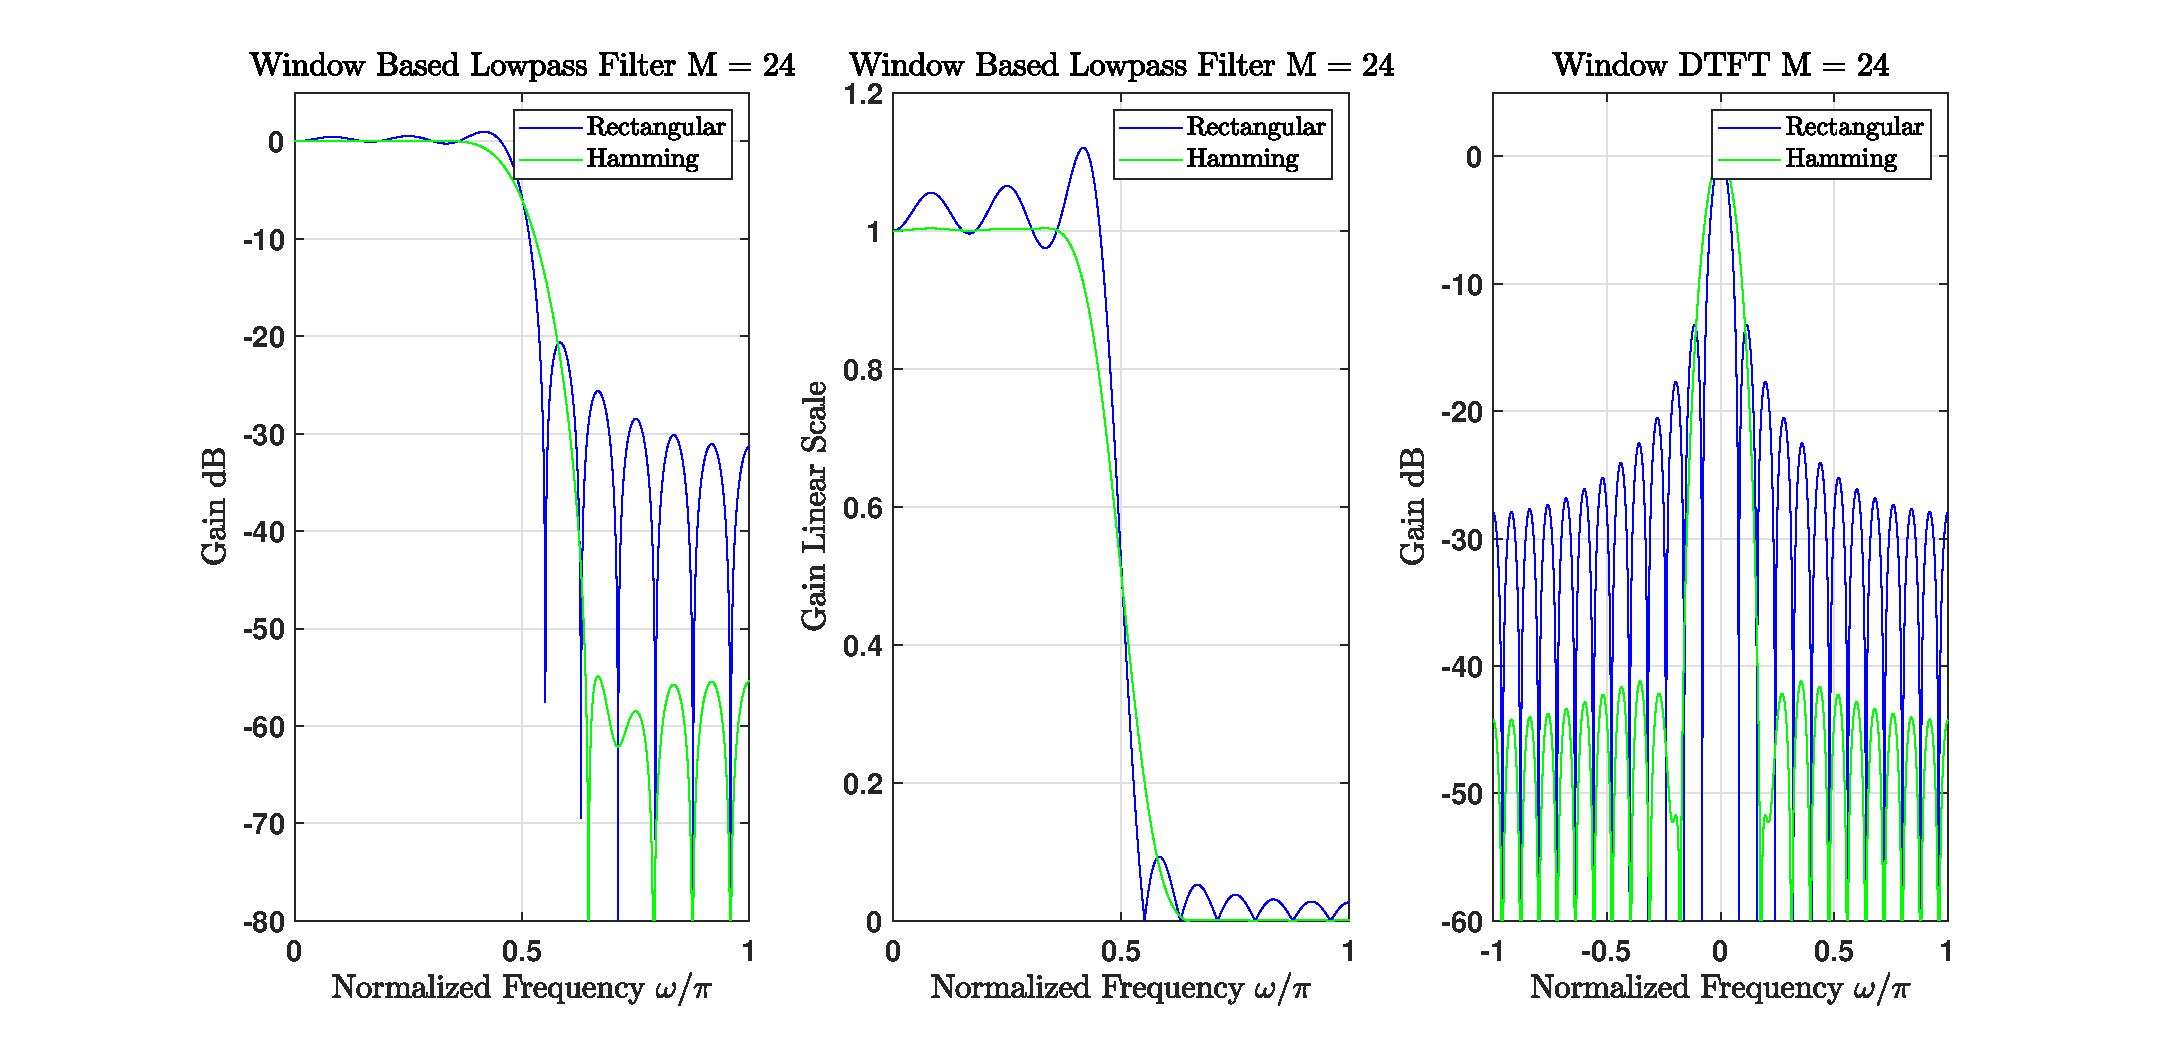
\includegraphics[scale = 0.5]{Figures/FIR_Sim/lowpass_window_method.eps}
\caption{FIR Low pass example using Rectangular and Hamming window}
\label{fig:FIR_Sim:FIR_lowpass_rect_Hamm_window}
\end{figure}

\begin{itemize}
    \item For Hamming window:
    
        \begin{itemize}
            \item Main lobe width is $\displaystyle\frac{8 \pi}{M}$ where $M$ is the filter order in this case
            
            \item Peak side lobe is -41 dB
        \end{itemize}
    
    
\end{itemize}

\subsection{Bandpass Design}

Now we will do a banpass design using the following specs shown in \autoref{fig:FIR_Sim:bandpass_example_given}

\begin{figure}[ht]
\centering
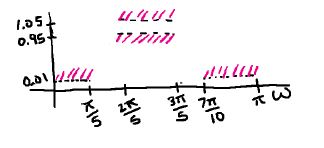
\includegraphics[scale = 0.7]{Figures/FIR_Sim/bandpass_example_given}
\caption{Bandpass Design Example}
\label{fig:FIR_Sim:bandpass_example_given}
\end{figure}

\begin{itemize}
    \item In the $\mathrm{1}^\mathrm{st}$ stop band, the transition bandwidth is $\displaystyle\frac{2 \pi}{5} \, - \, \displaystyle\frac{\pi}{5} \, = \, \displaystyle\frac{ \pi}{5}$
    
    \item In the $\mathrm{2}^\mathrm{nd}$ stop band, the transition bandwidth is $\displaystyle\frac{7 \pi}{10} \, - \, \displaystyle\frac{3\pi}{5} \, = \, \displaystyle\frac{ \pi}{10}$
    
    
    \item So as a result and specification we choose the smaller transition bandwidth that is $\displaystyle\frac{ \pi}{10}$
    
    \item As a deviation error, we have  $0.01 < 0.05$, so we take 0.01 as the error to be computed in the stopband and the bandpass
    
    
\end{itemize}

The window to be chosen for the specification is the Kaiser window, which depends upon 2 parameters:

\begin{enumerate}
    \item $\beta$ which controls the window shape: if $\beta \, = \, 0 \rightarrow$ rectangular window, and if $\beta$ increase then the mainlobe width increase and the sidelobe height decrease
    
    \item $M$ for the transition bandwidth
    
\end{enumerate}

\newpage
Results are shown in \autoref{fig:FIR_Sim:bandpass_Kaiser_results} and \autoref{fig:FIR_Sim:bandpass_example_error_plot}.

\begin{figure}[ht]
\centering
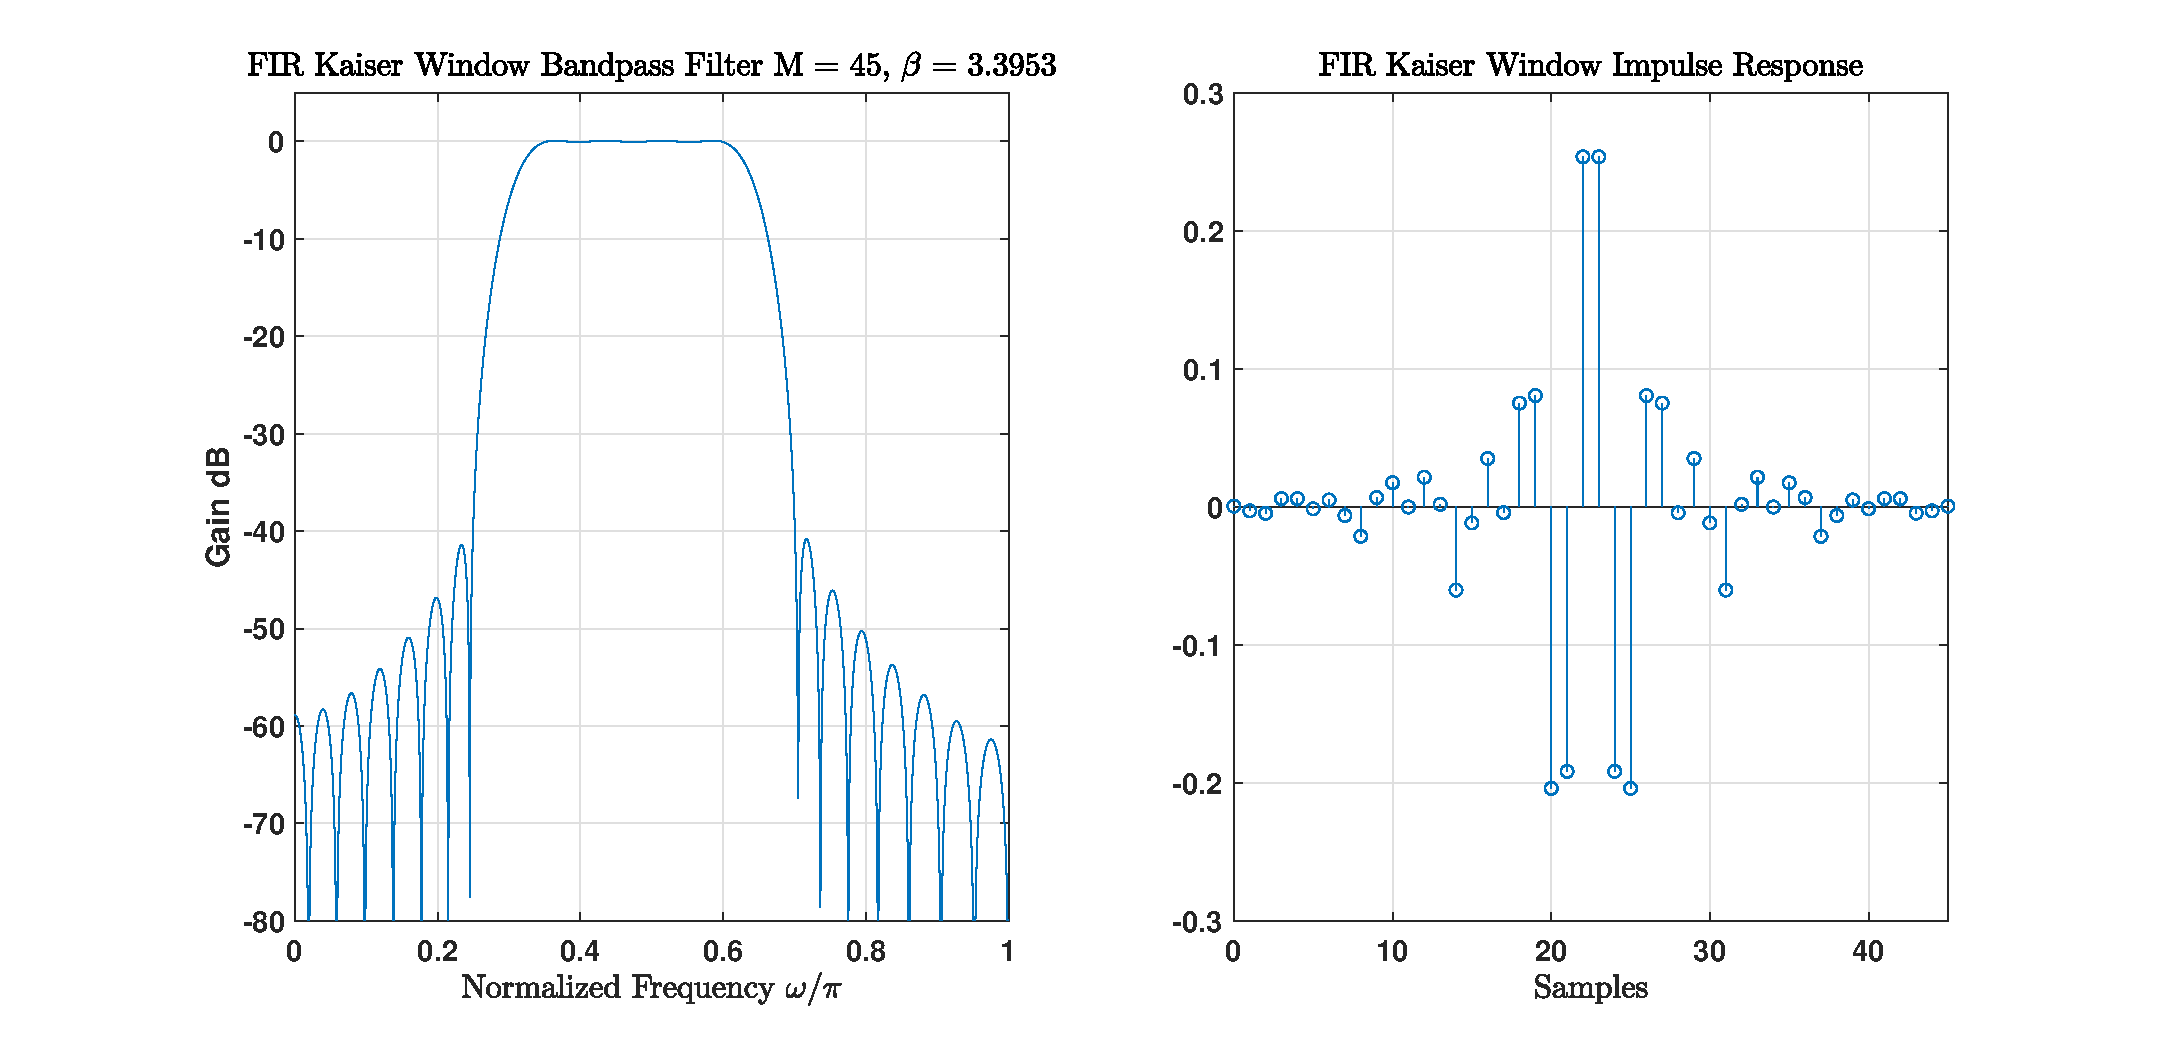
\includegraphics[scale = 0.5]{Figures/FIR_Sim/Bandpass_window_Kaiser.eps}
\caption{Bandpass Design Results for Kaiser Window}
\label{fig:FIR_Sim:bandpass_Kaiser_results}
\end{figure}

\begin{figure}[ht]
\centering
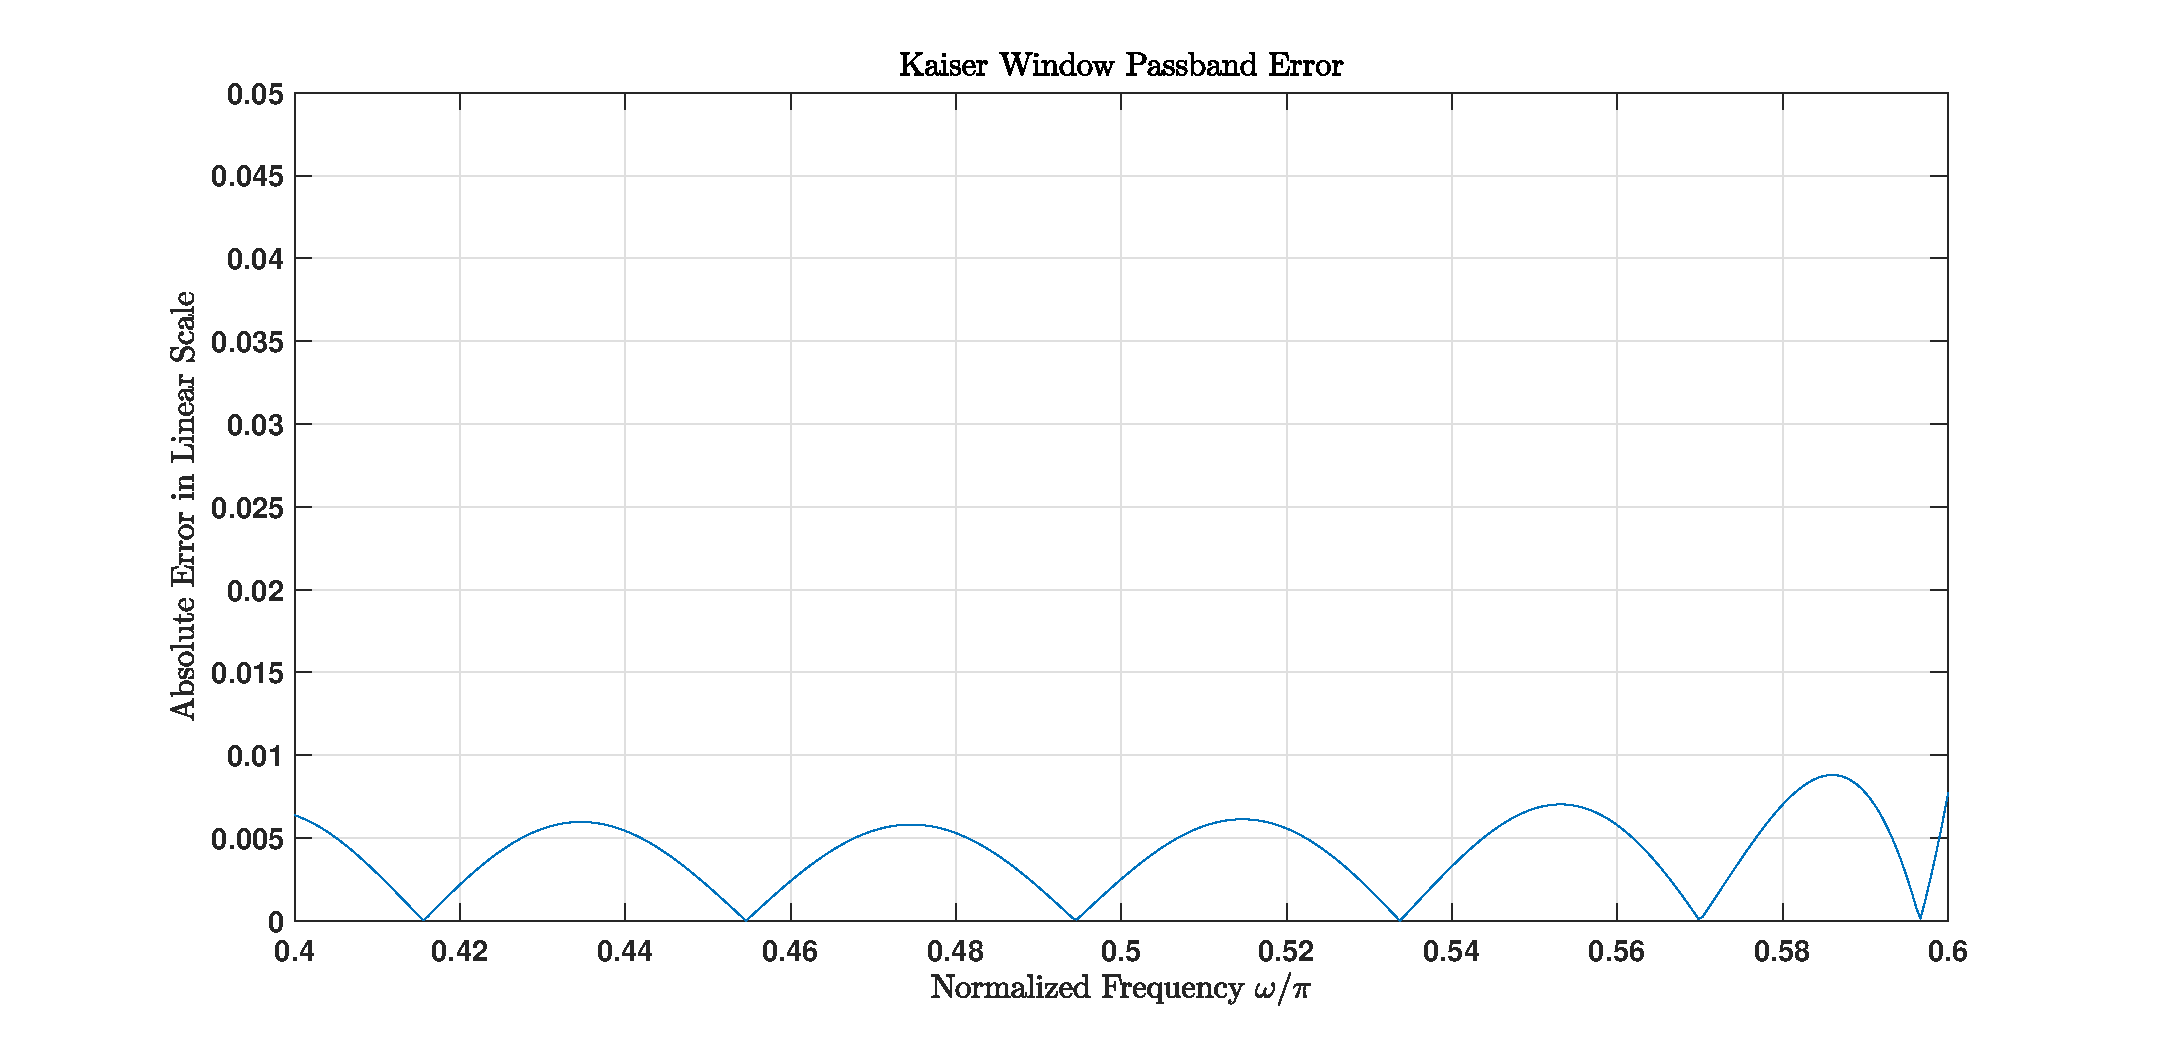
\includegraphics[scale = 0.3]{Figures/FIR_Sim/Bandpass_window_Kaiser_error_deviation.eps}
\caption{Bandpass Design Results for Kaiser Window: Error is less then 0.01}
\label{fig:FIR_Sim:bandpass_example_error_plot}
\end{figure}


\newpage
\section{Frequency Sampling Method}



\subsection{Low Pass Example}

The specifications are: 

\begin{itemize}

\item $\omega_{\text{pass}} \, = \, 0.25 \pi \, , \, \omega_{\text{stop}} \, = \, 0.35 \pi $

\item $  A_p \, = \, 0.1 \text{ dB} \, , \, A_s \, = \, 40 \text{ dB}$

\item By result the transition bandwidth is $\Delta \omega \, = \, \omega_{\text{pass}} \, - \, \omega_{\text{stop}} \, =  \, 0.35 \pi - \, 0.25 \pi  \, = \, 0.1 \pi$  


\end{itemize}


For a rectangular window as interpolating function, we have $\Delta \omega \, = \, \displaystyle\frac{4 \pi}{L} \rightarrow \, L \, = \, 40 \, = \, M \, + \, 1 $, so we need to begin with an \tbi{FIR of length at least 40} (order 39).\\



\begin{figure}[ht]
\centering
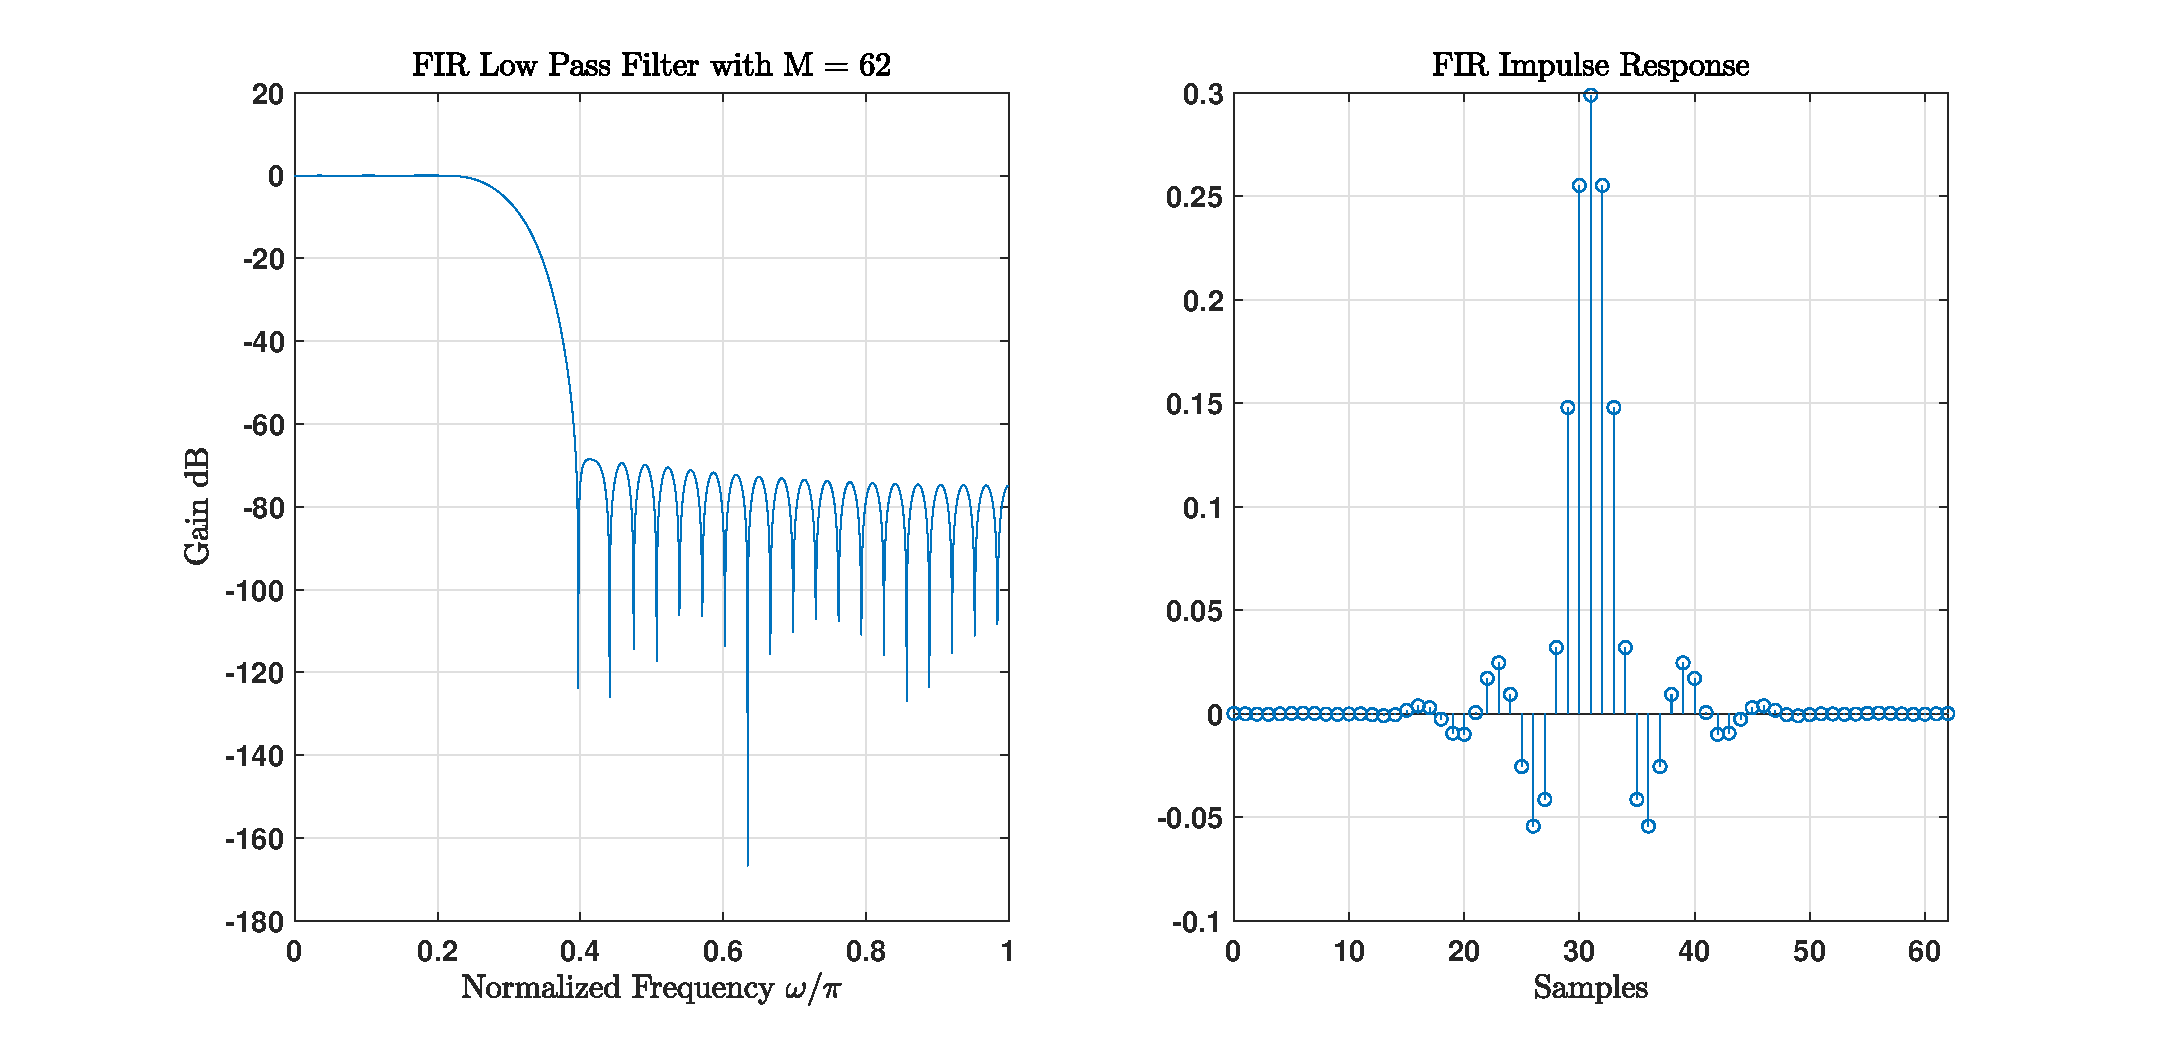
\includegraphics[scale = 0.4]{Figures/FIR_Sim/lowpass_freqsampling_method.eps}
\caption{FIR Low Pass with an order of $M\, = \, 62$}
\label{fig:FIR_Sim:lowpass_freqsampling_method}
\end{figure}



\todo{To do}:

\begin{itemize}

\item Write the formula and the design criteria

    \begin{itemize}
        \item Eq of FIR
        
        \item Steps of design in window method
        
        \item Concepts and techniques in designing
        
        \item Implementation using toolbox and from scratch
        
        \item Repeat the examples using toolbox and implementation using OOP style
        
        
    \end{itemize}

\end{itemize}


\chapter{Matched Filter}

\section{Intro and Recap}


Before simulation we will do a recap about matched filter principles (oriented in communication application).\\

Imagine we have some bits to be transmitted (1 is encoded as 1 volt and 0 as -1 volt), where these bits are passed through a pulse shaping filter (we will assume we have a square pulse wave for a period of $T_{\text{bit}}$).\\

\todo{Block diagram:} \underline{\textit{Block diagram:}}  \textit{To insert a block diagram of the intuition later}.\\

These pulses will pass through a channel, and will have some gain $G$ and some additive noise $n(t)$. \\ 

\underline{Question:} How do we know if we receive a +1 or -1 ?\\

\underline{Answer:} Well, we have to collect all the energy through the pulse, that's why we need to design a filter $h(t)$ which do this, and \textit{then} sample its output at multiple time of $T_{\text{bit}} \leftrightarrow t = K \, T_{\text{bit}}$.\\

The following fact (without the proof) are to be remembered:

\begin{itemize}

\item The best $h(t)$ is to be known $s(T_{\text{bit}} \, - \, t)$: that is the same pulse shape, but flipped in time and then time shifted by $T_{\text{bit}}$

\begin{itemize}
    \item As a matter of fact, the formal definition of a matched filter: it is a filter designed to maximize the SNR $\rightarrow$ the SNR will be maximized at the communication (or any system we use it)

\end{itemize}

\item  For a square pulse $s(t)$ for example, $h(t)$ will be also a square wave for this particular case. The result of a convolution of 2 square wave will be a triangular wave of period $2 \, T_{\text{bit}}$.

\item  for other pulses, we will have also triangles but shifted

\item  At each peak time, we will not have a contribution from other triangles $\rightarrow$ which means that we don't have contribution from other pulses, and only current pulse is contributing


\end{itemize}







%*****************************************************
%*****************************************************
%*****************************************************


\chapter{Bandpass Sampling}

\section{Non Integer Band Positioning}

\subsection{Reminder}

\underline{Source:} see section 2-3 in \cite{book_understanding_dsp}.

\begin{itemize}
    \item In bandpass sampling, we are interested in bandwidth rather the highest frequency component in the spectrum
    
    \item Sampling rate bounds to respect \cite{book_understanding_dsp}:
    
    \begin{equation}
\displaystyle\frac{2 \, f_{\text{center}} \, + \, B}{m} \, \leq \, F_s \, \leq \, \displaystyle\frac{2 \, f_{\text{center}} \, - \, B}{m \, - \, 1}
\end{equation}

such that $m \in \mathbb{N}$ represent the number of replica.    
\end{itemize}

\subsection{Simulation}



%*****************************************************
%*****************************************************
%*****************************************************


\chapter{Introduciton to Multirate Signal Processing}

\section{Donwsampling}

What happen to the time frequency index when doing downsampling.\\

From frequency sampling and DFT computations, we know that when computing a frequency bin numerically, the frequency step is $\displaystyle\frac{2 \pi}{N}$, where $N$ is the total number of samples (the length of the discrete time signal or the sampled signal).\\

So we have the relation:

\begin{equation}
f \, \times \, t \, \leftrightarrow \, n \, \times \,  \displaystyle\frac{k}{N}
\end{equation}

where:

\begin{itemize}
    \item $f$ and $t$ are some indexes for continuous frequency and time 
    
    \item $n$: discrete time index
    
    \item $k$: discrete frequency index
\end{itemize}

When we downsample by a factor of $D$, the relation between the indices is:
\begin{equation}
\displaystyle\frac{k \, n}{N} \leftrightarrow   \displaystyle\frac{k \, n}{N/D}
\end{equation}

Also recall that $F_s \geq \, 2 \, f$, but a more equivalent common form is $f \leq \, \displaystyle\frac{F_s}{2}$, which mean the analog baseband frequency is captures between the range 0 to $\displaystyle\frac{F_s}{2}$. So we can say:

\begin{equation}
  F_s \geq \, 2 \, f \, \equiv  f \leq \, \displaystyle\frac{F_s}{2} 
\end{equation}

\newpage
\underline{What happen when we downsample?}\\

If we begin with a signal with a sampling rate $F_s$, where the CTFT spectrum contains $N$ point ($N$ is the total number of samples with a sampling period $T_s \, = \, \displaystyle\frac{1}{F_s}$).\\

Let's take an example of a sin wave, where its CTFT spectrum is shown in \autoref{fig:Multirate:sin_wave_CTFT}.


\begin{figure}[ht]
\centering
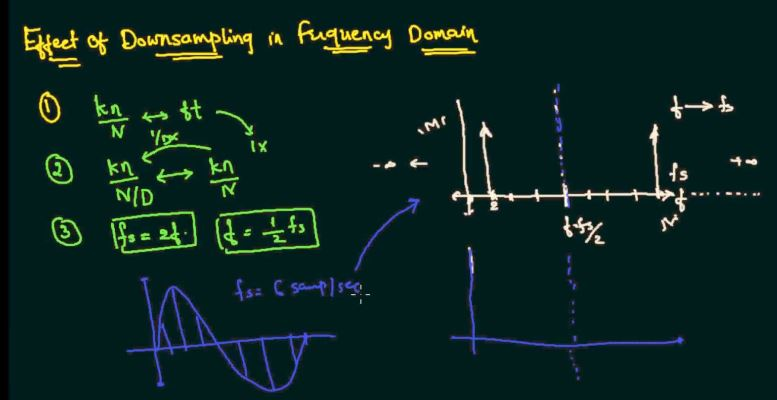
\includegraphics[scale = 0.5]{Figures/Multirate/sin_wave_CTFT}
\caption{Sine Wave CTFT Spectrum}
\label{fig:Multirate:sin_wave_CTFT}
\end{figure}

The original $F_s \, = \, 6 Hz$, that is 6 sample per cycle (this in the time domain), and the DFT spectrum for the CTFT contains $N \, = \, 6$ frequency fundamental points (for a window duration of 1s let's say).\\

\newpage
If we downsample and let the new $F_s$ 3 Hz, that is $F_s^D \, = \, 3$ Hz, we will have:

\begin{itemize}
    \item 3 samples per cycle (period) instead of 3 $\leftrightarrow$ time domain effect
    
    \item Frequency domain effect (see \autoref{fig:Multirate:sin_wave_CTFT_downsample}):
    
        \begin{itemize}
        
        \item Folding line $\displaystyle\frac{F_s}{2}$ will get closer
        
        \item Frequency points indices will also get lost because $N$ is reduced , but the frequency index 2 remain fix $\leftrightarrow$ so the spectrum get preserved
        \end{itemize}
    
\end{itemize}

\begin{figure}[ht]
\centering
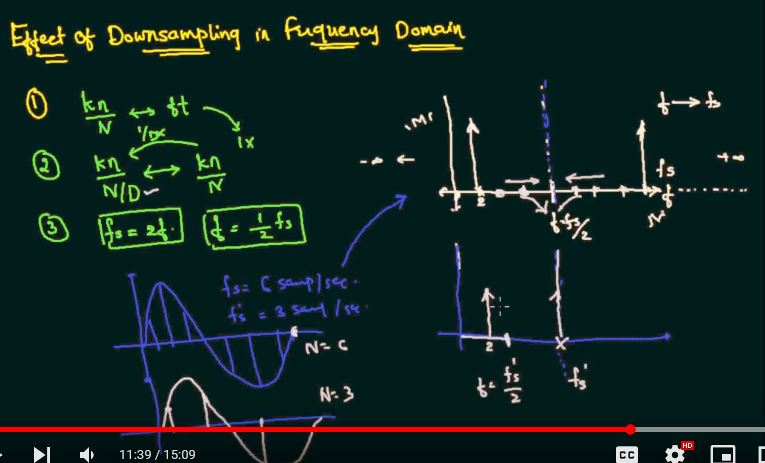
\includegraphics[scale = 0.5]{Figures/Multirate/sin_wave_CTFT_downsample}
\caption{Sine Wave CTFT Spectrum}
\label{fig:Multirate:sin_wave_CTFT_downsample}
\end{figure}

Important note: if we do dowsanmpling, it is not necessarily that aliaising get occurred.\\

A more general example for a bandlimited signal is shown in \autoref{fig:Multirate:CTFT_bandlimited_downsample} 

\begin{figure}[ht]
\centering
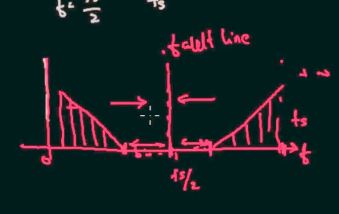
\includegraphics[scale = 0.8]{Figures/Multirate/CTFT_bandlimited_downsample}
\caption{Sine Wave CTFT Spectrum}
\label{fig:Multirate:CTFT_bandlimited_downsample}
\end{figure}

When we downsample, the folding line $\displaystyle\frac{F_s}{2}$ will get closer (move to the left). As long as the new folding line $\displaystyle\frac{F^D_s}{2} \ \, > \, f_{max}$, the signal spectrum is preserved and no aliasing occur.

\subsection{Example: Downsampling with no aliasing}


\todo{dowsampling with no aliasing}: to redo with a sinc example.

We take a numerical example to illustrate downsampling.\\

First we generate a bandlimited signal with a bandwidth of 100 Hz, generated using the \verb|fir2| command.\\

The $\omega_{\text{pass}} \, = \, 0.25 \pi$, and the correspondent analog frequency $f_{\text{pass}} \, = \, \omega_{\text{pass}} \, \times \, F_s \, \times \, \frac{1}{2 \pi} \, = \, 100 Hz$.\\


The initial sampling rate $F_s^{\text{init}} \, = \, 800 Hz$, and we downsample by a factor 4, so the new sampling rate $F_s^{D} \, = \, \displaystyle\frac{F_s^{\text{init}}}{D} \, = \, \displaystyle\frac{800}{4} \, = \, 200 $ Hz.\\

Notice that new folding line now is $ \displaystyle\frac{F_s^{D}}{2} \, = \, 200 > \, 100$, where the 100 is the bandwidth of the signal, so no aliasing will occur and the bandwidth will still the same.

\newpage
\section{Downsampling with Aliasing}

\underline{Note:} this section contains many simulations and explanation, and since they have allot of details and contain many points, I decided to make it as a section instead of a subsection.\\ 


\subsection{Example 1: Aliased Sin and Cos}
\label{Sub:Downsampling_Aliasing}

\underline{Ref:} chapter 11 in \cite{book_Li_Tan_dsp_fundamentals_and_app}.\\

We take 1 cos and sin signal as the following:

\begin{equation}
    x(t) \, = \, 5 \sin(2 \, \pi 10^3 \, t ) \, + \, \cos(2 \, \pi \, 2.5 \, \times \, 10^3 \, t)
\end{equation}

\begin{itemize}
    \item Frequency of each component is at 1 KHz and 2.5 KHz
    
    \item $F_s \, = \, 8$ KHz
\end{itemize}

For $F_s \, = \, 8$ KHz, the folding frequency is at $\displaystyle\frac{F_s}{2} \, = \, 4$ KHz $> 2.5 $KHz, so no aliasing occur.\\

Let's say we downsample by a factor $D \, = \, 2$, so we will have:

\begin{itemize}
    \item $F_{s_D} \, = \, \displaystyle\frac{F_s^{\text{orig}}}{D} \, = \, \displaystyle\frac{8000}{2} \, = \, 4$ KHz
    
    
    \item The new folding frequency will be $\displaystyle\frac{4000}{2} \, = \, 2000$ Hz  $ < \, 2500$ Hz
    
\end{itemize}

In this case, the new folding frequency is smaller then the bigger frequency component in $x(t)$, so aliasing will occur in the reconstructed signal.\\

\newpage
\underline{Computation of the aliased frequency:}\\

The alias frequency will be smaller then the new sampling rate $F_{sD} \, = \, 4$ KHz, and it can be computed as:

\begin{equation}
    \begin{array}{rcl}
        f_{\text{alias}} &=& \, F_{sD} \, - \,  f_{\text{max}}   \\
         &=& 4 \text{ KHz} \, - \, 2.5 \text{ KHz} \\
         &=& \, 1.5 \text{ KHz}
    \end{array}
\end{equation}


\begin{figure}[ht]
\centering
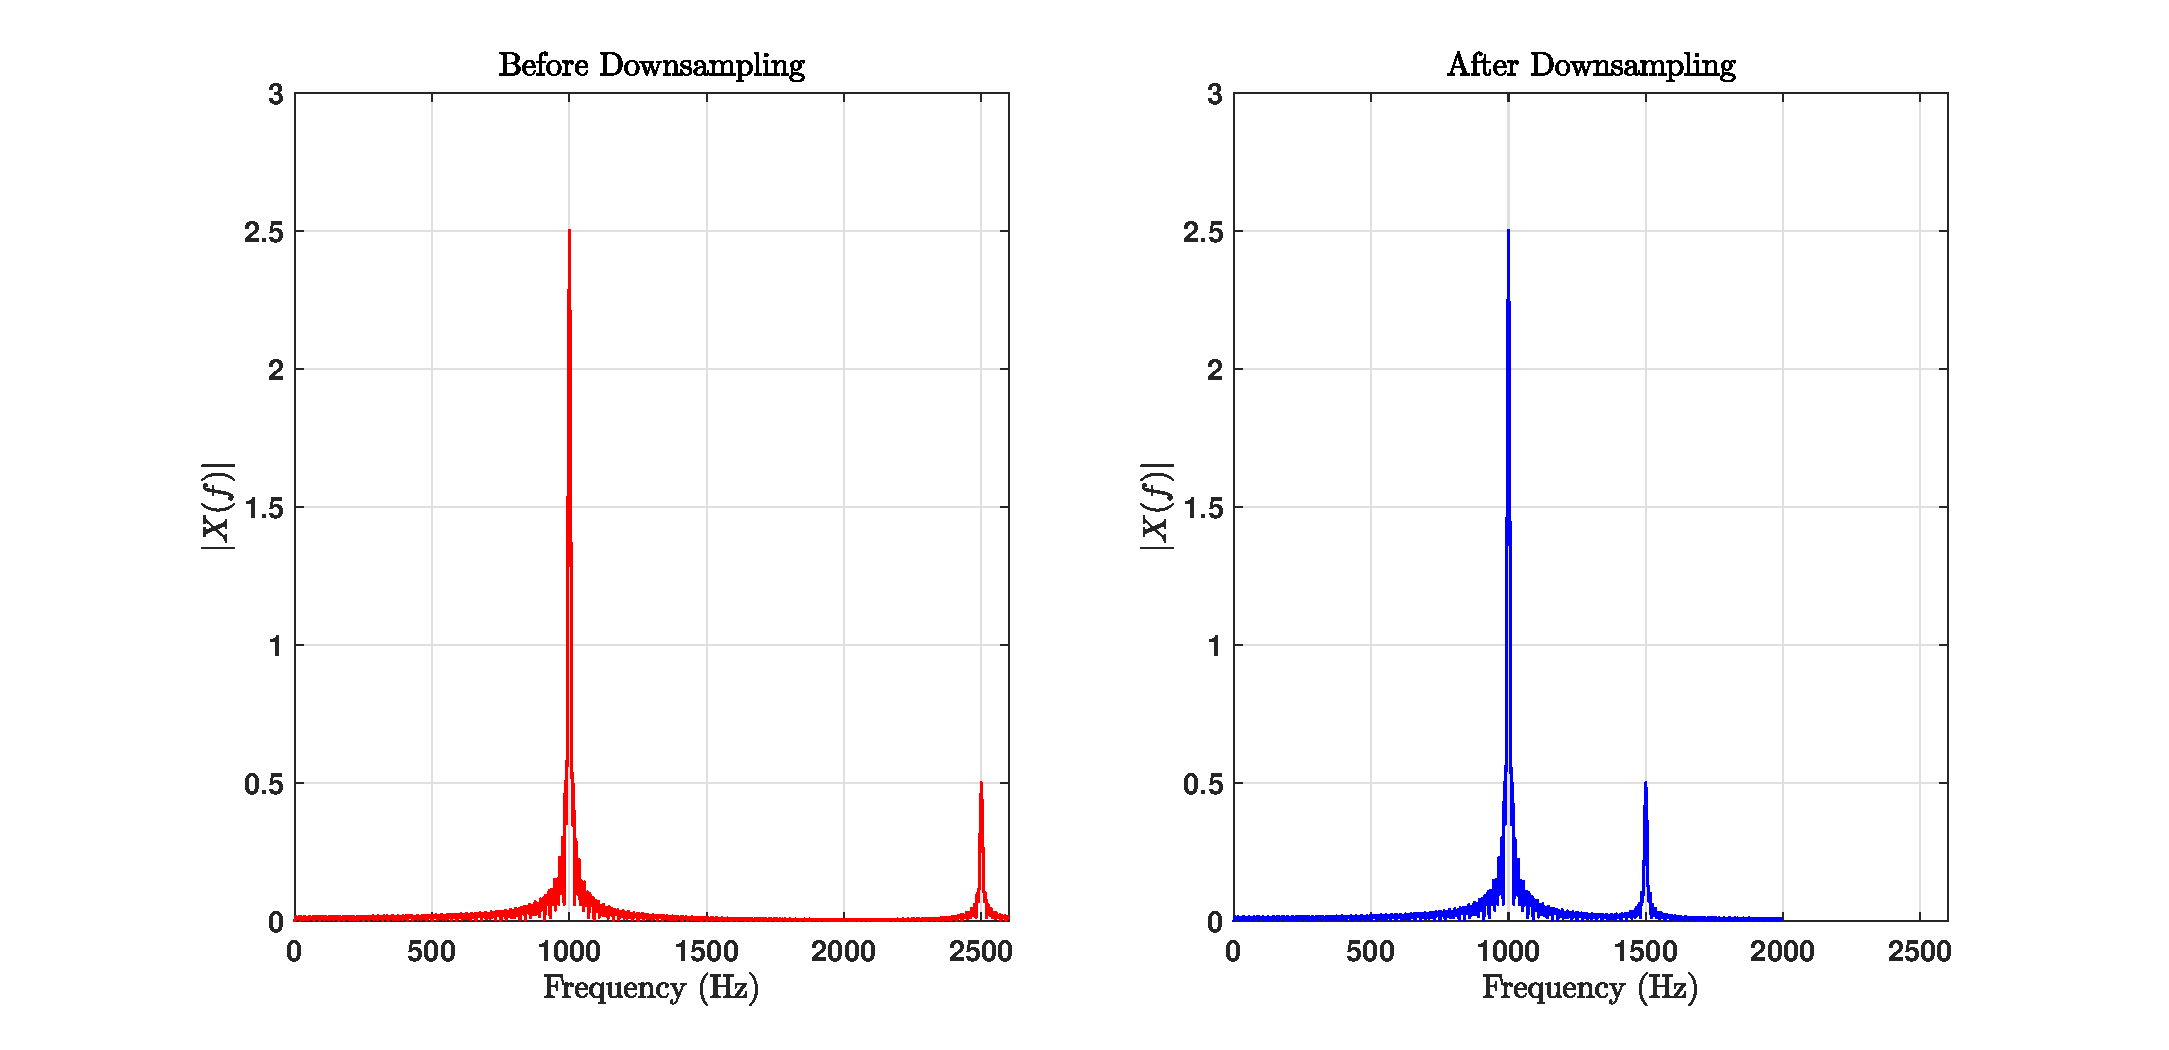
\includegraphics[scale = 0.5]{Figures/Multirate/a_Aliasing_Changing_Fs}
\caption{Sine Wave CTFT Spectrum}
\label{fig:Multirate:a_Aliasing_Changing_Fs}
\end{figure}


\underline{Example 2:}\\

In example 1, we have illustrated the aliasing by keeping the frequency of the signal constant and changing $F_s$, but also we can illustrate the aliasing by changing the frequency of the signal (like we have some signal generator with variable input frequencies) and keep $F_s$ constant.\\

\newpage
\subsection{Example 3: Aliasing with a full bandlimited signal}

Example 1 in \ref{Sub:Downsampling_Aliasing} focus on visualizing the aliasing with only sin (or cos) signals, or the sum of many sin.\\

The sin spectrum consist only of 1 peak at the location of frequency of the sin. Now we try to simulate the aliasing with signals where the spectrum extend from $0 \, \rightarrow \, B$[Hz].\\

\underline{Note of vocabulary:} by \textit{full bandlimited signal}, I mean that the amplitude spectrum is present over all the bandwidth $B$, not only over 1 frequency component like the sin or cos signals

So as example, we take the sinc signal.\\


\newpage
\subsubsection{Flow of the explanation}


\begin{itemize}

\item When I was try to debug the problem, I deiced to start with other test signal then sin or cos $\leftrightarrow$ signals that have only 1 frequency components


\item As a choice I took a sinc signal (See section 3.2.3 in \cite{sampling_beyond_band_limited_systems}):

\begin{equation}
  \text{sinc}\left(\,  \displaystyle\frac{t}{T}  \, \right) \, \leftrightarrow \, X(\Omega) \, = \, T \quad \text{ for } \displaystyle\frac{-\pi}{T} \, \leq  \, \Omega \, \leq \,  \displaystyle\frac{\pi}{T}  
\end{equation}

\item Parameters in simulation:

\begin{itemize}
    \item $B \, = \, 10$ Hz

    \item A \textit{big time window} from $-50 \rightarrow \, 50$ s
    
    \begin{itemize}
        \item So when simulating aliasing phenomena, I ensure that my source of error is only in low $F_s$ and not in a small time window
        
        \item Also I start before $t \, = \, 0$, so I don't assume causality of signal for now
        
    \end{itemize}
    
\end{itemize}

\item \underline{Result of Input Analog Signal:}

\begin{figure}[ht]
\centering
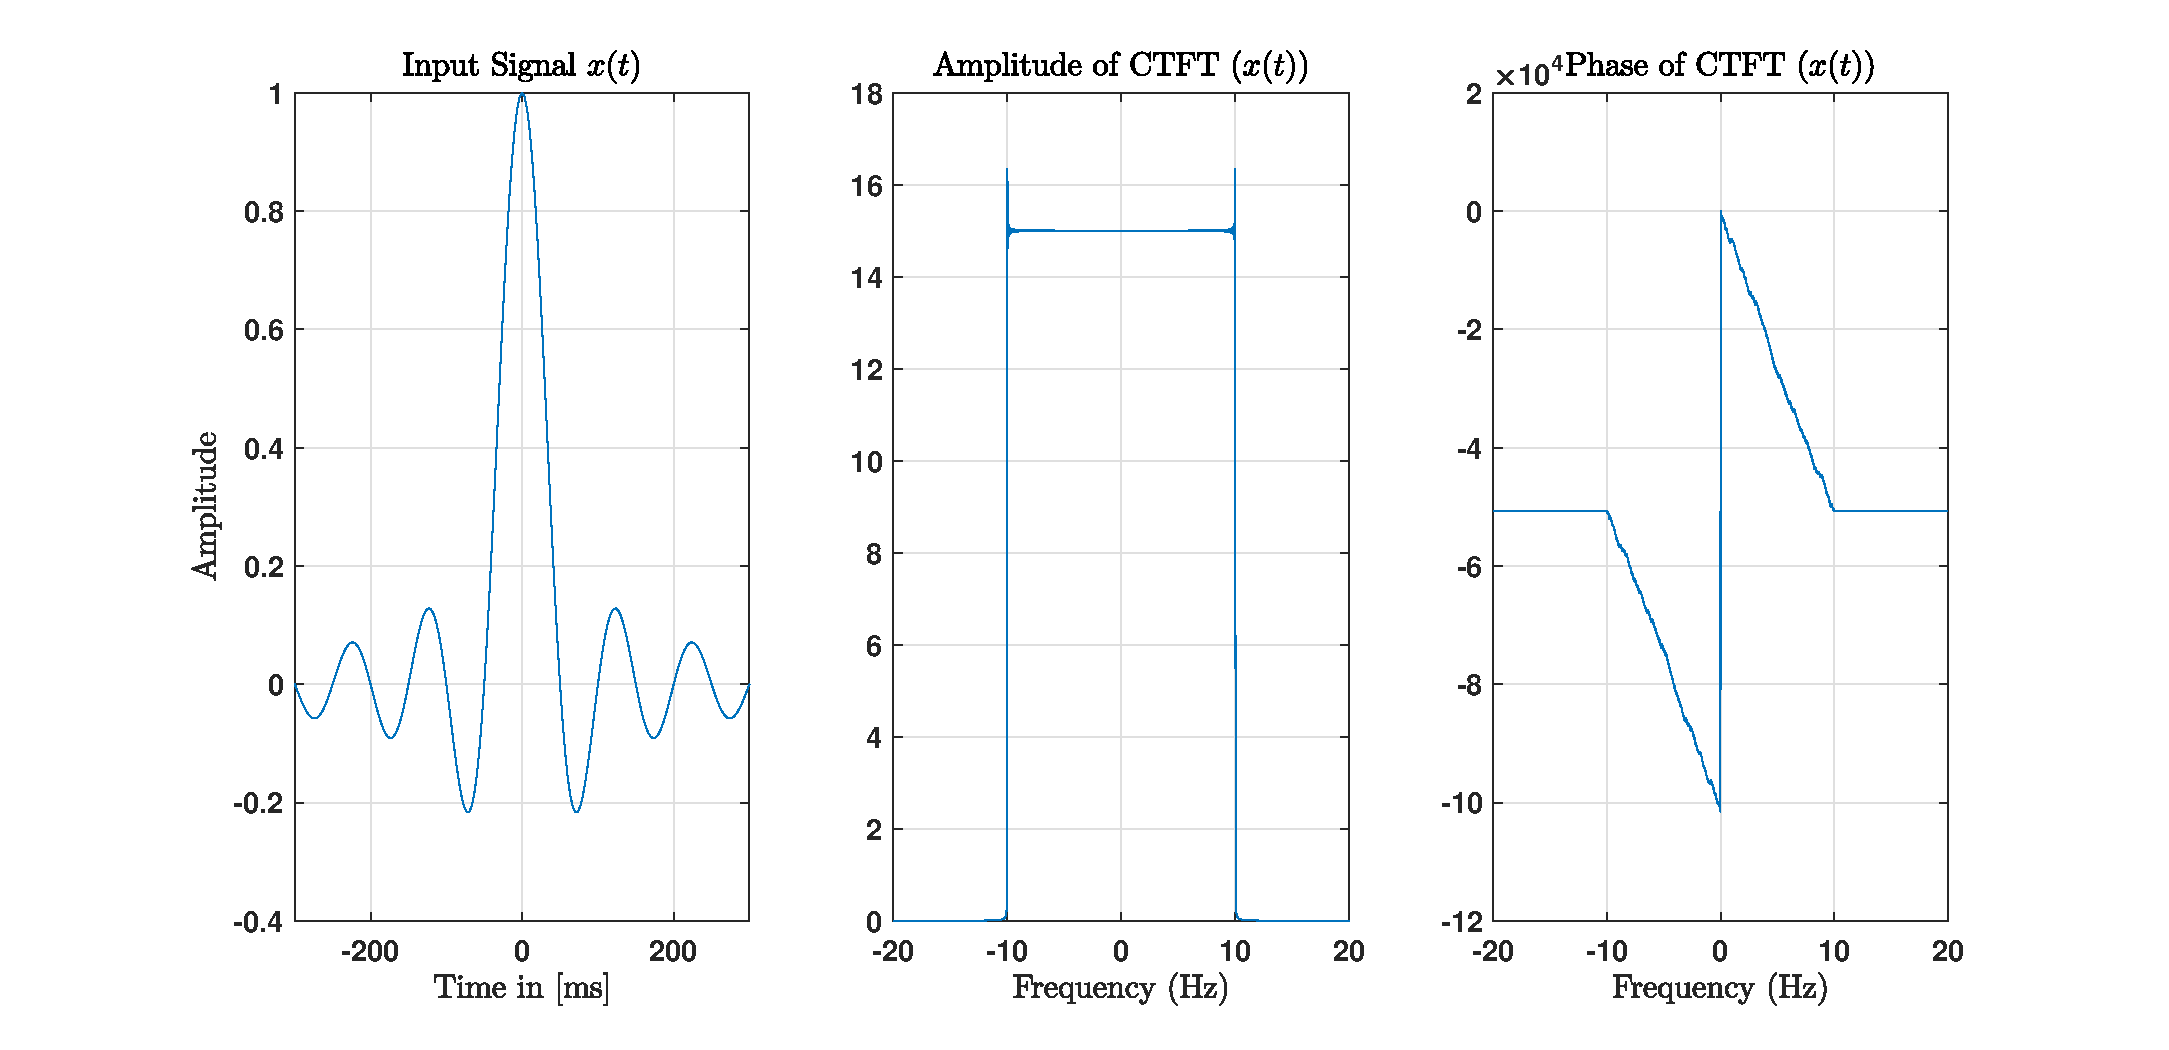
\includegraphics[scale = 0.5]{Figures/Sim_dowsampling_upsampling/Sinc_Input_Analog_B_10_Hz}
\caption{Input Analog Sinc signal}
\label{fig:Sim_dowsampling_upsampling:Sinc_Input_Analog_B_10_Hz}
\end{figure}


\begin{itemize}
    \item For analog simulation, I use oversampling to create a fine grid of analog time where $F_{s_{\text{analog}}} \,  = \, \text{oversampling } \times \, B$.
    
    In the code I took the oversampling $= \, 30 \rightarrow \, F_{s_{\text{analog}}} \, = \,300$ Hz
    
    \item For now I don't use any postprocessing (divide by the number of samples for example in a sin or a cos signal) for the FFT command to adjust the magnitude or the phase.
    
    I focus for now that the shape of the magnitude spectrum is correct with a correct bandwidth
    
   
\end{itemize}


\item To simulate any other $F_s$, I use \textit{integer} dowsampling operation where $D \, = \,\displaystyle\frac{F_{s_{\text{original}}}}{F_{s{\text{target}}}} \,  \in \mathbb{N} $ such that $ F_{s{\text{target}}}  \, < \, F_{s_{\text{original}}}$

\item To ensure my dowsampling operation is correct, I choose 2 $ F_{s{\text{target}}} \, = \, [60 \, , \, 30]$ Hz

\begin{itemize}
    \item Both $F_{s{\text{target}}} \, > \, F_{\text{Nyquist}} \, = \, 2 \, \times \, F_{H} \, = \, 20 $ Hz $\rightarrow$ no aliasing occur, and we will be able to do reconstruction 
\end{itemize}


\underline{Results:} CTFT Amplitude Spectrum

\begin{figure}[ht]
\centering
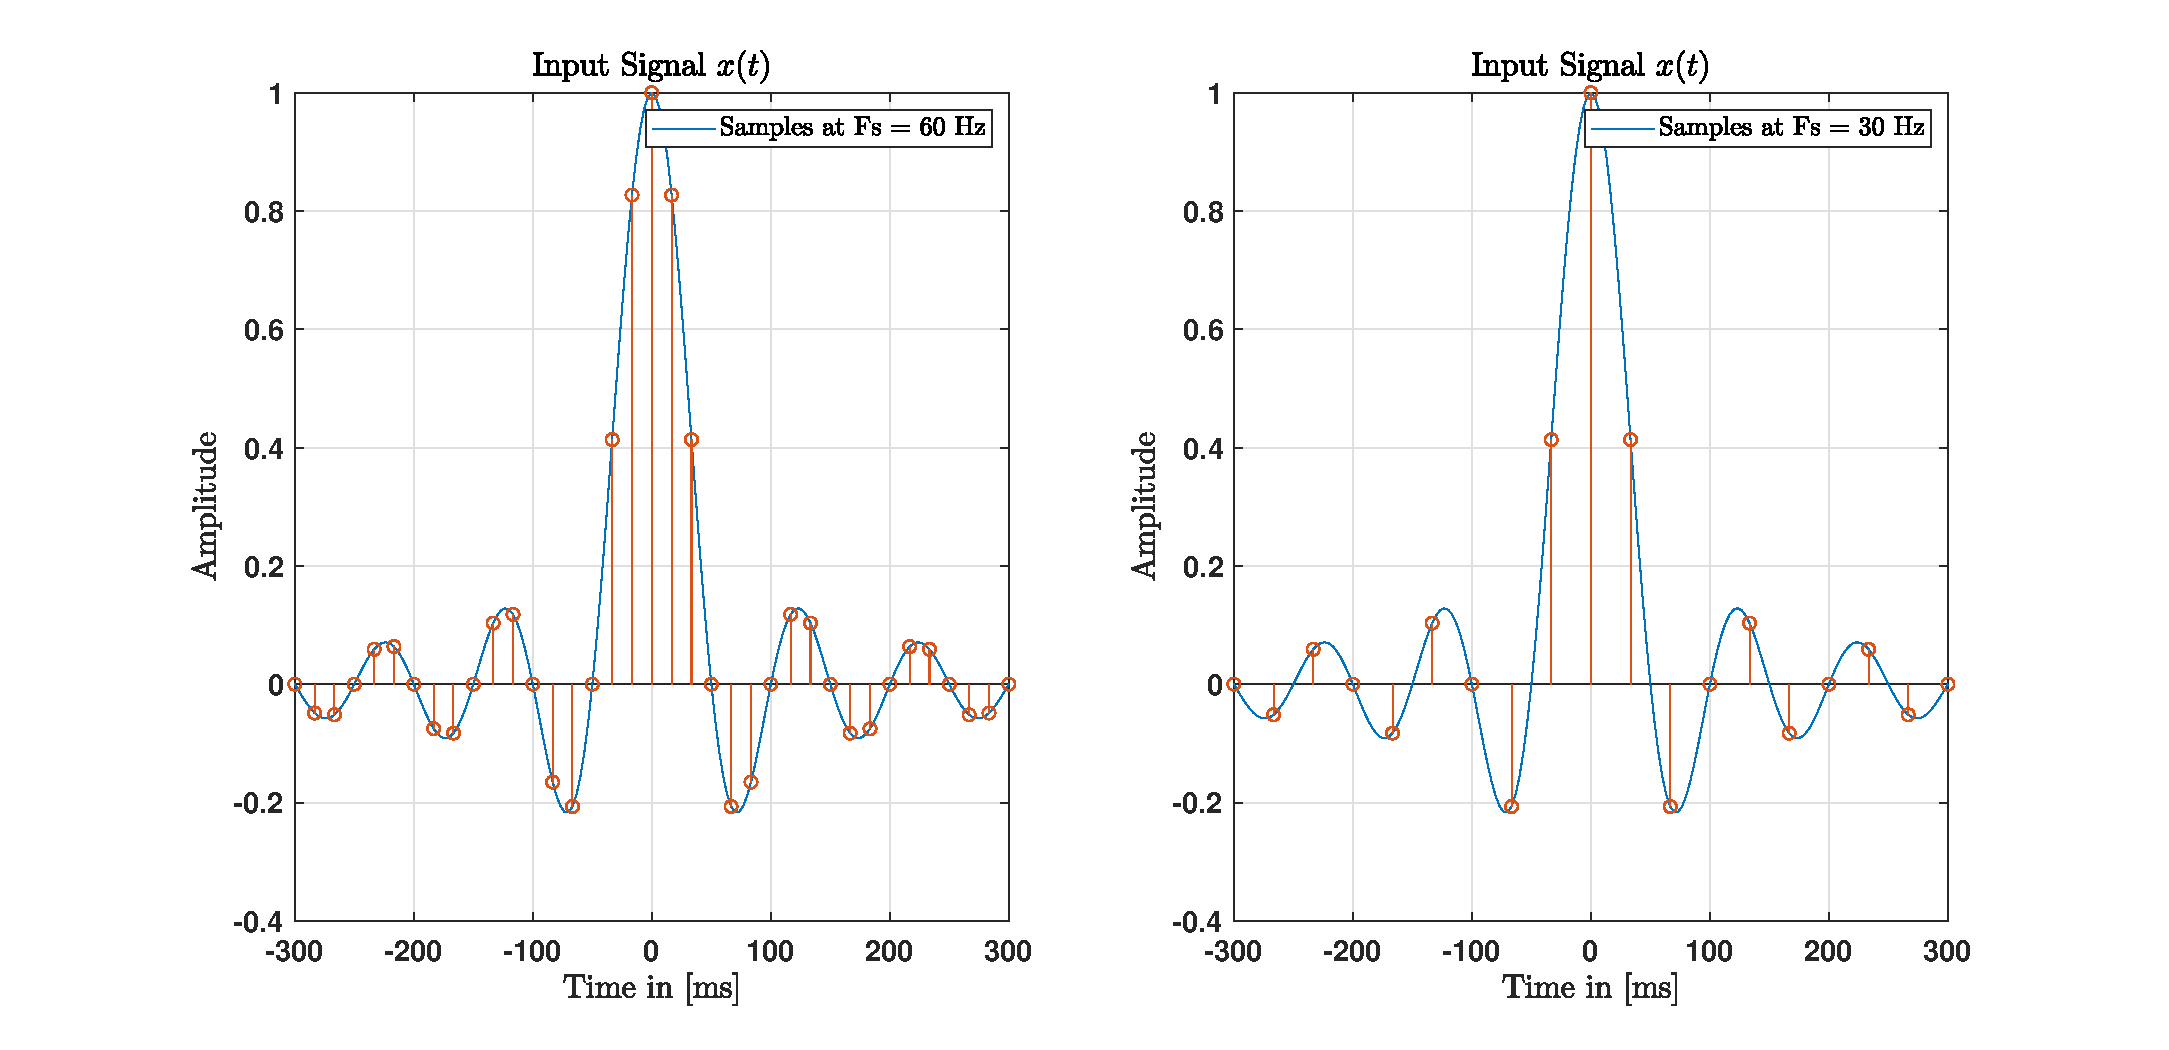
\includegraphics[scale = 0.4]{Figures/Sim_dowsampling_upsampling/downsample_sinc_Fs_30_and_60_Hz}
\caption{Ideal Reconstruction}
\label{fig:Sim_dowsampling_upsampling:downsample_sinc_Fs_30_and_60_Hz}
\end{figure}

\newpage

\begin{figure}[ht]
\centering
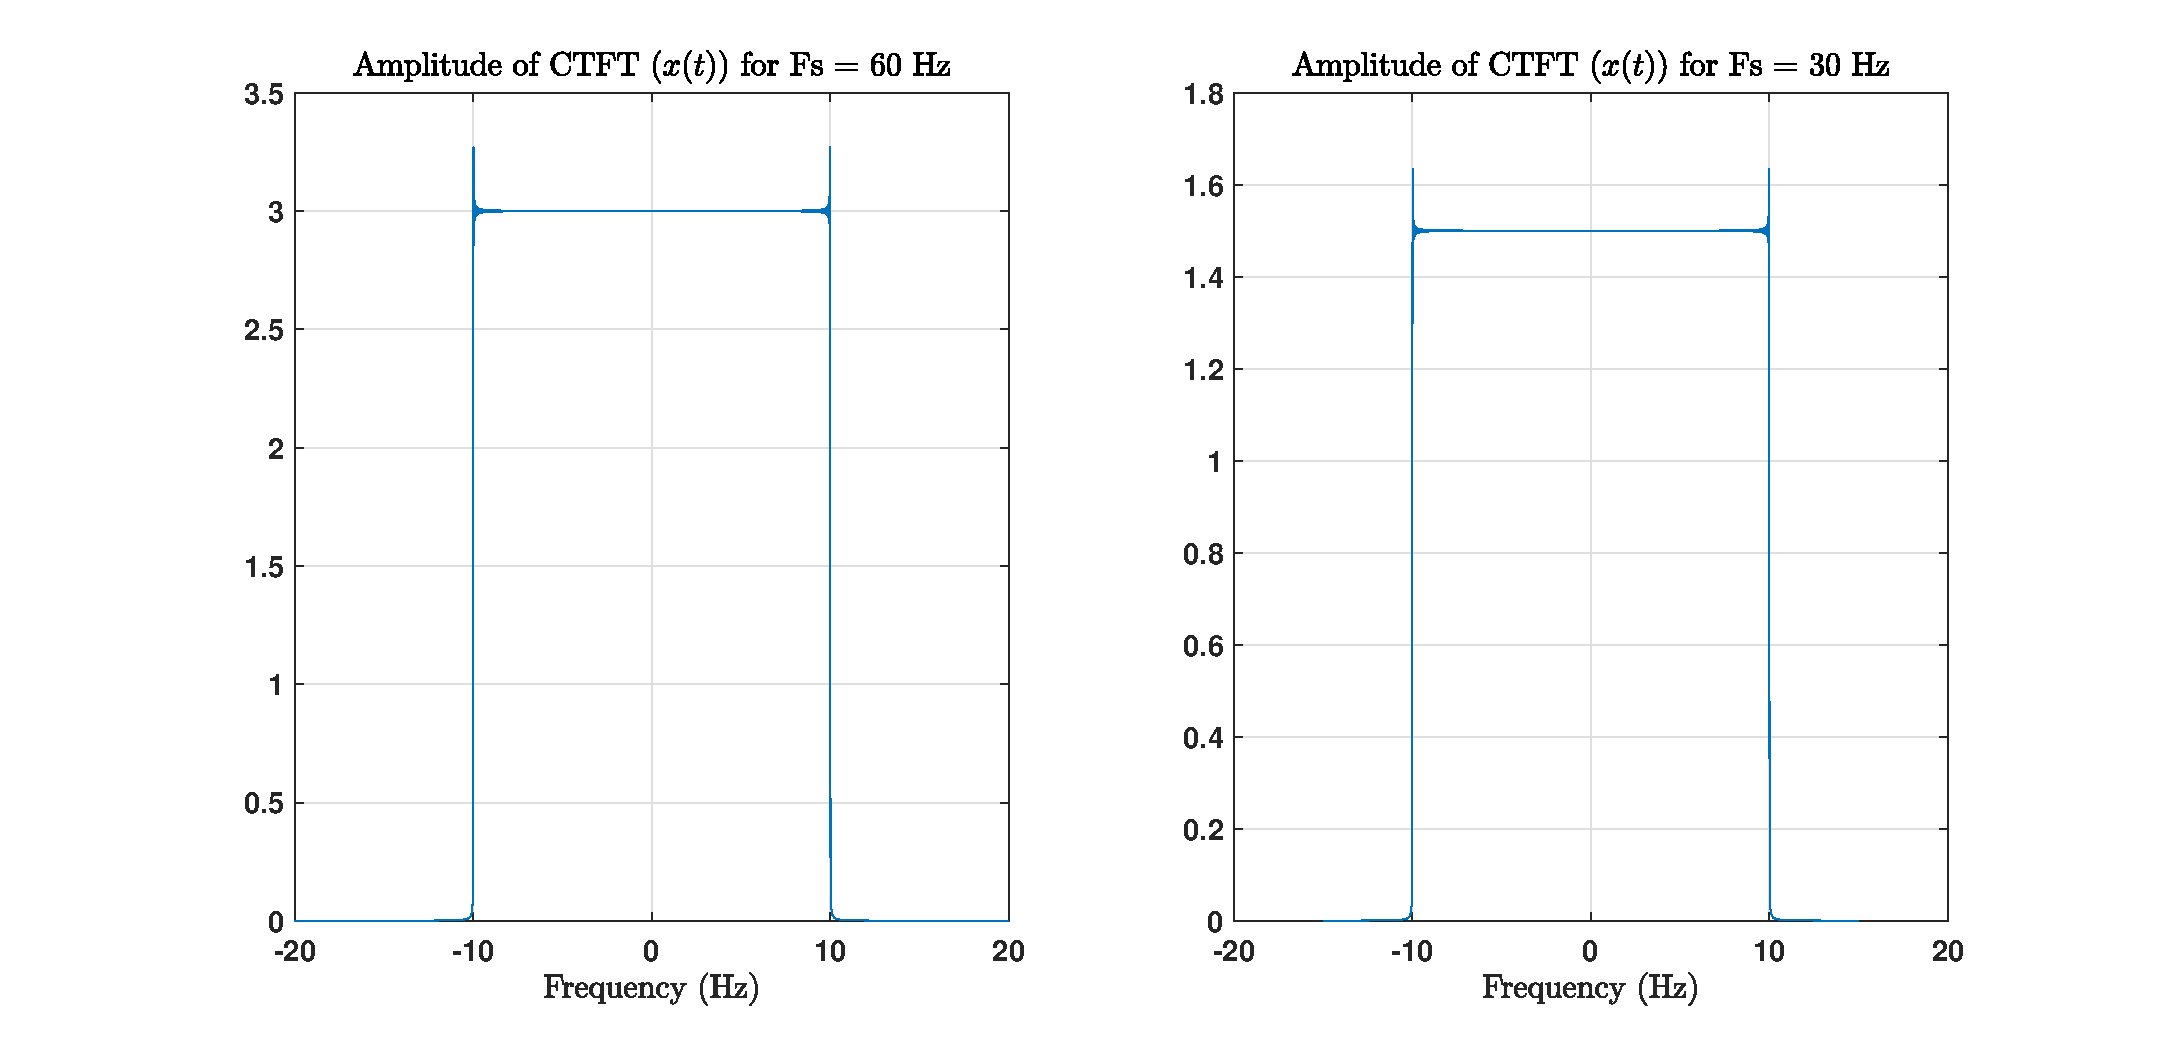
\includegraphics[scale = 0.4]{Figures/Sim_dowsampling_upsampling/CTFT_Amp_Sinc_B_10_Fs_30_60}
\caption{CTFT Amplitude Spectrum}
\label{fig:Sim_dowsampling_upsampling:CTFT_Amp_Sinc_B_10_Fs_30_60}
\end{figure}


\begin{figure}[ht]
\centering
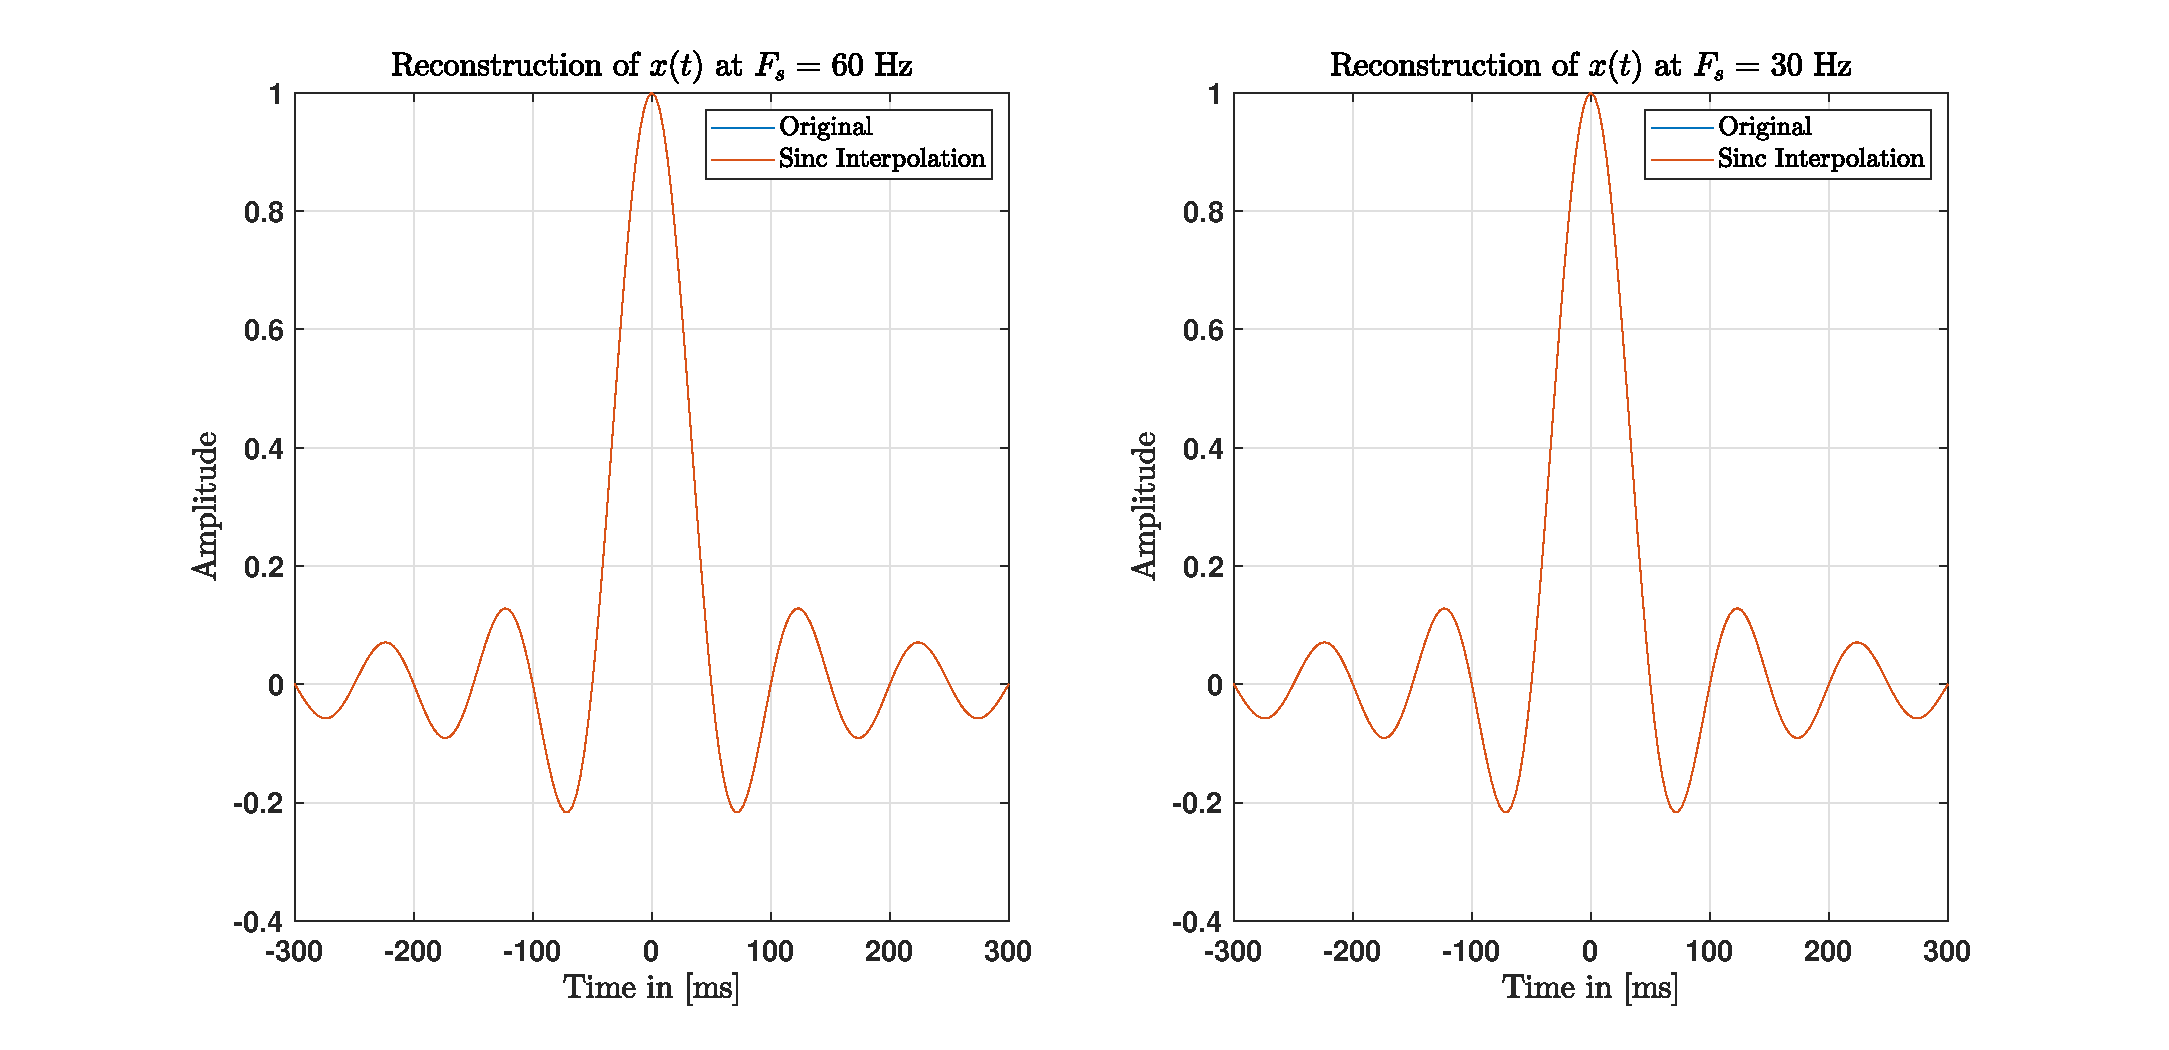
\includegraphics[scale = 0.4]{Figures/Sim_dowsampling_upsampling/Interpolation_Sinc_Fs_30_60_Hz_B_10_Hz}
\caption{Ideal Reconstruction}
\label{fig:Sim_dowsampling_upsampling:Interpolation_Sinc_Fs_30_60_Hz_B_10_Hz}
\end{figure}


\newpage

\item Now I decide to choose a $F_s \, < \, F_{\text{Nyquist}}$

\begin{itemize}
    \item From theory, when we drop $F_s$ below $F_{\text{Nyquist}} \,  \equiv \, \Omega_s \, < \, 2\, \Omega_H$, \textit{aliasing} should occur
\end{itemize}

\begin{figure}[ht]
\centering
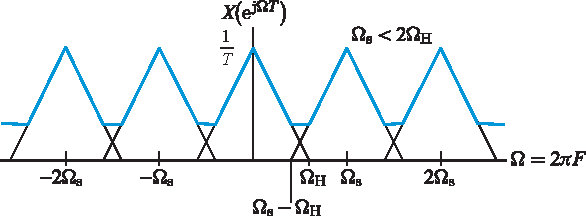
\includegraphics[scale = 0.9]{Figures/Sim_dowsampling_upsampling/aliasing_illustration}
\caption{Aliasing when $\Omega_s \, < \, 2\, \Omega_H$ \cite{DSP_DimitrisManolakis}}
\label{fig:Sim_dowsampling_upsampling:aliasing_illustration}
\end{figure}

\begin{itemize}
    
    \item From \autoref{fig:Sim_dowsampling_upsampling:aliasing_illustration}, we can say that:
    
    \begin{enumerate}
        \item Part of the spectrum is preserved and the other part which \textit{don't respect Nyquist theorem} is distorted
        
        \item But the signal spectrum still at $\Omega_H$ but distorted (I will clarify this point later in simulation)
    \end{enumerate}

    \item I tried to take $F_{s_{\text{ch}}} \, = \, 15$ Hz
    
    \item Result:
    
\end{itemize}

\begin{figure}[ht]
\centering
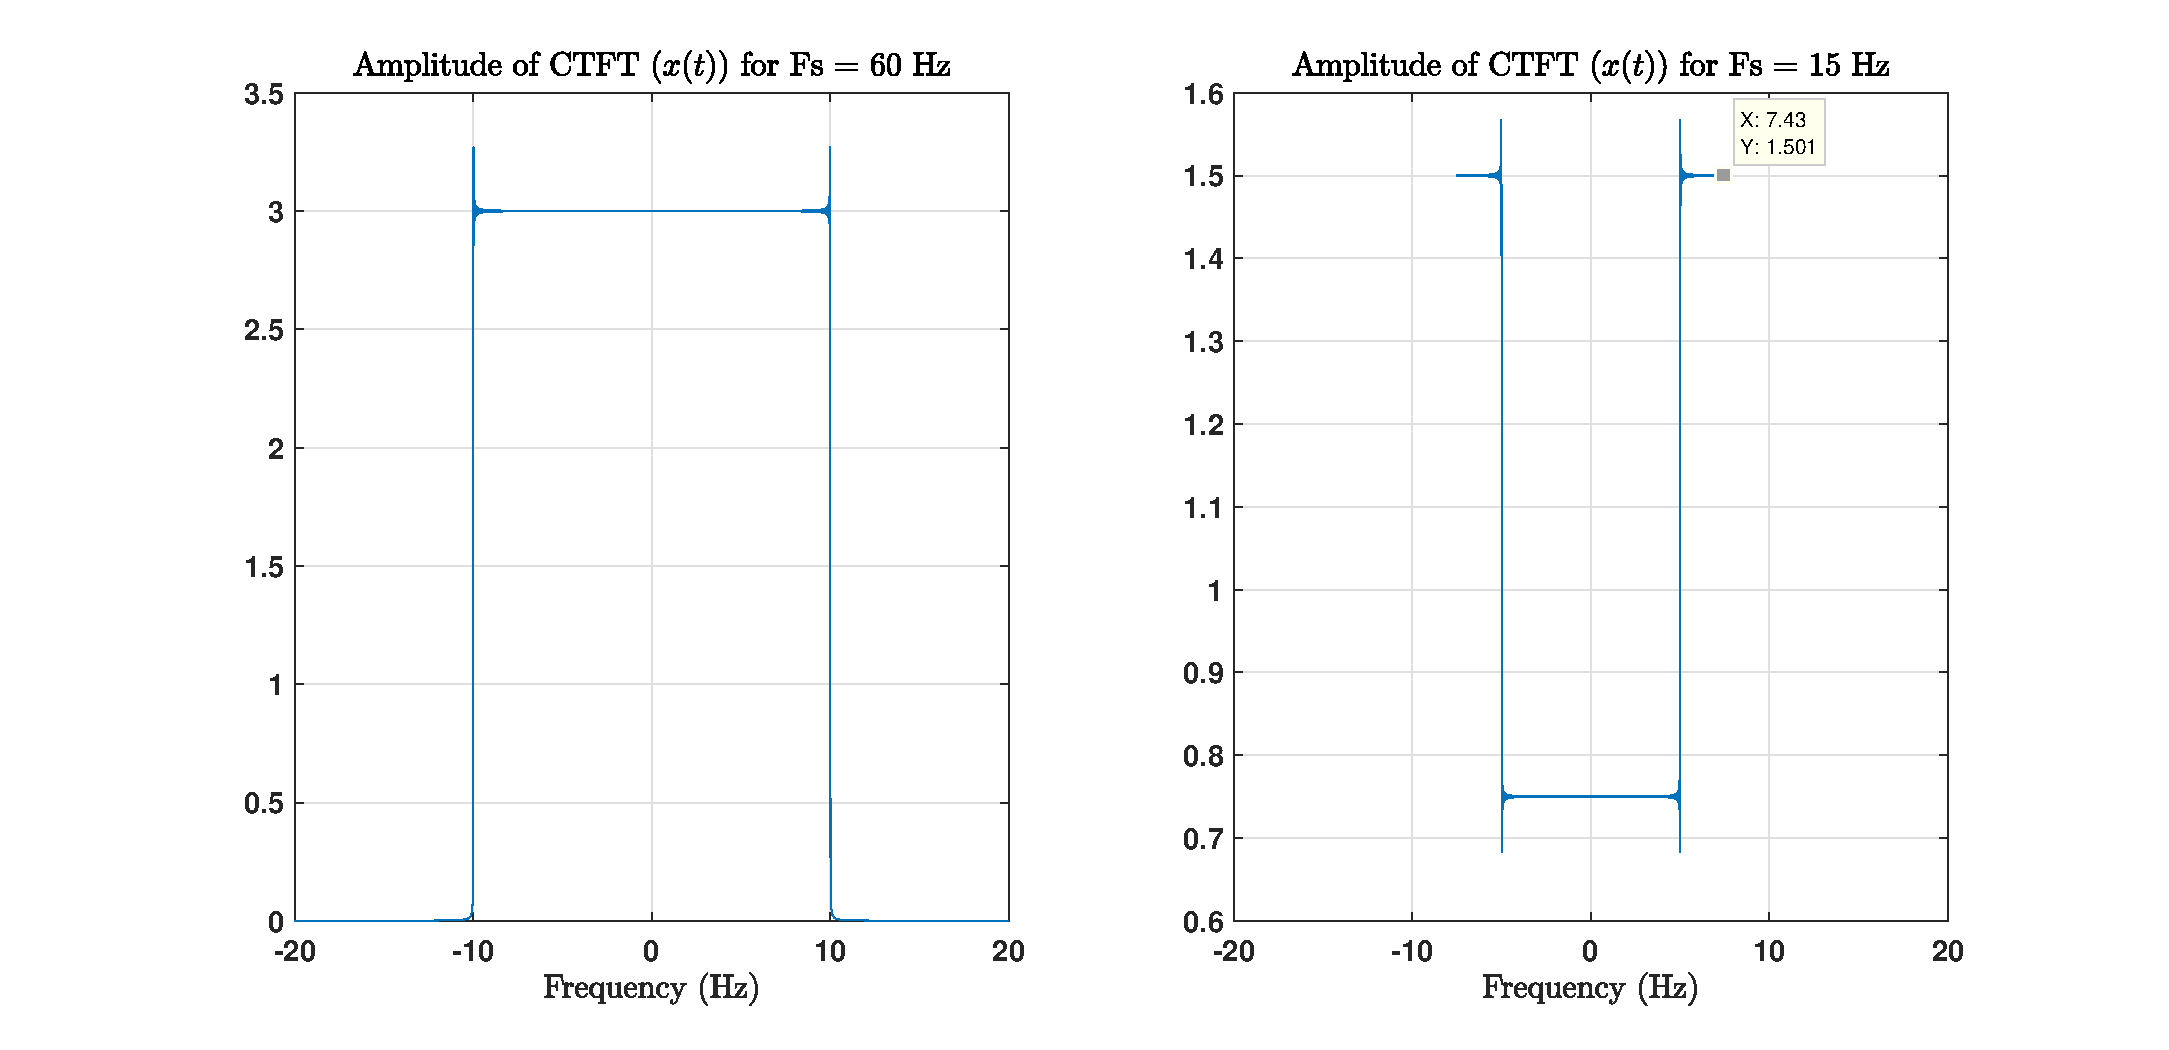
\includegraphics[scale = 0.45]{Figures/Sim_dowsampling_upsampling/CTFT_Amp_Sinc_B_10_Fs_60_15.eps}
\caption{Aliasing using $F_{s_{\text{ch}}} \, = \, 15$ Hz}
\label{fig:Sim_dowsampling_upsampling:CTFT_Amp_Sinc_B_10_Fs_60_15}
\end{figure}

\begin{itemize}
    \item the $F_s \, = \, 60$ Hz is just a reference, to compare aliased and unaliased spectrum
    
    \item For $F_s \, = \, 15$ Hz, my spectrum limit stop at 7.5 Hz and not at $B \, = \, 10$ Hz
    
    \begin{itemize}
    
        \item From my understanding of aliasing, I should get a spectrum of width $= \, B \, = \,10$ Hz, but distorted some how (addition of replica,from frequency exactly start the distortion,$\cdots$)
    
        \item This is because usually when simulating aliasing , I use fft(samples), where the samples are the downsampled giving a rate of 15 Hz (this is logic)
        
        \item \textit{But} (this is the important part) for frequency bins (which we as programmers generate): I generate it from $\displaystyle\frac{-F_s}{2} \, \rightarrow \, \displaystyle\frac{F_s}{2}$
        
        \item Doing so is fine when $F_s \,  > \, F_{\text{Nyquist}}$: In the left plot of \autoref{fig:Sim_dowsampling_upsampling:CTFT_Amp_Sinc_B_10_Fs_60_15} for $F_s \, = \, 60$ Hz, I did so and the spectrum is fine
        
        \item For the case of aliasing where $F_s \, = \, 15$ Hz, $\displaystyle\frac{-F_s}{2} \, \rightarrow \, \displaystyle\frac{F_s}{2} \, = \, -7.5 \, \rightarrow \, 7.5$ Hz
        
        
        \item However, I didn't in my life generate a frequency bins when taking an alias case, since in normal signal processing, we prevent aliasing and respect Nyquist sampling condition
        
        \item Clearly I need a more general way to implement aliasing in a correct way
        
    \end{itemize}
    
\end{itemize}

\newpage
\item I did some search, and I found this example from  matlab  documentation
    
    \begin{itemize}
        \item As motivation, when I search for examples to simulate aliasing over a full range of frequencies from $0 \, \rightarrow \, B$[Hz], it was the only convenient one
        
        \item Put the picture of the replicated spectrum when doing sampling, and say that my target is to simulate the idea that when sampling below Nyquist rate, distortion arise
        
        \item All other resources focus only on sin or cos (so only 1 active frequency component).\\
        
        \todo{aliasing resources} to cite the aliasing resource I have

    \end{itemize}
    
\item The example use discrete time approach, which is shown in \autoref{fig:Sim_dowsampling_upsampling:aliasing_demo_matlab_doc}
  
\begin{figure}[ht]
\centering
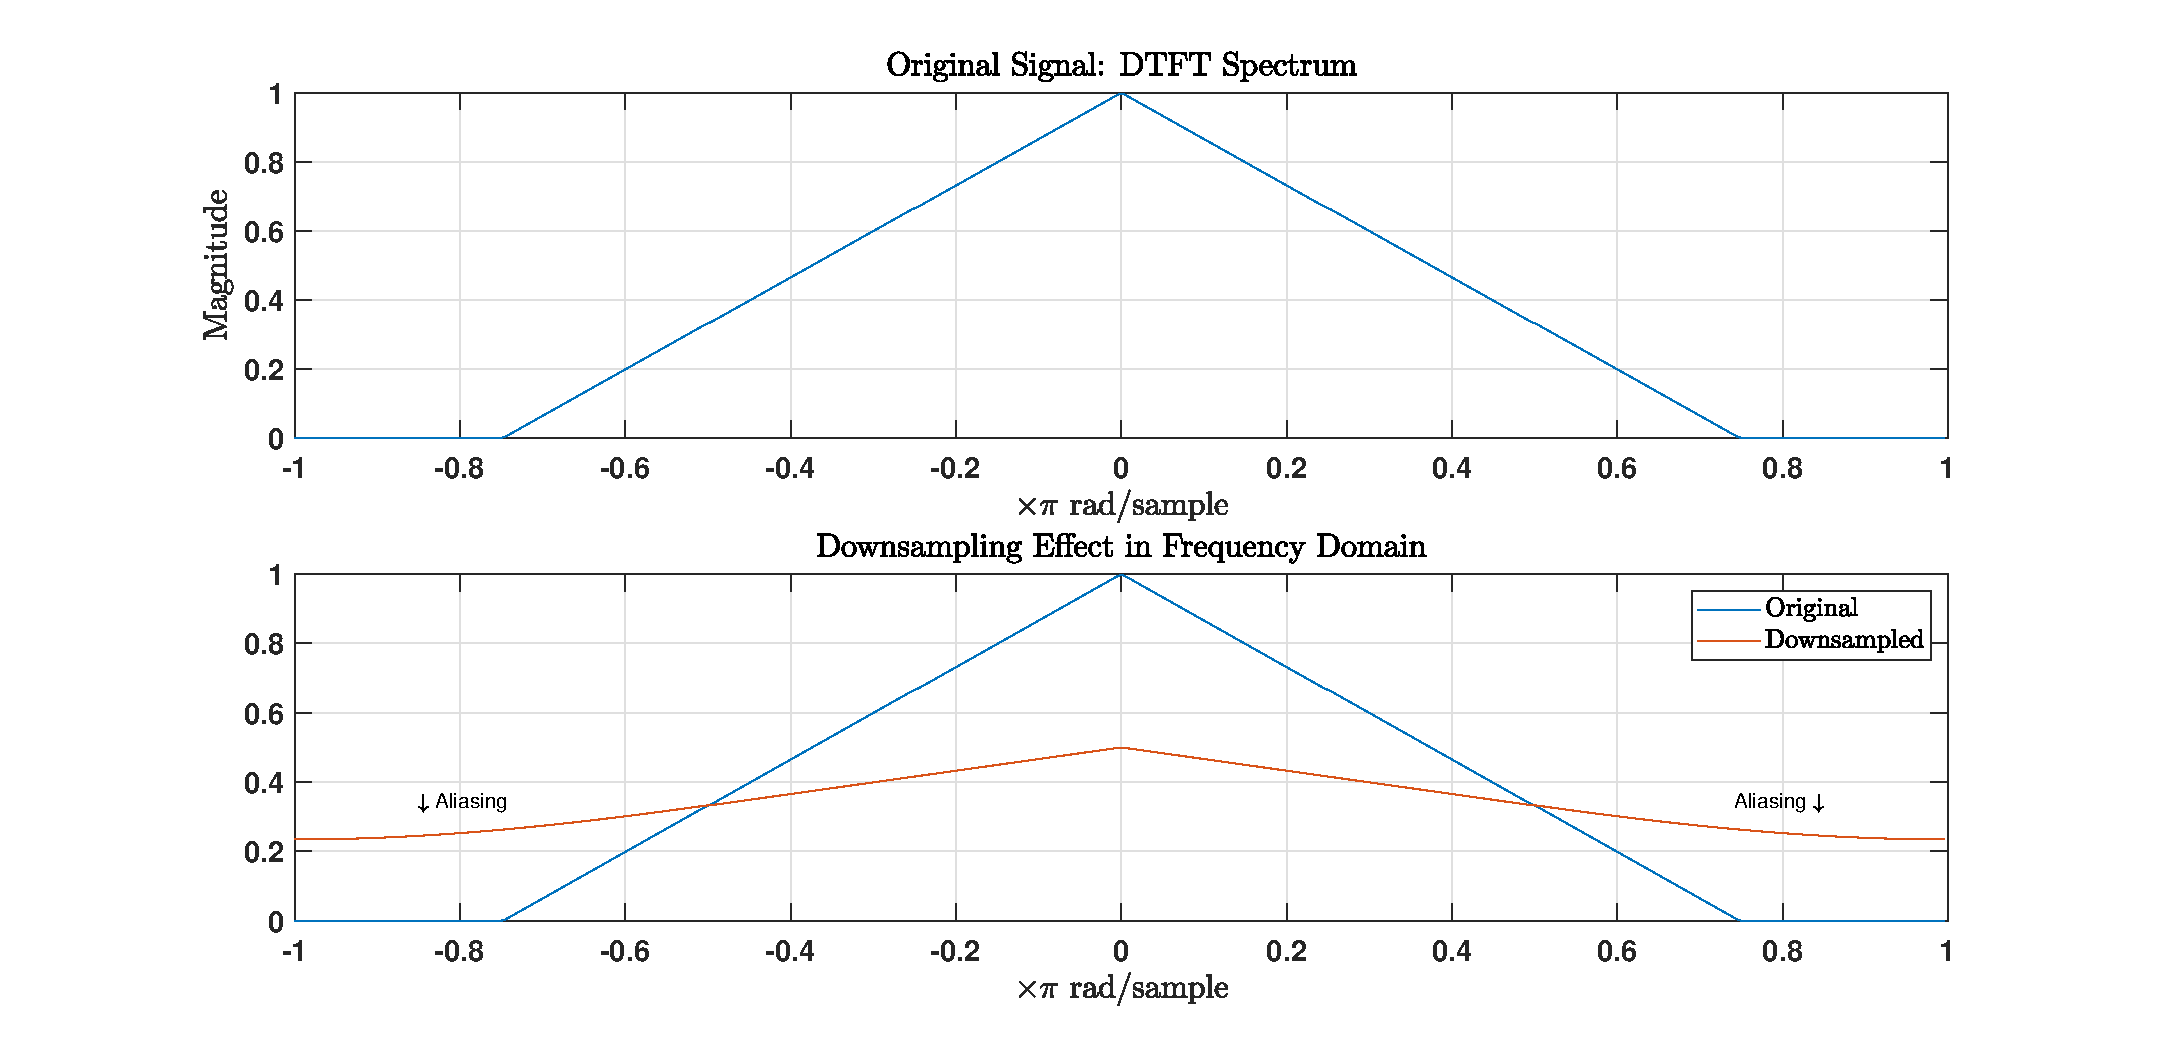
\includegraphics[scale = 0.45]{Figures/Sim_dowsampling_upsampling/aliasing_demo_matlab_doc}
\caption{Aliasing Example in discrete approach}
\label{fig:Sim_dowsampling_upsampling:aliasing_demo_matlab_doc}
\end{figure}  
    
\item \underline{Explanation of \autoref{fig:Sim_dowsampling_upsampling:aliasing_demo_matlab_doc}}    
    
    \begin{itemize}
    
    \item A \textit{discrete time bandlimited signal}   is generated, where the \textit{discrete bandwidth}  $= \, 0.75 \pi$ rad/cycle
    
    \item We do an integer downsampling operation of $D \, = \, 2$
    
    \item Recall that dowsampling doesn't necessary causes aliasing
    
    \item To know whether aliasing occurred or not, we test the following condition:
    
    \begin{equation}
    \text{Discrete Spectral support} \, < \, \displaystyle\frac{2 \pi}{D}
    \label{Eq:Aliasing_condition_discrete_freq_approach}
    \end{equation}
    
    \begin{itemize}
        \item If this is true, then dowsampling by $D \in \mathbb{N}$ won't cause aliasing
        
        \item If not, then aliasing occur
    \end{itemize}
    
    \item Back to the example, the \textit{Discrete Spectral support} contains \textit{positive discrete bandwidth} and the \textit{negative part} $\rightarrow$ \textit{Discrete Spectral support} $ \, = \, 0.75 \pi \, \times \, 2 \,  = \, 1.5 \, \pi$ rad/cycle
    
    \item Testing \autoref{Eq:Aliasing_condition_discrete_freq_approach} for $D \, = \, 2$, we get: $1.75 \pi > \displaystyle\frac{2 \pi}{D \, = \, 2} \, = \, \pi \rightarrow$ aliasing occur
    
    \begin{itemize}
        \item Spectral copies will overlap and get added
    \end{itemize}
    
    
    \item Although that aliasing is shown, \textit{but} there is no mention to any $F_s$ or ($T_s$): the example is simulated assuming that we are getting the discrete samples some how
    
    \begin{itemize}
        \item Recall that in our case (not just my case but also in real world), we express everything in Hz, seconds,$\cdots \leftrightarrow$ some meaningful units
        
        \item To get back from from radian/cycle $\rightarrow$  Hz, we use \cite{DSP_DimitrisManolakis}:
        
        \begin{equation}
                F \, [\text{Hz}] \, = \, \omega [\text{radian/cycle}] \, \times \, \left( \, \displaystyle\frac{F_s}{2 \pi} \, \, \right)
                \label{Eq:freq_conversion_rad_to_Hz}
        \end{equation}
        
        \item However, \autoref{Eq:freq_conversion_rad_to_Hz} is normally used when Nyquist theorem is respected $\leftrightarrow \, F_s \, > \, 2 \, \times f_{\text{max}}$
        
        \item But in our case, it is not
        
        \item So this give me a question, what $F_s$ should I use to obtain correctly a distorted spectrum according to \autoref{fig:Sim_dowsampling_upsampling:aliasing_illustration}
        
    \end{itemize}
    
        \item Put frequency conversion formula
        
        \item All the overlapping and the spectrum is inside $[-\pi \, , \, \pi]$, even when aliasing occurs
        
        \item Show the plot of a aliased sinc now, and compare it to the left plot of \autoref{fig:Sim_dowsampling_upsampling:CTFT_Amp_Sinc_B_10_Fs_60_15} 
        
    \end{itemize}

\item Applying concept in the example of \autoref{fig:Sim_dowsampling_upsampling:aliasing_demo_matlab_doc} to my case of sinc signal, where $B \, = \, 10$ Hz and $F_{s_{\text{ch}}} \, = \, 15$ Hz: 
        
\item Now when finishing from simulating in the discrete frequency domain, we need to move to the continuous frequency domain (that is $F$[Hz])

\begin{itemize}
    \item However, I have a problem which $F_s$ to use
     when doing the conversion
    
    
\end{itemize}


    
\end{itemize}



%*****************************************************
%*****************************************************
%*****************************************************


\chapter{Random Process}

In this chapter, we see how to generate white noise with correct PSD.\\


Assuming a baseband model of bandwidth $B$ Hz, and AWGN channel, the total noise power is the area

\begin{figure}[ht]
\centering
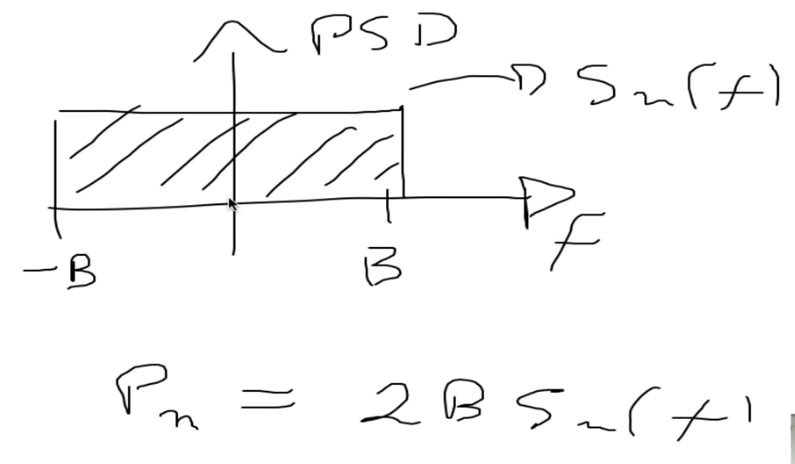
\includegraphics[scale = 0.5]{Figures/Random_Process/Total_Noise_Power_AWGN}
\caption{PSD for AWGN Baseband Model}
\label{fig:Random_Process_Total_Noise_Power_AWGN}
\end{figure}

From random process, the power of random sequence $X[n]$ is equal to the mean square, that is $E[X^2]$.

Now if this sequence have zero mean, then the mean square will be equal to the variance $\leftrightarrow \, E[X^2] \, = \, \sigma$.

So if want to generate some  noisy sequence having some total power (whih is equal to $\sigma$), we simply multiply the noisy sequence generated with the standard deviation $\sqrt{\sigma} \leftrightarrow \, $ 


%*****************************************************
%*****************************************************
%*****************************************************




\printglossary[type=\acronymtype]


%******************** References *********************

\bibliographystyle{IEEEtran}

\bibliography{Literature/Books_Signal_Processing,Literature/Communication_Systems,Literature/Papers_Signal_Processing,Literature/Papers_Sampling}


%*************************************************
%*************************************************


\end{document}